% !TEX root = ./manuscript.tex
%  LaTeX support: latex@mdpi.com
%  In case you need support, please contact latex@mdpi.com
%=================================================================
\documentclass[agriengineering,article,submit,pdftex,moreauthors]{Definitions/mdpi}

% Additional packages
\usepackage{siunitx}
\usepackage{booktabs}
\usepackage{pdflscape}
\usepackage{multirow}
\usepackage{float}
\usepackage{placeins}
\usepackage{tikz}
\usetikzlibrary{positioning, arrows.meta, fit, backgrounds, calc}
\usepackage{xr-hyper}
\externaldocument{supplementary}

% Let the MDPI class load hyperref with its default bluecite link colour
% so internal cross-references and citations are visibly clickable.

%=================================================================
% MDPI internal commands - do not modify
\firstpage{1}
\makeatletter
\setcounter{page}{\@firstpage}
\makeatother
\pubvolume{1}
\issuenum{1}
\articlenumber{0}
\pubyear{2026}
\copyrightyear{2026}
\datereceived{ }
\daterevised{ }
\dateaccepted{ }
\datepublished{ }
\hreflink{https://doi.org/}

%=================================================================
% Paths for figures
\graphicspath{
  {figures_final/}
}

%=================================================================
% Title
\Title{Winter-Chill Attribution and CMIP6 Projections of ENSO-Driven Olive Yield Collapse on the Hyper-Arid Peruvian Coast}

\TitleCitation{Winter-Chill Attribution and CMIP6 Projections of Olive Yield Collapse on the Peruvian Coast}

% Author ORCID IDs
\newcommand{\orcidauthorA}{0000-0002-5283-7211} % J. Quille-Mamani
\newcommand{\orcidauthorB}{0009-0003-8511-4524} % J. Huanuqueño-Murillo
\newcommand{\orcidauthorC}{0000-0003-3325-5512} % D. Quispe-Tito
\newcommand{\orcidauthorD}{0000-0002-4518-1023} % G. Huayna-Felipe
\newcommand{\orcidauthorE}{0000-0003-2236-8335} % J. Espinoza-Molina
\newcommand{\orcidauthorF}{0000-0003-1872-9062} % K. Acosta-Caipa
\newcommand{\orcidauthorG}{0009-0003-8329-6555} % H. S. Pérez-Cubas
\newcommand{\orcidauthorH}{0000-0002-0421-399X} % E. Ingol-Blanco
\newcommand{\orcidauthorI}{0000-0003-3946-7188} % L. Ramos-Fernández
\newcommand{\orcidauthorJ}{0000-0001-7432-4364} % E. Pino-Vargas

% Authors
\Author{Javier Quille-Mamani $^{1}$\orcidA{},
Jos\'{e} Huanuque\~{n}o-Murillo $^{2}$\orcidB{},
David Quispe-Tito $^{2}$\orcidC{},
German Huayna-Felipe $^{3}$\orcidD{},
Jorge Espinoza-Molina $^{4}$\orcidE{},
Karina Acosta-Caipa $^{4}$\orcidF{},
Heler Samir P\'{e}rez-Cubas $^{5}$\orcidG{},
Eusebio Ingol-Blanco $^{6}$\orcidH{},
Lia Ramos-Fern\'{a}ndez $^{2,}$*\orcidI{} and
Edwin Pino-Vargas $^{7,}$*\orcidJ{}}

\AuthorNames{Javier Quille-Mamani, Jos\'{e} Huanuque\~{n}o-Murillo, David Quispe-Tito, German Huayna-Felipe, Jorge Espinoza-Molina, Karina Acosta-Caipa, Heler Samir P\'{e}rez-Cubas, Eusebio Ingol-Blanco, Lia Ramos-Fern\'{a}ndez, Edwin Pino-Vargas}
\AuthorCitation{Quille-Mamani, J.; Huanuque\~{n}o-Murillo, J.; Quispe-Tito, D.; Huayna-Felipe, G.; Espinoza-Molina, J.; Acosta-Caipa, K.; P\'{e}rez-Cubas, H.S.; Ingol-Blanco, E.; Ramos-Fern\'{a}ndez, L.; Pino-Vargas, E.}

\address{%
$^{1}$ \quad Geo-Environmental Cartography and Remote Sensing Group (CGAT), Universitat Polit\`{e}cnica de Val\`{e}ncia, Cam\'{i} de Vera s/n, 46022 Valencia, Spain\\
$^{2}$ \quad Department of Water Resources, National Agrarian University La Molina, Lima 15024, Peru\\
$^{3}$ \quad Master's Program in Water Resources, Jorge Basadre Grohmann National University, Tacna 23000, Peru\\
$^{4}$ \quad Department of Architecture, Jorge Basadre Grohmann National University, Tacna 23000, Peru\\
$^{5}$ \quad Department of Hydraulic Engineering and Environment, Universitat Polit\`{e}cnica de Val\`{e}ncia, Cam\'{i} de Vera s/n, 46022 Valencia, Spain\\
$^{6}$ \quad Department of Civil Engineering, New Mexico State University, Las Cruces, NM 88003, USA\\
$^{7}$ \quad Department of Civil Engineering, Jorge Basadre Grohmann National University, Tacna 23000, Peru}

\corres{Correspondence: liarf@lamolina.edu.pe (L.R.-F.); epinov@unjbg.edu.pe (E.P.-V.)}

%=================================================================
% Abstract
\abstract{Olive (\textit{Olea europaea} L.) orchards on the hyper-arid Peruvian coast (Tacna, $18^{\circ}$~S) suffered $>70\,\%$ yield collapses in the 2016 and 2024 El~Ni\~{n}o seasons against a non-failure mean of ${\sim}6$~t~ha$^{-1}$ and a 2022 La~Ni\~{n}a bumper harvest, raising the question of whether insufficient winter chilling is the binding climate constraint. We combined in-situ daily meteorology (2015--2025) with yield records from eleven Sevillana--Ascolana parcels (88 parcel-years over eight seasons) and fitted a year-level log-OLS model with mean chill-window and fruit-growth temperatures, validated by year-block bootstrap, permutation, a closed-form Bayesian posterior and a parcel-year mixed model. The model achieves $R^{2}_{\log}=0.65$, and the chill slope ($\beta=-0.82$) is robust across three independent tests: one-sided permutation $p=0.036$; Bayesian posterior with 99.8\,\% of mass below zero (Savage--Dickey BF$_{10}=15.9$); parcel-year mixed model $p<10^{-14}$. Counterfactual restoration of chill-window temperature to its non-failure climatology recovers the full collapse in both years, whereas restoring fruit-growth temperature recovers nothing. CMIP6 delta-method projections identify a chill-collapse threshold at $\Delta T_{\text{winter}}\approx +1.25\,^{\circ}$C; SSP1-2.6 alone reduces mid-century mean yield by ${\sim}52\,\%$, and SSP5-8.5 reaches $-89\,\%$ by 2051--2070. Tacna emerges as a chill-sentinel system where winter warmth, not summer heat, is the binding constraint and the transition to the failure regime lies on a near-term adaptation horizon.}

\keyword{\textit{Olea europaea}; winter chill attribution; mean chill-window temperature; counterfactual decomposition; CMIP6 delta method; ENSO; Humboldt Current; Tacna}

\externalbibliography{yes}

%=================================================================
\begin{document}

%=================================================================
\section{Introduction}
\label{sec:introduction}

Climate change is altering the suitability of perennial fruit and tree crops worldwide~\cite{ipcc2023climate,ortizbobea2021,benmoussa2017,parker2019}. For deciduous and evergreen species with a chilling requirement, the most direct mechanism is the failure of winter chill accumulation: warm winters reduce the dormancy-completion signal that prepares the buds for synchronous spring bud-break, flowering, and fruit set, with downstream effects on yield, fruit quality, and inter-annual stability~\cite{luedeling2012,aguilera2014,darbyshire2016,parker2019}. Olive (\textit{Olea europaea} L.) is a textbook example: although it is often labelled as Mediterranean and drought-tolerant, its inflorescence-induction physiology is chill-driven, and trials in warm subtropical climates have repeatedly shown that insufficient winter chilling produces poor flowering, irregular bearing, and outright crop failure~\cite{deMeloAbreu2004,rallo2013,fernandez2023chill}.

Despite this physiological consensus, the quantitative attribution of \emph{specific} yield-collapse events to chill-window warming remains rare in the olive literature. Most studies either (i)~work in regions where the chill regime is comfortably above the dormancy-completion threshold, so that observed inter-annual variability is dominated by water and pruning management, or (ii)~project future risk under climate scenarios without anchoring the projection in a documented historical failure event~\cite{aguilera2014,fraga2020,mairech2021,fernandez2023chill,grillakis2022olive,picornell2023olive}. The southern Peruvian Pacific coast (${\sim}18\,^\circ$S) occupies an unusual position in this landscape: the cold Humboldt current keeps daily summer $T_{\max}$ below the canonical $35\,^\circ$C heat-stress threshold for olive across the entire record (KDD$_{35}=0$), yet leaves winter $T_{\text{mean}}$ only marginally below the chill-collapse temperature. Under this configuration, even modest interannual warming --- for example during canonical El~Ni\~{n}o--Southern Oscillation (ENSO) warm-phase events --- can flip the system from a productive into a failure regime. The inter-annual yield range on the same eleven mature Sevillana--Ascolana parcels spans from $12.06$~t~ha$^{-1}$ in 2022 (a triple La~Ni\~{n}a winter) to $0.68$~t~ha$^{-1}$ in 2024 (post-El~Ni\~{n}o 2023/24) --- an 18-fold swing within three harvest campaigns. This contrast is substantially larger than the typical alternate-bearing oscillations reported for olive~\cite{lavee2007alternate} and ranks among the sharpest documented climatic-forcing signals in the Peruvian olive belt~\cite{pinovargas2022enso,chucuya2022}, offering an unusually clean anchor for a chill-attribution exercise rather than a low-signal correlational gradient.

Three properties make this system a uniquely tractable natural experiment for chill attribution. First, the eleven parcels are managerially homogeneous (same Sevillana--Ascolana cultivar pair, same age class, same irrigation regime, same farm) so that inter-annual variability is dominated by climate rather than by management. Second, two failure seasons (2016 and 2024) and one extreme bumper season (2022) coincide with two of the strongest El~Ni\~{n}o events of the satellite era and the first triple-dip La~Ni\~{n}a in half a century, providing the cleanest possible climatic forcing contrast. Third, the southern Peruvian coast at $18\,^\circ$S has continuous \emph{in-situ} daily meteorology and excellent Sentinel-2 coverage during the reproductive window (October--February)~\cite{drusch2012,wu2023rs}, making it possible to reconstruct the entire chill-to-yield causal chain at the parcel level.

Beyond historical attribution, quantifying how this chill margin will evolve under future climate requires a projection framework. The delta method~\cite{luedeling2012,hannah2013} --- adding seasonal warming increments from the Coupled Model Intercomparison Project Phase~6 (CMIP6) to an observed baseline --- remains the standard approach for chill projections when raw GCM output is known to be biased at coastal grid cells, as is the case along the Humboldt-cooled South American Pacific~\cite{thrasher2022}. Prior CMIP6 chill-projection studies in olive have reported Chill-Portion reductions of 12--71\,\% by end-of-century in Crete~\cite{grillakis2022olive}, increased interannual flowering variability in the western Mediterranean~\cite{picornell2023olive}, and analogous warm-winter signatures in almond and other chilling-requiring species~\cite{benmoussa2017,fernandez2021warmwinters,jagermeyr2021}. However, these projection studies face a validation gap: without an observed collapse to cross-check against, the projected losses remain unanchored. Combining attribution and projection within a single calibrated response surface --- the approach we take here --- closes that gap.

In this study we therefore (i)~quantify the dependence of olive yield on winter-chill exposure and fruit-growth temperature using a year-level statistical model; (ii)~test by counterfactual restoration whether the 2016 and 2024 collapses are, within the calibrated response surface, more consistent with chill-window warming than with fruit-growth heat stress; (iii)~assess whether Sentinel-2 vegetation indices composited over the previous reproductive window add information beyond the climatic signal; and (iv)~project how the chill--yield relationship evolves under CMIP6 Shared Socioeconomic Pathway (SSP) scenarios using a delta-method propagation of the observed climate.

The contributions are: (1)~the first quantitative chill-window attribution of olive yield collapse for the Peruvian olive belt; (2)~a methodologically novel chill--yield model formulation in which the headline predictor is the \emph{mean chill-window temperature} rather than the threshold-based Chill Portions count, an approach that is more robust at the warm tail of the chill-collapse curve where CP saturates at zero; (3)~an event-based counterfactual decomposition that isolates the chill channel from the co-varying heat channel using an \emph{in-situ} non-failure climatology as the reference state --- an identification strategy that sidesteps the coastal-grid bias affecting GCM-with/without-forcing counterfactuals along the Humboldt margin; (4)~a CMIP6 delta-method projection in which the mechanistic chill-collapse threshold ($\Delta T_{\text{winter}}\approx +1.25\,^\circ$C) is identified directly from the calibrated response surface; and (5)~a multi-layer robustness framework --- year-block bootstrap, permutation testing, parcel-random-intercept mixed-effects, Bayesian shrinkage prior, and dedicated VPD and alternate-bearing sensitivity checks --- that defends the attribution against the $n{=}8$ small-sample and confounding concerns.

%=================================================================
\section{Materials and Methods}
\label{sec:materials_methods}

\subsection{Study Area}
\label{sec:study_area}

The study is located at a single commercial olive orchard in the La Yarada--Los Palos district of the Caplina basin, Tacna, southern Peru (orchard centroid $18^\circ10'55''$~S, $70^\circ31'52''$~W; Figure~\ref{fig:study_area}). The climate is a warm-coastal hyper-arid desert (Köppen BWh) cooled year-round by the Humboldt upwelling current; mean annual precipitation is below 30~mm and irrigation is by surface canal complemented by groundwater pumping from the La Yarada aquifer~\cite{chucuya2022,pinovargas2022enso}. The eleven parcels (mean area $1.25$~ha; total $\approx 13.7$~ha) are uniformly planted with the Sevillana--Ascolana cultivar pair on rootstocks of the same age class (planted $\approx 2004$; 22~years old at the time of analysis, fully mature throughout the study period).

\begin{figure}[H]
\centering
\includegraphics[width=\textwidth]{Figure1.png}
\caption{Study area. (\textbf{a})~Location of Peru in South America. (\textbf{b})~Location of the Tacna region (red box) within southern Peru. (\textbf{c})~Olive orchard boundary ($\approx 13.7$~ha) in the La Yarada--Los Palos district of the Caplina basin at $18^\circ10'55''$~S, $70^\circ31'52''$~W, showing the eleven Sevillana--Ascolana parcels analysed in this study and the co-located automatic weather station (AWS).\label{fig:study_area}}
\end{figure}

The two cultivars are interplanted in alternating rows at a $7\times 7$~m spacing within each parcel, with Ascolana acting as the principal pollinator for the dominant Sevillana cultivar; this arrangement is uniform across all eleven parcels, so the cultivar mix does not vary as a between-parcel factor. Both cultivars share the same canopy architecture (open vase, mean canopy height $\approx 4$~m), the same chilling requirement class~\cite{deMeloAbreu2004,rallo2013}, and a synchronous flowering and fruit-maturation phenology, so the parcel block is treated as a single spectral and phenological unit.

All parcels share the same irrigation schedule and fertilisation programme; pest and disease pressure was reported as low and uniform across parcels by the orchard management throughout the study period (no phytosanitary treatments were applied differentially among parcels). According to the orchard's operational records, the irrigation regime, pruning protocol and fertilisation schedule were also stable \emph{between years} across the 2015--2025 period, with the sole exception of the 2021 campaign (see Section~\ref{sec:yield_records}). The forced 2021 rest may have primed an unusually strong on-year rebound in 2022, which we flag explicitly rather than absorb into the climate signal.

\subsection{Yield Records}
\label{sec:yield_records}

Annual olive yield was recorded at the parcel scale ($n=11$ parcels) for the 2016--2024 agricultural campaigns and is reported in tonnes per hectare (t~ha$^{-1}$). Yields were measured operationally by the orchard manager using calibrated field scales mounted on the harvest trailers and aggregated per parcel at the end of each campaign. The 2021 harvest was not collected because the orchard was idled by the COVID-19 pandemic; we treat 2021 as a structural exclusion (not a missing value to be imputed) and we deliberately retain both 2016 and 2024 in the analysis because they are the central attribution events of the paper. The eight calibration years that enter the year-level analysis are summarised, together with the climatic predictors defined in Sections~\ref{sec:meteo}--\ref{sec:heat_stress}, in Table~\ref{tab:year_level}; a detailed annual summary including yield standard deviations, additional phenology-window aggregates and ET$_0$ is given in Supplementary Table~\ref{tab:annual_summary}.

\subsection{Meteorological Data}
\label{sec:meteo}

Daily $T_{\min}$ and $T_{\max}$ were obtained from the AWS co-located with the orchard (Davis Vantage Pro2 Plus, Davis Instruments, Hayward, CA, USA; temperature accuracy $\pm 0.5\,^\circ$C; 15-minute logging interval) for 1~January~2015 to 2~December~2025 ($n=3388$ valid days after quality control). Quality control consisted of (i)~range checking against the regional climatology, (ii)~flagging of inverted $T_{\min}$/$T_{\max}$ pairs, and (iii)~gap-filling of fewer than three consecutive missing days by linear interpolation in temperature anomaly space. ENSO context was obtained from the NOAA Physical Sciences Laboratory Oceanic Ni\~{n}o Index (ONI) monthly time series.

Figure~\ref{fig:meteo} summarises the resulting record. Panel~(a) shows the daily $T_{\min}$--$T_{\max}$ range (grey band) and the 30-day centred rolling $T_{\text{mean}}$ (blue line); the May--August chill window of each calendar year is shaded and coloured red for El~Ni\~{n}o seasons (2015, 2023), blue for the La~Ni\~{n}a sequence 2020--2022 and grey for neutral seasons. The dashed horizontal line at $\approx 18\,^\circ$C is a visual reference for the chill-collapse regime identified in the continuous warming sweep of Section~\ref{sec:results_cmip6} (Figure~\ref{fig:warming_sweep}), corresponding to $\Delta T_{\text{winter}}\approx +1.25\,^\circ$C above the non-failure climatology of $\approx 16.7\,^\circ$C. Panel~(b) reports the chill-window mean temperature $T_{\text{chill},t-1}$ by chill year, computed from the hourly sinusoidal reconstruction of $T_{\min}$ and $T_{\max}$ following the \textit{chillR} convention~\cite{luedeling2018chillR,linvill1990chillhours}; bar colours follow the ENSO convention of panel~(a), and the $Y-1$ chill year and the corresponding harvest year $Y$ are given below each bar. The two El~Ni\~{n}o chill windows (2015 and 2023) stand out at $18.20\,^\circ$C and $18.45\,^\circ$C respectively, $\approx 1.5\,^\circ$C above the non-failure climatology; these are the two warm anchors that drive the 2016 and 2024 yield collapses analysed in Section~\ref{sec:results}.

\begin{figure}[H]
\centering
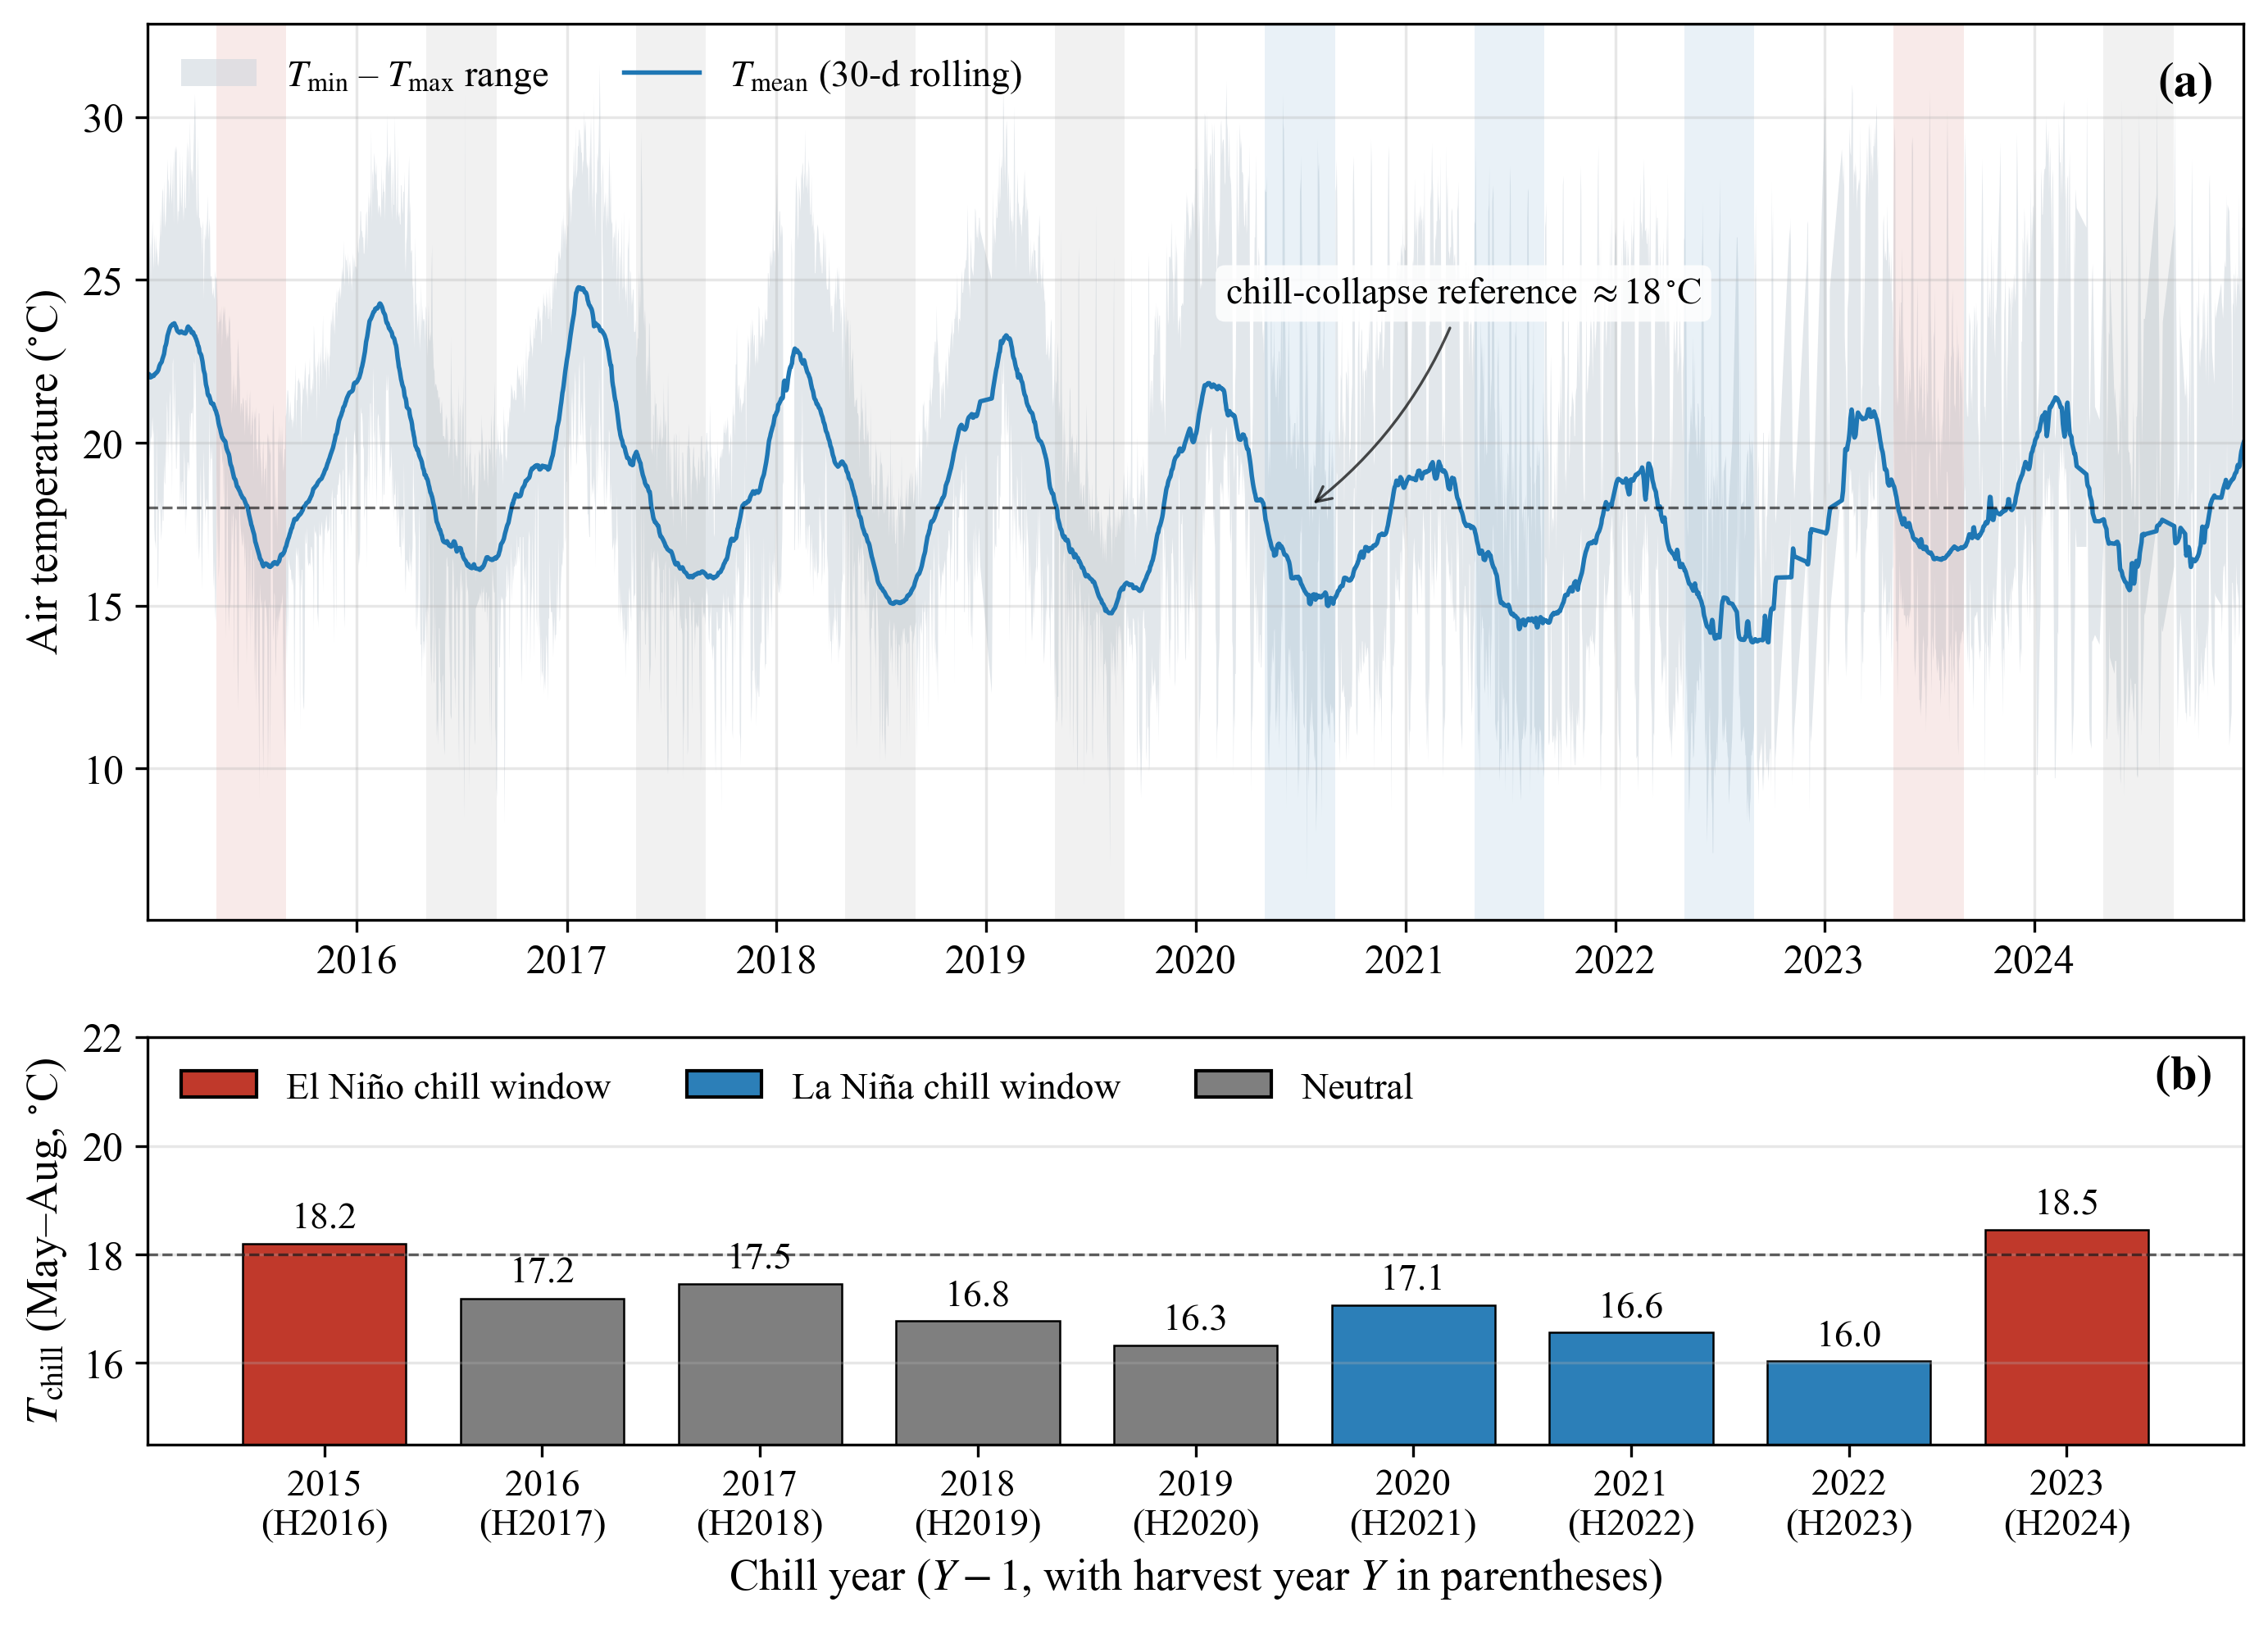
\includegraphics[width=\textwidth]{Figure2.png}
\caption{AWS meteorological overview for the orchard site, 2015--2024. (\textbf{a})~Daily $T_{\min}$/$T_{\max}$ range and 30-day rolling $T_{\text{mean}}$, with the May--August chill window of each year shaded by ENSO phase. (\textbf{b})~Chill-window mean temperature $T_{\text{chill},t-1}$ by chill year, with the corresponding harvest year $Y$ in parentheses below each bar. See main text for the full description of colour coding and reference lines.\label{fig:meteo}}
\end{figure}

\subsection{Chill Accumulation}
\label{sec:chill_models}

Daily $T_{\min}$ and $T_{\max}$ were disaggregated to hourly temperatures using a two-piece sinusoidal interpolation~\cite{linvill1990chillhours,deMeloAbreu2004}: $T_{\min}$ is placed at 06:00 local time and $T_{\max}$ at 14:00, with a rising half-sine over the 8-hour interval $06:00\to 14:00$ and a falling half-sine over the 16-hour interval $14:00\to 06:00$ of the following day. This is the standard scheme used in the \textit{chillR} R package~\cite{luedeling2018chillR,luedeling2021phenoflex} and in olive chill studies in subtropical settings~\cite{aguilera2014}.

Three chill-accumulation models were computed for cross-validation (Supplementary Figure~\ref{fig:S1}): (i)~the \textbf{Dynamic Model} of Fishman et al.~\cite{fishman1987a,fishman1987b} --- Chill Portions (CP), our primary metric, implemented after Luedeling~\cite{luedeling2018chillR,luedeling2021phenoflex}; (ii)~the \textbf{Utah Model}~\cite{richardson1974} --- Chill Units (CU); and (iii)~\textbf{Chill Hours} below 7.2$\,^\circ$C and 12.0$\,^\circ$C. Chill accumulation was integrated over the Southern Hemisphere chill window of 1~May to 31~August. Because olive budburst in this site occurs in austral spring (late August--early September) and flowering in October--November~\cite{machaca2022olive,larico2019olive}, the chill accumulation that determines the yield harvested in calendar year~$Y$ is the chill of $Y-1$; we therefore define $\text{chill\_year}=Y-1$ throughout. The phenology windows used for the climate aggregates are listed in Supplementary Table~\ref{tab:pheno_windows}.

In addition to the threshold-based chill counts we computed the \textbf{mean hourly air temperature over the May--August window}, $T_{\text{chill},t-1}$. As shown in Section~\ref{sec:results_corr}, this metric is a much stronger predictor of olive yield than CP itself in the warm-coastal Peruvian context, because in years with very warm winters CP collapses to exactly zero and loses all resolving power, whereas $T_{\text{chill},t-1}$ remains a continuous diagnostic of how \emph{deep} into the failure regime the chill window has fallen.

\subsection{Heat Stress and Phenology-Window Aggregates}
\label{sec:heat_stress}

We computed standard heat-stress indices (KDD$_{35}$, CDD$_{30}$, tropical nights, hot days $>32\,^\circ$C, Heat Index, GDD$_{10}$, Penman--Monteith ET$_{0}$ following FAO~56~\cite{allen1998fao56}) at daily resolution following the nonlinear temperature-exposure framework of Schlenker and Roberts~\cite{schlenker2009nonlinear} and Lobell et al.~\cite{lobell2011climate}, and aggregated them over the canonical olive phenology windows~\cite{oteros2014,rallo2013,benlloch2018}: Budburst (BROT; 15~Aug--30~Sep of $Y-1$), Flowering (FLOR; 1~Oct--15~Nov of $Y-1$), Fruit set (CUAJ; 16~Nov--31~Dec of $Y-1$), Fruit growth (CREC; 1~Jan--15~Mar of $Y$), and Veraison (ENV; 16~Mar--30~Apr of $Y$). The window dates were anchored to the Sevillana-variety phenological calendar documented for La~Yarada~\cite{machaca2022olive,larico2019olive} and are consistent with the bioclimatic envelope characterising olive cultivation on the hyper-arid southern Peruvian coast~\cite{tonconi2014olive,pinovargas2022enso}. A key empirical finding is that \textbf{KDD$_{35}$ and the count of days with $T_{\max}>32\,^\circ$C are exactly zero across the entire ten-year record}: the Humboldt-cooled coast simply never reaches the canonical heat-stress threshold for olive. We therefore quantified heat stress as the \emph{window-mean temperature} ($T_{\text{mean}}$ and $T_{\max}$ per phenology window), not as an extreme-event count. The fruit-growth (CREC) window mean air temperature, $T_{\text{CREC},t}$, was retained as the heat-side predictor in the primary model.

\subsection{Sentinel-2 Vegetation Indices}
\label{sec:s2_vis}

We retrieved 319~Sentinel-2 surface-reflectance observations covering the eleven parcels for the period March~2016--December~2025. Cloud and shadow masking used the Scene Classification Layer (SCL); only observations with $>80\,\%$ clear pixel coverage per parcel were retained. We acknowledge that the SCL product from Sen2Cor is known to underperform in coastal environments with persistent low stratus and thin cirrus~\cite{baetens2019,coluzzi2018}; however, no temporal smoothing filter (e.g.\ Savitzky--Golay, Whittaker) was applied to the index time series because the indices are aggregated as phenology-window means rather than used as continuous temporal profiles, and the $>80\,\%$ clear-pixel threshold acts as a conservative pre-filter. The residual contamination risk from thin cloud and aerosol is discussed in Section~\ref{sec:discuss_limits}.

Eight indices were computed, each from its original formulation: NDVI~\cite{tucker1979}, EVI~\cite{huete2002evi}, SAVI~\cite{huete1988savi}, NDWI~\cite{gao1996ndwi}, GNDVI~\cite{gitelson1996gndvi}, NDRE and CIre~\cite{gitelson2003cire}, and MTCI~\cite{dashcurran2004mtci}; the adaptation to Sentinel-2 bands follows standard operational practice~\cite{drusch2012,leolini2022,wu2023rs}. The reproductive (FLOR + CUAJ) window of year~$Y-1$ was selected as the canopy-state anchor because Sentinel-2 coverage is uniform across the eight study seasons in October--December (319 observations) but sparse during the austral winter ($<35$ observations in the May--August dormancy and Budburst (BROT) windows) due to persistent coastal stratus on the southern Peruvian coast in May--August. Mean NDRE and CIre over FLOR + CUAJ of $Y-1$ were retained as candidate canopy predictors.

Because individual olive crowns at La~Yarada are smaller than the 10--20\,m Sentinel-2 pixel footprint, each pixel integrates canopy reflectance with a large bare-soil fraction --- the so-called mixed-pixel problem --- which is exacerbated in the open-canopy geometry of local olive groves where sub-metre airborne imagery has been required to resolve crown-level signals~\cite{machaca2022olive}. To mitigate the bare-soil contribution we applied two complementary corrections at the parcel-scene level (implementation described in the Data Availability statement): (i) an NDVI mask that excludes parcel-scene observations with NDVI~$<0.25$ (the bare-soil endmember of the hyper-arid Tacna desert lies at NDVI~$\approx 0.10$--$0.20$, consistent with the soil-line formulation of Huete~\cite{huete1988savi}), and (ii) a first-order soil-detrending in which NDRE and CIre are linearly regressed on NDVI across all retained parcel-scene observations and the residual is added back to the canopy endmember (the 95th-percentile NDVI value, $\text{NDVI}_{\text{pure}}=0.42$). The NDVI mask retained 1{,}365 of 1{,}375 parcel-scene observations ($99.3\,\%$); the remaining $0.7\,\%$ were heavily soil-dominated scenes with no usable canopy signal. The corrected parcel-year NDRE and CIre over the FLOR + CUAJ window of $Y-1$ are reported alongside the raw values in the parcel-level remote-sensing checks (Section~\ref{sec:results_s2}, Supplementary Figure~\ref{fig:S7}). Even after this correction, the red-edge indices act as composite proxies of crown density, vigour and spacing rather than as pure leaf-level chlorophyll indicators, and we therefore restrict their use to a parcel-level descriptive role and explicitly do not include them as predictors in the year-level climate-attribution model.

\subsection{Feature Matrix and Inferential Unit}
\label{sec:inferential_unit}

The merged feature matrix has 88~parcel-year rows (11~parcels~$\times$~8~years, ex 2021). However, \textbf{the climatic predictors only vary at the year level}: there is one $T_{\text{chill},t-1}$, one $T_{\text{CREC},t}$, and one CP per year, common to all eleven parcels. The effective inferential degrees of freedom for climate attribution are therefore set by the eight harvest seasons, not by the eighty-eight parcel-years. We confirmed this by fitting a parcel-random-intercept mixed-effects model on the full 88-row matrix and computing the intra-class correlation following Nakagawa and Schielzeth~\cite{nakagawa2013}: $\text{ICC}_\text{parcel}\approx 0$ and the climatic effect is unchanged in magnitude and significance, indicating that inter-parcel variability is small relative to inter-annual climate variability and that the year level is the appropriate scale for inference, consistent with the aggregation trade-offs discussed in statistical climate-yield attribution studies~\cite{lobellburke2010}. We therefore report all primary statistics on the year-aggregated dataset ($n=8$; Table~\ref{tab:year_level}) and use the parcel-level data only for descriptive figures and for parcel-level remote-sensing checks.

% Table 1 — Year-level dataset used for inference (n = 8 calibration years)
\begin{table}[H]
\caption{Year-level dataset used in the primary attribution model. The 2021 harvest is excluded because of the COVID-19 no-harvest campaign, leaving $n=8$ effective calibration years. Yields are means across the eleven Sevillana--Ascolana parcels; climatic predictors are constant within a year (Sections~\ref{sec:meteo}--\ref{sec:heat_stress}). The ENSO state column reports the dominant phase during the chill window of $Y-1$.\label{tab:year_level}}
\centering
\small
\begin{tabular}{cccccccc}
\toprule
\textbf{Year} & \textbf{Yield} & \textbf{SD} & \textbf{CP$_{t-1}$} & \textbf{CH$_{12,t-1}$} & \textbf{$T_{\text{chill},t-1}$} & \textbf{$T_{\text{CREC},t}$} & \textbf{ENSO state} \\
              & (t~ha$^{-1}$)  & (t~ha$^{-1}$) &                  & (h)                    & ($^\circ$C)                     & ($^\circ$C)                  &                       \\
\midrule
2016 & 1.60  & 0.19 & 0.00 &  63 & 18.20 & 23.39 & El Ni\~{n}o 2015/16 \\
2017 & 6.14  & 0.60 & 0.00 & 132 & 17.19 & 23.99 & Neutral             \\
2018 & 7.66  & 0.68 & 0.00 &  85 & 17.46 & 21.96 & Weak La Ni\~{n}a    \\
2019 & 9.32  & 0.92 & 0.00 & 100 & 16.77 & 22.46 & Neutral             \\
2020 & 8.33  & 0.86 & 1.00 & 147 & 16.32 & 21.11 & La Ni\~{n}a (1)     \\
2022 & 12.06 & 1.08 & 3.03 & 417 & 16.56 & 18.66 & La Ni\~{n}a (2)     \\
2023 & 4.84  & 0.62 & 4.02 & 489 & 16.03 & 19.83 & Neutral$\rightarrow$El Ni\~{n}o \\
2024 & 0.68  & 0.04 & 0.00 &  30 & 18.45 & 20.56 & El Ni\~{n}o 2023/24 \\
\bottomrule
\end{tabular}
\end{table}


\subsection{Primary Statistical Model}
\label{sec:primary_model}

The primary attribution model is a year-level Ordinary Least Squares (OLS) regression with a log-link transformation. Parametric OLS regressions of annual yield on a small number of physiologically motivated climate predictors remain the most widely validated approach for climate-yield attribution in low-sample, single-site settings~\cite{lobell2007,lobellburke2010}. Our model is therefore specified as
\begin{equation}
\log(y_{t}+0.5) \;=\; \beta_{0} \;+\; \beta_{1}\,T_{\text{chill},t-1} \;+\; \beta_{2}\,T_{\text{CREC},t} \;+\; \varepsilon_{t},
\label{eq:primary}
\end{equation}
where $y_{t}$ is the observed parcel-mean yield (t~ha$^{-1}$) for harvest year~$t$, $T_{\text{chill},t-1}$ is the mean hourly air temperature over the May--August chill window of $t-1$, and $T_{\text{CREC},t}$ is the mean hourly air temperature over the 1~January--15~March fruit-growth window of $t$. The constant $0.5$ in the log link is added to prevent the singularity at $y=0$ and is small relative to the observed yield range; a formal sensitivity analysis over offset constants $c\in\{0.10,0.25,0.50,0.75,1.00\}$ is reported in Supplementary Table~\ref{tab:sens_offset}. The use of a log-transformed LS regression --- rather than a generalised linear model with a log link --- is deliberate: Ives~\cite{ives2015} showed that for non-negative count-like response variables, least-squares tests on log-transformed data provide robust Type-I error control over a wider range of conditions than generalised linear model (GLM) and generalised linear mixed model (GLMM) alternatives, which is a decisive argument in our $n=8$ year setting where GLM mis-specification risk is high and classical least-squares inference machinery (year-block bootstrap, permutation, LOYO) remains available. Fitted values are back-transformed via $\hat{y}_{t}=\max\bigl(0,\;\exp(\hat{\beta}_{0}+\hat{\beta}_{1}T_{\text{chill}}+\hat{\beta}_{2}T_{\text{CREC}})-0.5\bigr)$.

The choice of a logarithmic link is not merely a statistical convenience; it is consistent with the ecophysiology of olive floral induction. Olive flower formation depends on the transition of axillary buds from a vegetative to a reproductive fate during winter dormancy, and this transition is gated by the accumulation of effective chilling hours~\cite{deMeloAbreu2004,rallo2013,benlloch2018}. As mean winter temperature rises and effective chill accumulation falls, the proportion of buds that successfully transition collapses non-linearly: studies in warm-Mediterranean almond and olive systems consistently report a monotonic, non-linear decline in fruit set as chill accumulation approaches the species-specific failure threshold rather than a linear or stepwise drop~\cite{benmoussa2017,fernandez2023chill,grillakis2022olive,calvo2024enso}. The logarithmic link captures exactly this functional form: it imposes a multiplicative-on-log-scale (i.e.\ proportional) yield response to incremental warming and bounds the prediction in the physical range $[0,\infty)$, which is the appropriate behaviour for a count-like reproductive outcome that cannot fall below zero. Linear or sigmoidal alternatives were rejected because the linear model permits unphysical negative predictions at the warm edge of the response surface, and a sigmoidal model would require fitting an additional shape parameter that the $n=8$ year sample cannot identify; empirical confirmation of the linear-model pathology under cross-validation is given in Section~\ref{sec:results_robust}.

The two predictors are expected to show moderate collinearity at the year level because warmer ENSO winters tend to be followed by slightly warmer austral summers; the pairwise correlation, variance inflation factor, and coefficient-stability diagnostics under pairwise exchange are reported in Section~\ref{sec:results_corr} and Supplementary Table~\ref{tab:year_corr}. Inference is reported with standard OLS $p$-values supplemented by:
\begin{itemize}
  \item a 5000-iteration year-block \textbf{permutation test} in which the yield vector is permuted across years and the model is refit;
  \item a 5000-iteration \textbf{year-block bootstrap} for coefficient confidence intervals and bootstrap two-sided $p$-values;
  \item \textbf{Leave-One-Year-Out (LOYO) cross-validation} in both log space and back-transformed t~ha$^{-1}$ space;
  \item a parcel-random-intercept \textbf{mixed-effects sensitivity} fit on the full 88-row parcel-year matrix.
\end{itemize}

For LOYO we deliberately retain both extreme failure years (2016 and 2024) in the validation rotation because they are the central attribution events of the paper; clipping and interior-only LOYO variants are reported separately in the robustness table (Section~\ref{sec:results_robust}, Supplementary Table~\ref{tab:robust_full}). The log link is essential here because the held-out failure year forces the linear model to extrapolate into regions of predictor space where a raw-scale OLS produces unphysical negative predictions.

\subsection{Counterfactual Attribution}
\label{sec:counterfactual_method}

The attribution of individual yield-collapse events to a specific climatic driver is framed here as a factual-vs-counterfactual comparison, a design that traces back to the first global statistical detection of warming-driven crop losses~\cite{lobell2007} and that has since been formalised in the climate impact attribution literature, in which factual and counterfactual climate conditions are propagated through a calibrated crop model to isolate the contribution of a given forcing~\cite{iizumi2018,sultan2019,karunaratne2025}. In those studies the factual and counterfactual climates are simulations of a general circulation model with and without anthropogenic forcing; here we adopt the same conceptual design but replace the GCM-based counterfactual with an \emph{empirical} counterfactual in which the climatic predictor of a given failure year is restored to the observed mean of the non-failure years of our record. This empirical variant is the appropriate choice at a single hyper-arid coastal grid cell where raw GCM output fails to represent the Humboldt upwelling and where the failure events are cleanly identified against an eight-year non-failure distribution from the same station.

For each failure year (2016, 2024) we constructed three counterfactual scenarios in which the predictor vector is partly or fully restored to the non-failure climatology. The non-failure reference values $\bar{T}_{\text{chill}}^{\text{nf}}$ and $\bar{T}_{\text{CREC}}^{\text{nf}}$ are computed as the arithmetic means across the six non-failure harvest years (2017--2020, 2022, 2023); the specific reference values are reported alongside the counterfactual yield estimates in Section~\ref{sec:results_counterfactual}.
\begin{itemize}
  \item \textbf{Chill restored} --- $T_{\text{chill},t-1}$ is replaced by $\bar{T}_{\text{chill}}^{\text{nf}}$; $T_{\text{CREC},t}$ is left at its observed value;
  \item \textbf{Heat restored}  --- $T_{\text{CREC},t}$ is replaced by $\bar{T}_{\text{CREC}}^{\text{nf}}$; $T_{\text{chill},t-1}$ is left at its observed value;
  \item \textbf{Both restored}  --- both predictors are replaced by their non-failure means.
\end{itemize}
The counterfactual yield is then computed by passing each scenario through the calibrated model and back-transforming. Confidence intervals on the counterfactual yield are propagated from the 5000-iteration year-block bootstrap of the model coefficients.

\subsection{CMIP6 Delta-Method Projections}
\label{sec:cmip6_method}

Future olive yield was projected using the delta method~\cite{luedeling2012,hannah2013}, the standard approach for chill projections when high-quality \emph{in-situ} baseline data exist. The delta method preserves the \emph{observed} daily variability and only perturbs the mean, which is the most defensible approach for a coastal grid point at which raw bias-corrected GCM output (e.g.\ NEX-GDDP-CMIP6~\cite{thrasher2022}) is itself heavily biased by the inability of the host GCMs to represent the Humboldt upwelling at coarse resolution. The five-step procedure is: (i)~take the observed daily $T_{\min}$/$T_{\max}$ record (2015--2025) as the baseline climate; (ii)~for each CMIP6 scenario~$S$ and time horizon~$H$ (2031--2050 and 2051--2070), add the seasonal warming delta ($\Delta T_{\text{winter}}$ for May--August, $\Delta T_{\text{summer}}$ for January--March) to the baseline daily series; (iii)~re-disaggregate to hourly via the same sinusoidal interpolation; (iv)~recompute Chill Portions and $T_{\text{chill},t-1}$ via the Dynamic Model; (v)~project yield with the calibrated log-OLS model.

Warming deltas are anchored to the IPCC AR6 WGI Atlas~\cite{ipcc2021atlas} CMIP6 ensemble central estimate for the South-Western South America (SWS) region, with the 5--95\,\% inter-model envelope propagated as an explicit source of scenario uncertainty following the partitioning framework of Hawkins and Sutton~\cite{hawkinssutton2009} (Supplementary Table~\ref{tab:delta_envelope}). The discrete-scenario projections are complemented by a continuous warming sweep from $\Delta T_{\text{winter}}=0$ to $3\,^\circ$C in $0.25\,^\circ$C steps, which isolates the chill-collapse threshold directly from the calibrated response surface independently of any specific SSP pathway.

The projection window is deliberately restricted to 2031--2070 for two reasons. First, the SSP5-8.5 2071--2100 ensemble-median warming exceeds the empirical response-surface coverage of the 2016--2024 calibration sample by a large factor (the specific extrapolation ratio against the warmest observed chill year is reported in Section~\ref{sec:results_cmip6}), so end-of-century horizons are excluded from the headline projection to avoid reporting yield estimates outside the calibrated predictor support. Second, the 2031--2070 horizon is compatible with typical olive re-planting cycles ($\sim$25--30~years), making it the most defensible planning-horizon window for operational risk assessment.

\subsection{Analytical Workflow}
\label{sec:workflow}

The analysis is organised in five processing tiers, summarised in Figure~\ref{fig:workflow}. The design follows a classical climate-impact attribution pipeline --- raw observational inputs, physically motivated climate features, a calibrated statistical model, and finally a set of counterfactual and scenario-based projections. Because the effective inferential unit is the harvest year ($n=8$; Section~\ref{sec:inferential_unit}), the pipeline is deliberately parsimonious: only a small number of physiologically interpretable climate predictors enter the year-level inference tier, while the Sentinel-2 red-edge channel is retained at the parcel scale as an independent descriptive check rather than as an additional predictor (Sections~\ref{sec:s2_vis}, \ref{sec:results_s2}).

The \textbf{raw-data tier} (row~1) combines \emph{in-situ} daily meteorology from the orchard AWS (Section~\ref{sec:meteo}), Sentinel-2 surface reflectance over the eleven parcels (Section~\ref{sec:s2_vis}), parcel-level yield records for 2016--2024 (Section~\ref{sec:yield_records}), and the NOAA PSL Oceanic Ni\~{n}o Index for ENSO context. The \textbf{preprocessing tier} (row~2) applies sinusoidal hourly disaggregation of $T_{\min}$/$T_{\max}$ followed by the Dynamic, Utah and Chill-Hours models~\cite{fishman1987a,fishman1987b,richardson1974,luedeling2018chillR} (Section~\ref{sec:chill_models}), phenology-window aggregation over the BROT, FLOR, CUAJ, CREC and ENV intervals (Section~\ref{sec:heat_stress}), parcel-year quality control with structural exclusion of the 2021 COVID-idled harvest, and an ENSO overlay for the 2015/16 and 2023/24 El~Ni\~{n}o events and the 2020--2022 triple La~Ni\~{n}a. These four preprocessing streams converge into the year-level \textbf{feature matrix} (row~3; Table~\ref{tab:year_level}), which retains the two climate predictors of Eq.~\eqref{eq:primary} alongside CP$_{t-1}$ and CH$_{12,t-1}$ as chill-accumulation cross-checks. The \textbf{inference tier} (row~4) fits the primary log-OLS model, validates it through LOYO cross-validation, year-block bootstrap and permutation tests, and runs mixed-effects, Bayesian, leave-out and offset-$c$ sensitivity checks (Section~\ref{sec:primary_model}). The \textbf{attribution and projection tier} (row~5) then feeds the calibrated model into (i)~the counterfactual decomposition of the 2016 and 2024 collapses (Section~\ref{sec:counterfactual_method}), (ii)~the CMIP6 delta-method projections over the 2031--2050 and 2051--2070 horizons (Section~\ref{sec:cmip6_method}), and (iii)~the continuous $\Delta T_{\text{winter}}$ warming-sweep risk surface used to isolate the chill-collapse threshold directly from the calibrated response.

\begin{figure}[H]
\centering
\resizebox{\textwidth}{!}{% Figure 3 – Analytical workflow (input version, no preamble)
% Include via: \resizebox{\textwidth}{!}{% Figure 3 – Analytical workflow (input version, no preamble)
% Include via: \resizebox{\textwidth}{!}{% Figure 3 – Analytical workflow (input version, no preamble)
% Include via: \resizebox{\textwidth}{!}{\input{figures_final/Figure3_tikz_input.tex}}
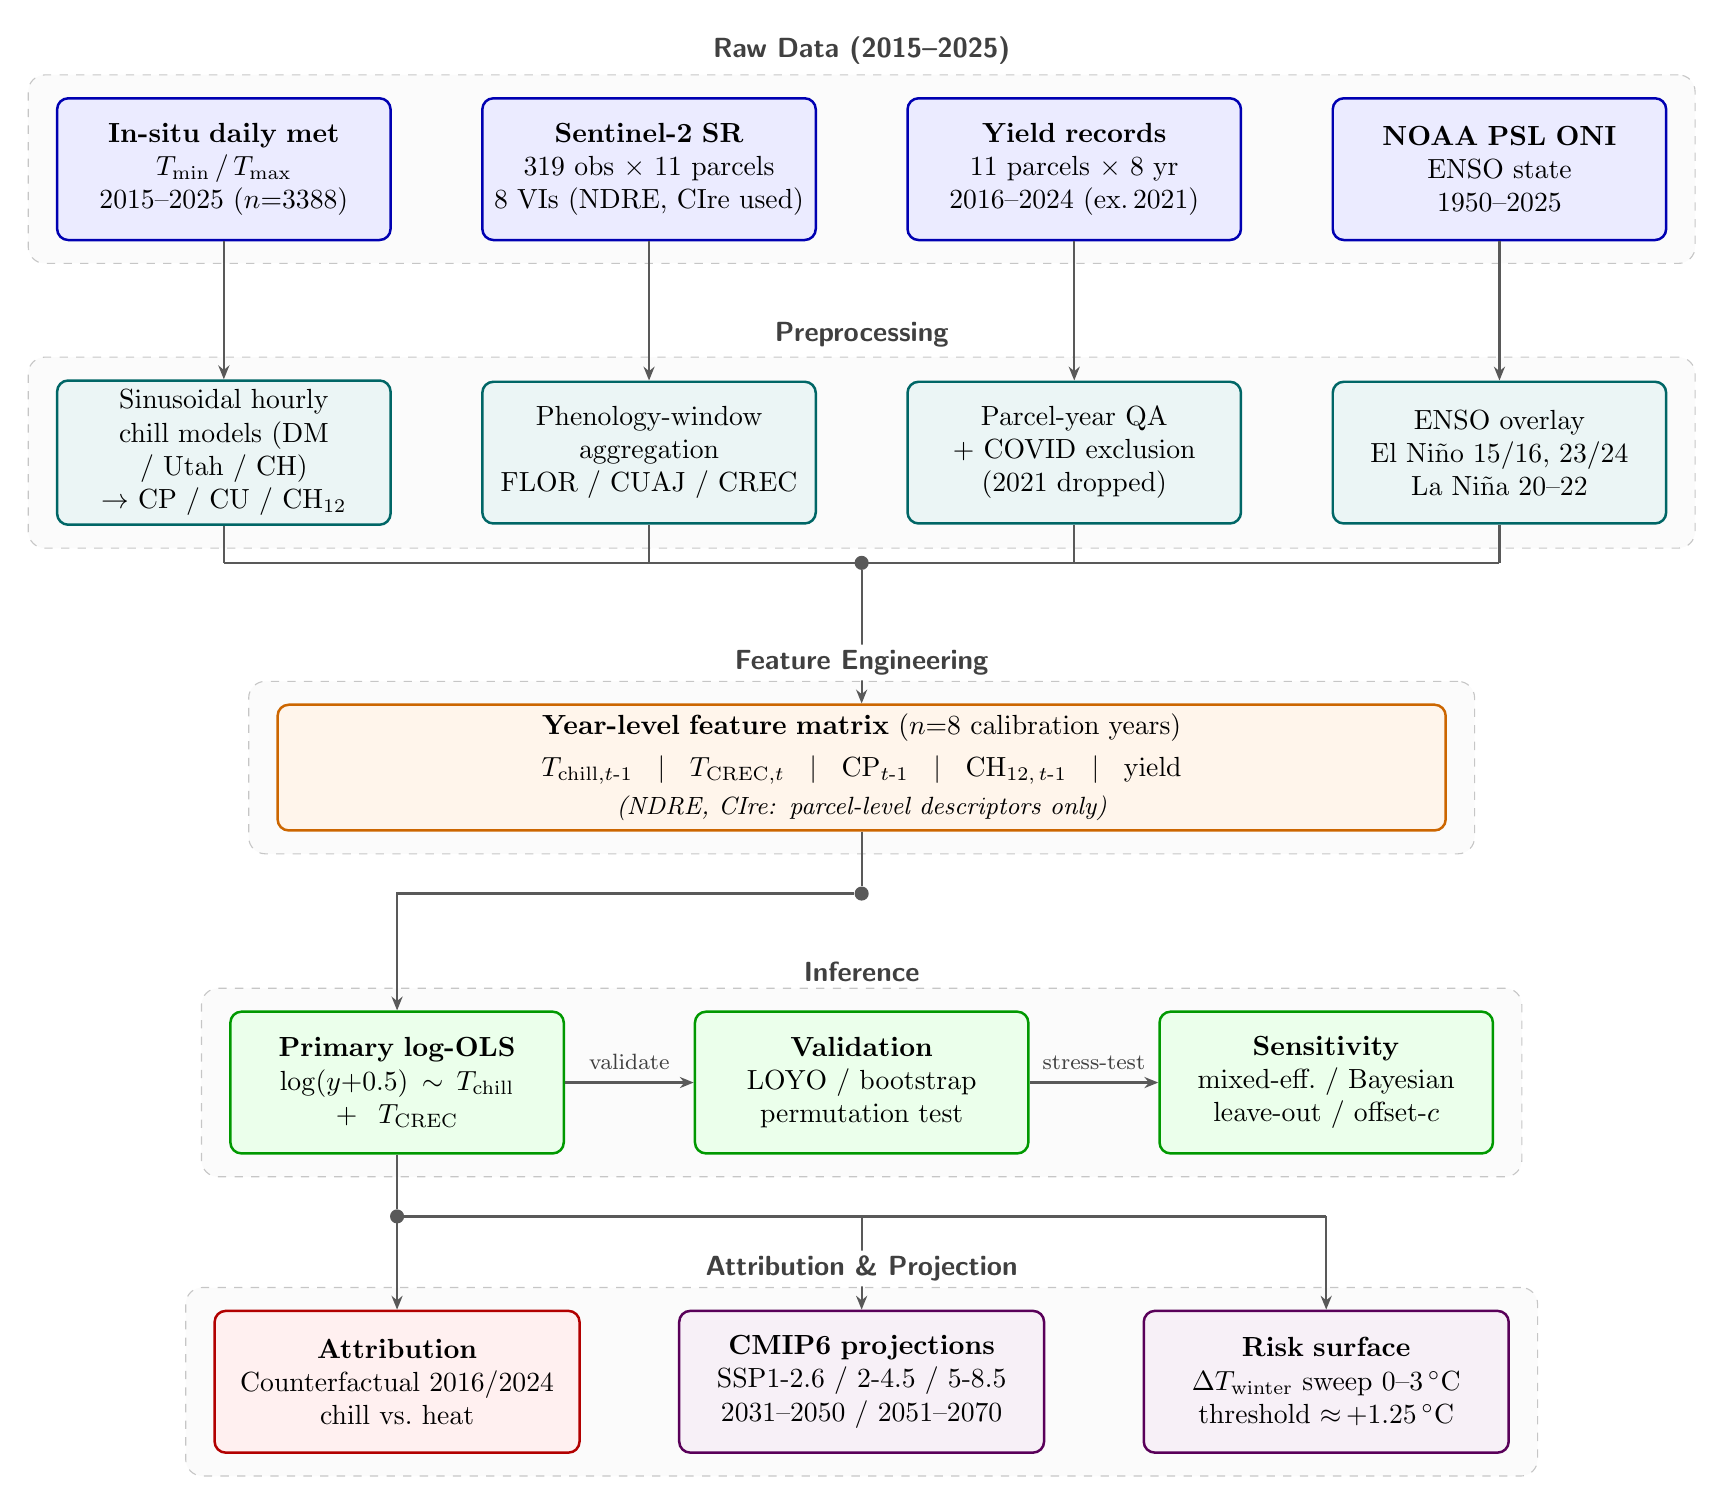
\begin{tikzpicture}[
  % ── Node styles ──────────────────────────────────────────────
  inbox/.style={
    rectangle, rounded corners=4pt, draw=blue!70!black, fill=blue!8,
    line width=0.9pt, text width=4.0cm, minimum height=1.8cm,
    align=center, font=\normalsize},
  procbox/.style={
    rectangle, rounded corners=4pt, draw=teal!80!black, fill=teal!8,
    line width=0.9pt, text width=4.0cm, minimum height=1.8cm,
    align=center, font=\normalsize},
  modbox/.style={
    rectangle, rounded corners=4pt, draw=orange!80!black, fill=orange!8,
    line width=0.9pt, minimum height=1.4cm,
    align=center, font=\normalsize},
  valbox/.style={
    rectangle, rounded corners=4pt, draw=green!60!black, fill=green!8,
    line width=0.9pt, text width=4.0cm, minimum height=1.8cm,
    align=center, font=\normalsize},
  outbox/.style={
    rectangle, rounded corners=4pt, draw=violet!70!black, fill=violet!6,
    line width=0.9pt, text width=4.4cm, minimum height=1.8cm,
    align=center, font=\normalsize},
  % ── Arrow and line styles ───────────────────────────────────
  arr/.style={-{Stealth[length=5pt,width=4pt]}, thick, gray!70!black},
  plainline/.style={thick, gray!70!black},
  % ── Junction dot ─────────────────────────────────────────────
  dot/.style={circle, fill=gray!70!black, inner sep=1.8pt},
  % ── Background group ────────────────────────────────────────
  gbox/.style={draw=gray!45, dashed, rounded corners=6pt,
    inner xsep=10pt, inner ysep=8pt, fill=gray!3},
  glabel/.style={font=\normalsize\bfseries\sffamily, gray!50!black},
  glabelmask/.style={font=\normalsize\bfseries\sffamily, text=gray!50!black,
    fill=white, inner xsep=6pt, inner ysep=2pt, rounded corners=2pt},
]

% ── Column centres (4 columns, evenly spaced) ─────────────────
\def\colA{0}
\def\colB{5.4}
\def\colC{10.8}
\def\colD{16.2}
\pgfmathsetmacro{\gridcenter}{(\colA+\colD)/2}

% =====================================================================
%  ROW 1 — RAW DATA  (y = 0)
% =====================================================================
\node[inbox] (in1) at (\colA,0)
  {\textbf{In-situ daily met}\\
   $T_{\min}$\,/\,$T_{\max}$\\
   2015--2025 ($n{=}3388$)};

\node[inbox] (in2) at (\colB,0)
  {\textbf{Sentinel-2 SR}\\
   319 obs $\times$ 11 parcels\\
   8 VIs (NDRE, CIre used)};

\node[inbox] (in3) at (\colC,0)
  {\textbf{Yield records}\\
   11 parcels $\times$ 8 yr\\
   2016--2024 (ex.\,2021)};

\node[inbox] (in4) at (\colD,0)
  {\textbf{NOAA PSL ONI}\\
   ENSO state\\
   1950--2025};

% =====================================================================
%  ROW 2 — PREPROCESS  (y = -3.6)
% =====================================================================
\node[procbox] (pr1) at (\colA,-3.6)
  {Sinusoidal hourly\\
   chill models (DM / Utah / CH)\\
   $\to$ CP / CU / CH$_{12}$};

\node[procbox] (pr2) at (\colB,-3.6)
  {Phenology-window\\
   aggregation\\
   FLOR / CUAJ / CREC};

\node[procbox] (pr3) at (\colC,-3.6)
  {Parcel-year QA\\
   + COVID exclusion\\
   (2021 dropped)};

\node[procbox] (pr4) at (\colD,-3.6)
  {ENSO overlay\\
   El Ni\~{n}o 15/16, 23/24\\
   La Ni\~{n}a 20--22};

% =====================================================================
%  ROW 3 — FEATURES  (y = -7.6)
% =====================================================================
\node[modbox, text width=14.6cm] (feat) at (\gridcenter,-7.6)
  {\textbf{Year-level feature matrix} ($n{=}8$ calibration years)\\[3pt]
   $T_{\mathrm{chill},t\text{-}1}$ \;\;$\mid$\;\;
   $T_{\mathrm{CREC},t}$ \;\;$\mid$\;\;
   CP$_{t\text{-}1}$ \;\;$\mid$\;\;
   CH$_{12,\,t\text{-}1}$ \;\;$\mid$\;\;
   yield \\[2pt]
   {\small\itshape (NDRE, CIre: parcel-level descriptors only)}};

% =====================================================================
%  ROW 4 — INFERENCE  (y = -11.6)
% =====================================================================
\pgfmathsetmacro{\infA}{\gridcenter - 5.9}
\pgfmathsetmacro{\infB}{\gridcenter}
\pgfmathsetmacro{\infC}{\gridcenter + 5.9}

\node[valbox] (val1) at (\infA,-11.6)
  {\textbf{Primary log-OLS}\\
   $\log(y{+}0.5) \sim T_{\mathrm{chill}}$\\
   $+\; T_{\mathrm{CREC}}$};

\node[valbox] (val2) at (\infB,-11.6)
  {\textbf{Validation}\\
   LOYO / bootstrap\\
   permutation test};

\node[valbox] (val3) at (\infC,-11.6)
  {\textbf{Sensitivity}\\
   mixed-eff.\ / Bayesian\\
   leave-out / offset-$c$};

% =====================================================================
%  ROW 5 — ATTRIBUTION + PROJECTION  (y = -15.4)
% =====================================================================
\pgfmathsetmacro{\attA}{\gridcenter - 5.9}
\pgfmathsetmacro{\attB}{\gridcenter}
\pgfmathsetmacro{\attC}{\gridcenter + 5.9}

\node[outbox, draw=red!70!black, fill=red!6] (cm1) at (\attA,-15.4)
  {\textbf{Attribution}\\
   Counterfactual 2016/2024\\
   chill vs.\ heat};

\node[outbox] (cm2) at (\attB,-15.4)
  {\textbf{CMIP6 projections}\\
   SSP1-2.6 / 2-4.5 / 5-8.5\\
   2031--2050 / 2051--2070};

\node[outbox] (cm3) at (\attC,-15.4)
  {\textbf{Risk surface}\\
   $\Delta T_{\mathrm{winter}}$ sweep 0--3\,$^{\circ}$C\\
   threshold ${\approx}\,{+}1.25\,^{\circ}$C};

% =====================================================================
%  ARROWS — Row 1 → Row 2 (vertical, one-to-one)
% =====================================================================
\draw[arr] (in1) -- (pr1);
\draw[arr] (in2) -- (pr2);
\draw[arr] (in3) -- (pr3);
\draw[arr] (in4) -- (pr4);

% =====================================================================
%  ARROWS — Row 2 → Row 3 (fan-in via horizontal bus)
% =====================================================================
\coordinate (busL) at (\colA,-5.0);
\coordinate (busR) at (\colD,-5.0);
\node[dot] (jin) at (\gridcenter,-5.0) {};

\draw[plainline] (pr1.south) -- (\colA,-5.0);
\draw[plainline] (pr2.south) -- (\colB,-5.0);
\draw[plainline] (pr3.south) -- (\colC,-5.0);
\draw[plainline] (pr4.south) -- (\colD,-5.0);
\draw[plainline] (busL) -- (busR);
\draw[arr] (jin) -- (feat.north);

% =====================================================================
%  ARROWS — Row 3 → Row 4:
%    Feature matrix feeds ONLY the primary OLS (val1). Validation (val2)
%    and sensitivity (val3) operate on the fitted model, not on the raw
%    data, so they receive the flow through val1 via the serial chain
%    below (primary -> validation -> sensitivity, terminating at val3).
% =====================================================================
\node[dot] (jout) at (\gridcenter,-9.2) {};
\draw[plainline] (feat.south) -- (jout);
\draw[arr] (jout) -| (val1.north);

% =====================================================================
%  ARROWS — Row 4 internal (serial assessment chain):
%    val1 (primary OLS) -> val2 (validation) -> val3 (sensitivity).
%    Labels are placed above the arrow with a small yshift and in
%    \footnotesize so they do not touch the adjacent nodes.
% =====================================================================
\draw[arr] (val1.east) -- node[midway, above=1pt, font=\footnotesize, gray!50!black]{validate} (val2.west);
\draw[arr] (val2.east) -- node[midway, above=1pt, font=\footnotesize, gray!50!black]{stress-test} (val3.west);

% =====================================================================
%  ARROWS — Row 4 → Row 5:
%    Only the calibrated OLS (val1) feeds the downstream attribution /
%    projection outputs. A shared bus at y = -13.3 fans out to cm1, cm2, cm3.
% =====================================================================
\coordinate (busvL) at (\infA,-13.3);
\coordinate (busvR) at (\infC,-13.3);
\node[dot] (jdown) at (\infA,-13.3) {};

\draw[plainline] (val1.south) -- (jdown);
\draw[plainline] (busvL) -- (busvR);
\draw[arr] (\infA,-13.3) -- (cm1.north);
\draw[arr] (\infB,-13.3) -- (cm2.north);
\draw[arr] (\infC,-13.3) -- (cm3.north);

% =====================================================================
%  BACKGROUND GROUPS
% =====================================================================
\begin{pgfonlayer}{background}
  \node[gbox, fit=(in1)(in4),
    label={[glabel]above:Raw Data (2015--2025)}] {};
  \node[gbox, fit=(pr1)(pr4),
    label={[glabel]above:Preprocessing}] {};
  \node[gbox, fit=(feat)] (gFeat) {};
  \node[gbox, fit=(val1)(val3)] (gInf) {};
  \node[gbox, fit=(cm1)(cm3)] (gAtt) {};
\end{pgfonlayer}

% Foreground labels with opaque fill so the incoming arrows are masked
% where they cross the label (labels inside pgfonlayer{background} are
% drawn BELOW arrows from the main layer and get visually overwritten).
\node[glabelmask, anchor=south] at (gFeat.north) {Feature Engineering};
\node[glabelmask, anchor=south] at (gInf.north)  {Inference};
\node[glabelmask, anchor=south] at (gAtt.north)  {Attribution \& Projection};

\end{tikzpicture}
}
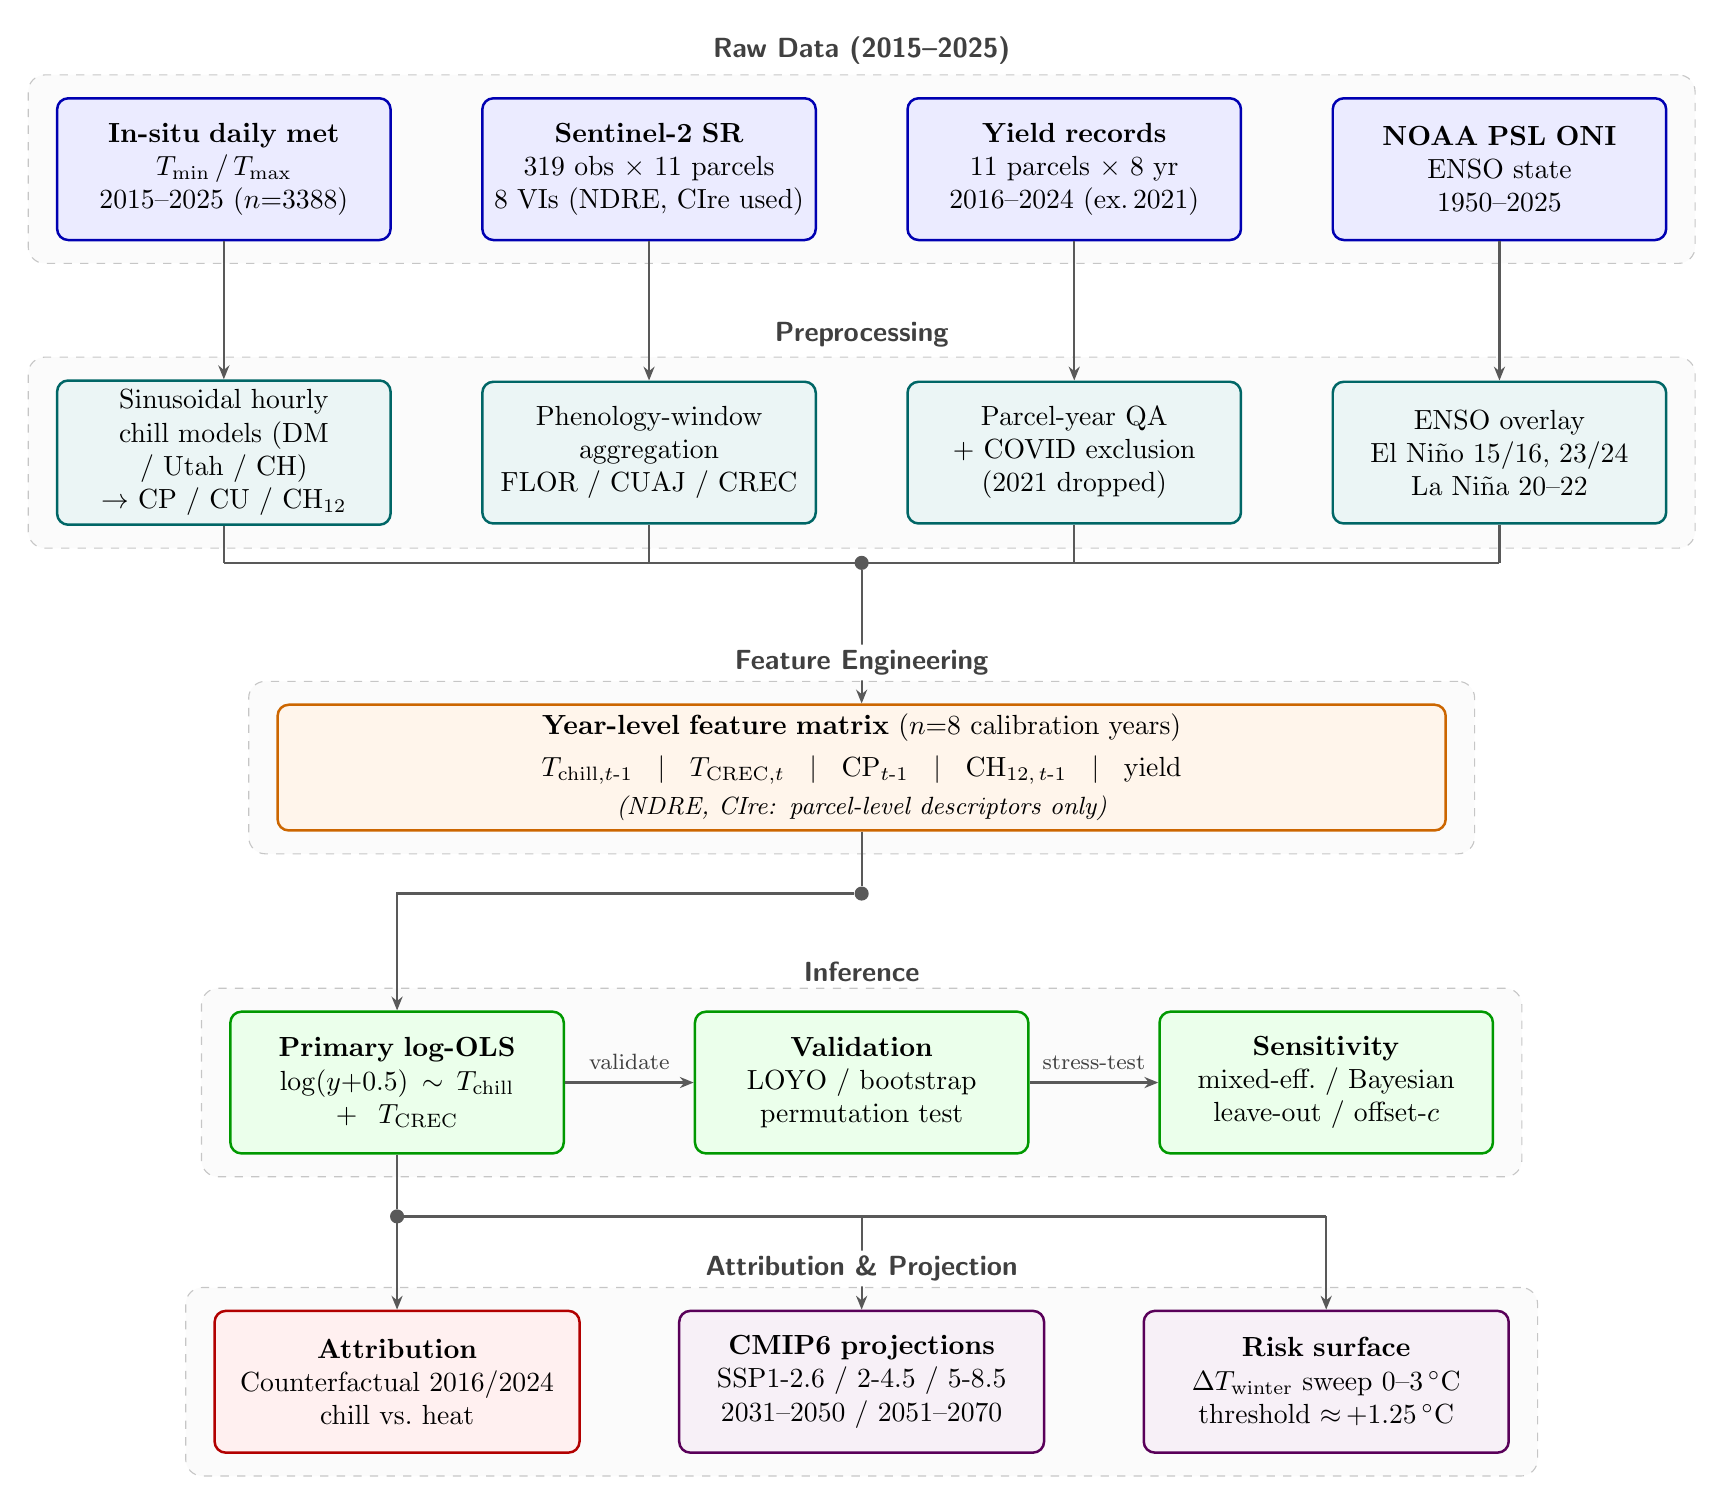
\begin{tikzpicture}[
  % ── Node styles ──────────────────────────────────────────────
  inbox/.style={
    rectangle, rounded corners=4pt, draw=blue!70!black, fill=blue!8,
    line width=0.9pt, text width=4.0cm, minimum height=1.8cm,
    align=center, font=\normalsize},
  procbox/.style={
    rectangle, rounded corners=4pt, draw=teal!80!black, fill=teal!8,
    line width=0.9pt, text width=4.0cm, minimum height=1.8cm,
    align=center, font=\normalsize},
  modbox/.style={
    rectangle, rounded corners=4pt, draw=orange!80!black, fill=orange!8,
    line width=0.9pt, minimum height=1.4cm,
    align=center, font=\normalsize},
  valbox/.style={
    rectangle, rounded corners=4pt, draw=green!60!black, fill=green!8,
    line width=0.9pt, text width=4.0cm, minimum height=1.8cm,
    align=center, font=\normalsize},
  outbox/.style={
    rectangle, rounded corners=4pt, draw=violet!70!black, fill=violet!6,
    line width=0.9pt, text width=4.4cm, minimum height=1.8cm,
    align=center, font=\normalsize},
  % ── Arrow and line styles ───────────────────────────────────
  arr/.style={-{Stealth[length=5pt,width=4pt]}, thick, gray!70!black},
  plainline/.style={thick, gray!70!black},
  % ── Junction dot ─────────────────────────────────────────────
  dot/.style={circle, fill=gray!70!black, inner sep=1.8pt},
  % ── Background group ────────────────────────────────────────
  gbox/.style={draw=gray!45, dashed, rounded corners=6pt,
    inner xsep=10pt, inner ysep=8pt, fill=gray!3},
  glabel/.style={font=\normalsize\bfseries\sffamily, gray!50!black},
  glabelmask/.style={font=\normalsize\bfseries\sffamily, text=gray!50!black,
    fill=white, inner xsep=6pt, inner ysep=2pt, rounded corners=2pt},
]

% ── Column centres (4 columns, evenly spaced) ─────────────────
\def\colA{0}
\def\colB{5.4}
\def\colC{10.8}
\def\colD{16.2}
\pgfmathsetmacro{\gridcenter}{(\colA+\colD)/2}

% =====================================================================
%  ROW 1 — RAW DATA  (y = 0)
% =====================================================================
\node[inbox] (in1) at (\colA,0)
  {\textbf{In-situ daily met}\\
   $T_{\min}$\,/\,$T_{\max}$\\
   2015--2025 ($n{=}3388$)};

\node[inbox] (in2) at (\colB,0)
  {\textbf{Sentinel-2 SR}\\
   319 obs $\times$ 11 parcels\\
   8 VIs (NDRE, CIre used)};

\node[inbox] (in3) at (\colC,0)
  {\textbf{Yield records}\\
   11 parcels $\times$ 8 yr\\
   2016--2024 (ex.\,2021)};

\node[inbox] (in4) at (\colD,0)
  {\textbf{NOAA PSL ONI}\\
   ENSO state\\
   1950--2025};

% =====================================================================
%  ROW 2 — PREPROCESS  (y = -3.6)
% =====================================================================
\node[procbox] (pr1) at (\colA,-3.6)
  {Sinusoidal hourly\\
   chill models (DM / Utah / CH)\\
   $\to$ CP / CU / CH$_{12}$};

\node[procbox] (pr2) at (\colB,-3.6)
  {Phenology-window\\
   aggregation\\
   FLOR / CUAJ / CREC};

\node[procbox] (pr3) at (\colC,-3.6)
  {Parcel-year QA\\
   + COVID exclusion\\
   (2021 dropped)};

\node[procbox] (pr4) at (\colD,-3.6)
  {ENSO overlay\\
   El Ni\~{n}o 15/16, 23/24\\
   La Ni\~{n}a 20--22};

% =====================================================================
%  ROW 3 — FEATURES  (y = -7.6)
% =====================================================================
\node[modbox, text width=14.6cm] (feat) at (\gridcenter,-7.6)
  {\textbf{Year-level feature matrix} ($n{=}8$ calibration years)\\[3pt]
   $T_{\mathrm{chill},t\text{-}1}$ \;\;$\mid$\;\;
   $T_{\mathrm{CREC},t}$ \;\;$\mid$\;\;
   CP$_{t\text{-}1}$ \;\;$\mid$\;\;
   CH$_{12,\,t\text{-}1}$ \;\;$\mid$\;\;
   yield \\[2pt]
   {\small\itshape (NDRE, CIre: parcel-level descriptors only)}};

% =====================================================================
%  ROW 4 — INFERENCE  (y = -11.6)
% =====================================================================
\pgfmathsetmacro{\infA}{\gridcenter - 5.9}
\pgfmathsetmacro{\infB}{\gridcenter}
\pgfmathsetmacro{\infC}{\gridcenter + 5.9}

\node[valbox] (val1) at (\infA,-11.6)
  {\textbf{Primary log-OLS}\\
   $\log(y{+}0.5) \sim T_{\mathrm{chill}}$\\
   $+\; T_{\mathrm{CREC}}$};

\node[valbox] (val2) at (\infB,-11.6)
  {\textbf{Validation}\\
   LOYO / bootstrap\\
   permutation test};

\node[valbox] (val3) at (\infC,-11.6)
  {\textbf{Sensitivity}\\
   mixed-eff.\ / Bayesian\\
   leave-out / offset-$c$};

% =====================================================================
%  ROW 5 — ATTRIBUTION + PROJECTION  (y = -15.4)
% =====================================================================
\pgfmathsetmacro{\attA}{\gridcenter - 5.9}
\pgfmathsetmacro{\attB}{\gridcenter}
\pgfmathsetmacro{\attC}{\gridcenter + 5.9}

\node[outbox, draw=red!70!black, fill=red!6] (cm1) at (\attA,-15.4)
  {\textbf{Attribution}\\
   Counterfactual 2016/2024\\
   chill vs.\ heat};

\node[outbox] (cm2) at (\attB,-15.4)
  {\textbf{CMIP6 projections}\\
   SSP1-2.6 / 2-4.5 / 5-8.5\\
   2031--2050 / 2051--2070};

\node[outbox] (cm3) at (\attC,-15.4)
  {\textbf{Risk surface}\\
   $\Delta T_{\mathrm{winter}}$ sweep 0--3\,$^{\circ}$C\\
   threshold ${\approx}\,{+}1.25\,^{\circ}$C};

% =====================================================================
%  ARROWS — Row 1 → Row 2 (vertical, one-to-one)
% =====================================================================
\draw[arr] (in1) -- (pr1);
\draw[arr] (in2) -- (pr2);
\draw[arr] (in3) -- (pr3);
\draw[arr] (in4) -- (pr4);

% =====================================================================
%  ARROWS — Row 2 → Row 3 (fan-in via horizontal bus)
% =====================================================================
\coordinate (busL) at (\colA,-5.0);
\coordinate (busR) at (\colD,-5.0);
\node[dot] (jin) at (\gridcenter,-5.0) {};

\draw[plainline] (pr1.south) -- (\colA,-5.0);
\draw[plainline] (pr2.south) -- (\colB,-5.0);
\draw[plainline] (pr3.south) -- (\colC,-5.0);
\draw[plainline] (pr4.south) -- (\colD,-5.0);
\draw[plainline] (busL) -- (busR);
\draw[arr] (jin) -- (feat.north);

% =====================================================================
%  ARROWS — Row 3 → Row 4:
%    Feature matrix feeds ONLY the primary OLS (val1). Validation (val2)
%    and sensitivity (val3) operate on the fitted model, not on the raw
%    data, so they receive the flow through val1 via the serial chain
%    below (primary -> validation -> sensitivity, terminating at val3).
% =====================================================================
\node[dot] (jout) at (\gridcenter,-9.2) {};
\draw[plainline] (feat.south) -- (jout);
\draw[arr] (jout) -| (val1.north);

% =====================================================================
%  ARROWS — Row 4 internal (serial assessment chain):
%    val1 (primary OLS) -> val2 (validation) -> val3 (sensitivity).
%    Labels are placed above the arrow with a small yshift and in
%    \footnotesize so they do not touch the adjacent nodes.
% =====================================================================
\draw[arr] (val1.east) -- node[midway, above=1pt, font=\footnotesize, gray!50!black]{validate} (val2.west);
\draw[arr] (val2.east) -- node[midway, above=1pt, font=\footnotesize, gray!50!black]{stress-test} (val3.west);

% =====================================================================
%  ARROWS — Row 4 → Row 5:
%    Only the calibrated OLS (val1) feeds the downstream attribution /
%    projection outputs. A shared bus at y = -13.3 fans out to cm1, cm2, cm3.
% =====================================================================
\coordinate (busvL) at (\infA,-13.3);
\coordinate (busvR) at (\infC,-13.3);
\node[dot] (jdown) at (\infA,-13.3) {};

\draw[plainline] (val1.south) -- (jdown);
\draw[plainline] (busvL) -- (busvR);
\draw[arr] (\infA,-13.3) -- (cm1.north);
\draw[arr] (\infB,-13.3) -- (cm2.north);
\draw[arr] (\infC,-13.3) -- (cm3.north);

% =====================================================================
%  BACKGROUND GROUPS
% =====================================================================
\begin{pgfonlayer}{background}
  \node[gbox, fit=(in1)(in4),
    label={[glabel]above:Raw Data (2015--2025)}] {};
  \node[gbox, fit=(pr1)(pr4),
    label={[glabel]above:Preprocessing}] {};
  \node[gbox, fit=(feat)] (gFeat) {};
  \node[gbox, fit=(val1)(val3)] (gInf) {};
  \node[gbox, fit=(cm1)(cm3)] (gAtt) {};
\end{pgfonlayer}

% Foreground labels with opaque fill so the incoming arrows are masked
% where they cross the label (labels inside pgfonlayer{background} are
% drawn BELOW arrows from the main layer and get visually overwritten).
\node[glabelmask, anchor=south] at (gFeat.north) {Feature Engineering};
\node[glabelmask, anchor=south] at (gInf.north)  {Inference};
\node[glabelmask, anchor=south] at (gAtt.north)  {Attribution \& Projection};

\end{tikzpicture}
}
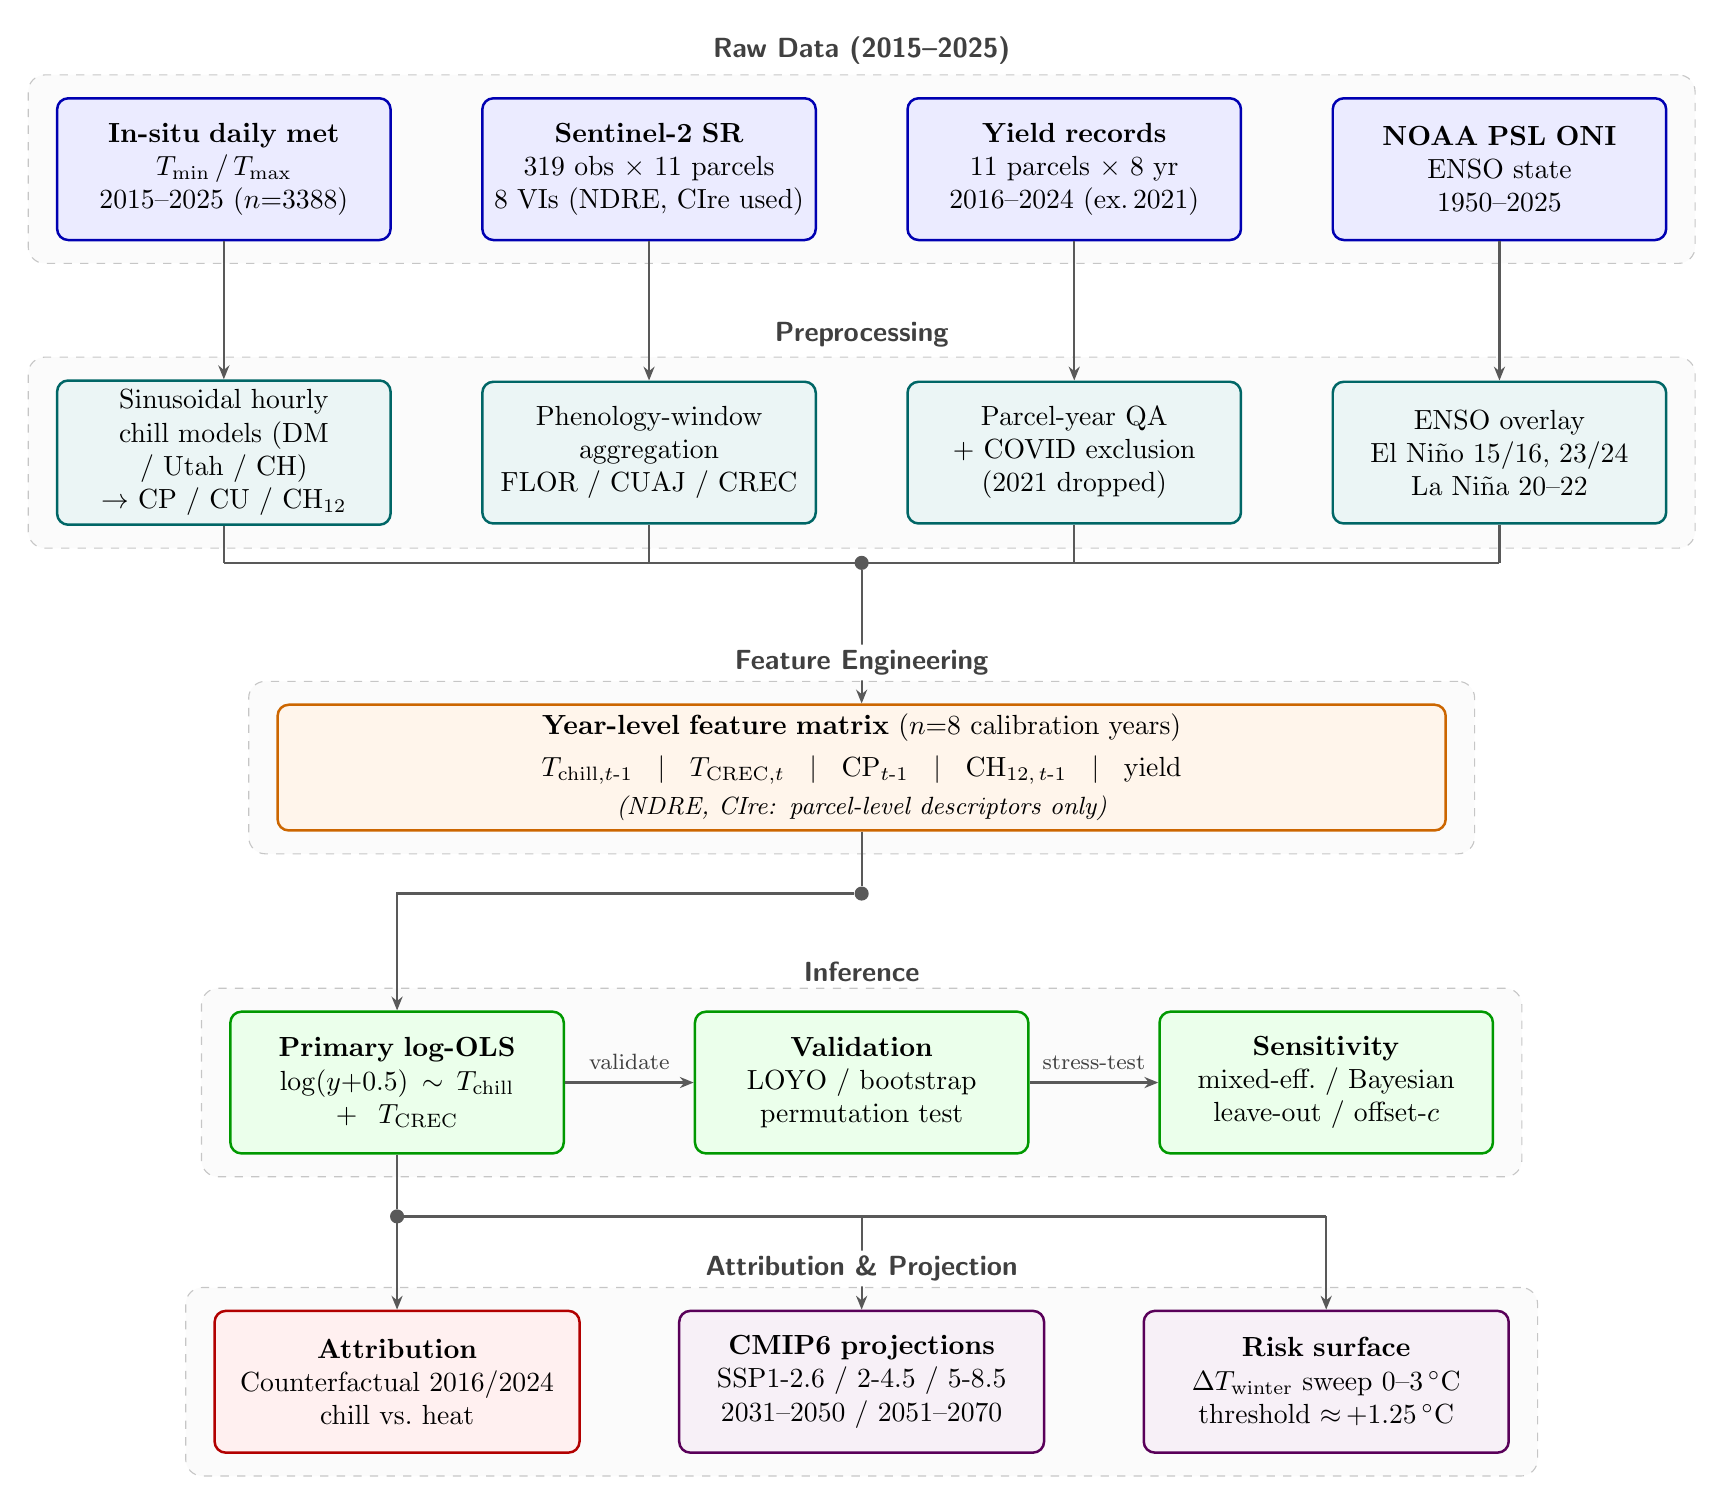
\begin{tikzpicture}[
  % ── Node styles ──────────────────────────────────────────────
  inbox/.style={
    rectangle, rounded corners=4pt, draw=blue!70!black, fill=blue!8,
    line width=0.9pt, text width=4.0cm, minimum height=1.8cm,
    align=center, font=\normalsize},
  procbox/.style={
    rectangle, rounded corners=4pt, draw=teal!80!black, fill=teal!8,
    line width=0.9pt, text width=4.0cm, minimum height=1.8cm,
    align=center, font=\normalsize},
  modbox/.style={
    rectangle, rounded corners=4pt, draw=orange!80!black, fill=orange!8,
    line width=0.9pt, minimum height=1.4cm,
    align=center, font=\normalsize},
  valbox/.style={
    rectangle, rounded corners=4pt, draw=green!60!black, fill=green!8,
    line width=0.9pt, text width=4.0cm, minimum height=1.8cm,
    align=center, font=\normalsize},
  outbox/.style={
    rectangle, rounded corners=4pt, draw=violet!70!black, fill=violet!6,
    line width=0.9pt, text width=4.4cm, minimum height=1.8cm,
    align=center, font=\normalsize},
  % ── Arrow and line styles ───────────────────────────────────
  arr/.style={-{Stealth[length=5pt,width=4pt]}, thick, gray!70!black},
  plainline/.style={thick, gray!70!black},
  % ── Junction dot ─────────────────────────────────────────────
  dot/.style={circle, fill=gray!70!black, inner sep=1.8pt},
  % ── Background group ────────────────────────────────────────
  gbox/.style={draw=gray!45, dashed, rounded corners=6pt,
    inner xsep=10pt, inner ysep=8pt, fill=gray!3},
  glabel/.style={font=\normalsize\bfseries\sffamily, gray!50!black},
  glabelmask/.style={font=\normalsize\bfseries\sffamily, text=gray!50!black,
    fill=white, inner xsep=6pt, inner ysep=2pt, rounded corners=2pt},
]

% ── Column centres (4 columns, evenly spaced) ─────────────────
\def\colA{0}
\def\colB{5.4}
\def\colC{10.8}
\def\colD{16.2}
\pgfmathsetmacro{\gridcenter}{(\colA+\colD)/2}

% =====================================================================
%  ROW 1 — RAW DATA  (y = 0)
% =====================================================================
\node[inbox] (in1) at (\colA,0)
  {\textbf{In-situ daily met}\\
   $T_{\min}$\,/\,$T_{\max}$\\
   2015--2025 ($n{=}3388$)};

\node[inbox] (in2) at (\colB,0)
  {\textbf{Sentinel-2 SR}\\
   319 obs $\times$ 11 parcels\\
   8 VIs (NDRE, CIre used)};

\node[inbox] (in3) at (\colC,0)
  {\textbf{Yield records}\\
   11 parcels $\times$ 8 yr\\
   2016--2024 (ex.\,2021)};

\node[inbox] (in4) at (\colD,0)
  {\textbf{NOAA PSL ONI}\\
   ENSO state\\
   1950--2025};

% =====================================================================
%  ROW 2 — PREPROCESS  (y = -3.6)
% =====================================================================
\node[procbox] (pr1) at (\colA,-3.6)
  {Sinusoidal hourly\\
   chill models (DM / Utah / CH)\\
   $\to$ CP / CU / CH$_{12}$};

\node[procbox] (pr2) at (\colB,-3.6)
  {Phenology-window\\
   aggregation\\
   FLOR / CUAJ / CREC};

\node[procbox] (pr3) at (\colC,-3.6)
  {Parcel-year QA\\
   + COVID exclusion\\
   (2021 dropped)};

\node[procbox] (pr4) at (\colD,-3.6)
  {ENSO overlay\\
   El Ni\~{n}o 15/16, 23/24\\
   La Ni\~{n}a 20--22};

% =====================================================================
%  ROW 3 — FEATURES  (y = -7.6)
% =====================================================================
\node[modbox, text width=14.6cm] (feat) at (\gridcenter,-7.6)
  {\textbf{Year-level feature matrix} ($n{=}8$ calibration years)\\[3pt]
   $T_{\mathrm{chill},t\text{-}1}$ \;\;$\mid$\;\;
   $T_{\mathrm{CREC},t}$ \;\;$\mid$\;\;
   CP$_{t\text{-}1}$ \;\;$\mid$\;\;
   CH$_{12,\,t\text{-}1}$ \;\;$\mid$\;\;
   yield \\[2pt]
   {\small\itshape (NDRE, CIre: parcel-level descriptors only)}};

% =====================================================================
%  ROW 4 — INFERENCE  (y = -11.6)
% =====================================================================
\pgfmathsetmacro{\infA}{\gridcenter - 5.9}
\pgfmathsetmacro{\infB}{\gridcenter}
\pgfmathsetmacro{\infC}{\gridcenter + 5.9}

\node[valbox] (val1) at (\infA,-11.6)
  {\textbf{Primary log-OLS}\\
   $\log(y{+}0.5) \sim T_{\mathrm{chill}}$\\
   $+\; T_{\mathrm{CREC}}$};

\node[valbox] (val2) at (\infB,-11.6)
  {\textbf{Validation}\\
   LOYO / bootstrap\\
   permutation test};

\node[valbox] (val3) at (\infC,-11.6)
  {\textbf{Sensitivity}\\
   mixed-eff.\ / Bayesian\\
   leave-out / offset-$c$};

% =====================================================================
%  ROW 5 — ATTRIBUTION + PROJECTION  (y = -15.4)
% =====================================================================
\pgfmathsetmacro{\attA}{\gridcenter - 5.9}
\pgfmathsetmacro{\attB}{\gridcenter}
\pgfmathsetmacro{\attC}{\gridcenter + 5.9}

\node[outbox, draw=red!70!black, fill=red!6] (cm1) at (\attA,-15.4)
  {\textbf{Attribution}\\
   Counterfactual 2016/2024\\
   chill vs.\ heat};

\node[outbox] (cm2) at (\attB,-15.4)
  {\textbf{CMIP6 projections}\\
   SSP1-2.6 / 2-4.5 / 5-8.5\\
   2031--2050 / 2051--2070};

\node[outbox] (cm3) at (\attC,-15.4)
  {\textbf{Risk surface}\\
   $\Delta T_{\mathrm{winter}}$ sweep 0--3\,$^{\circ}$C\\
   threshold ${\approx}\,{+}1.25\,^{\circ}$C};

% =====================================================================
%  ARROWS — Row 1 → Row 2 (vertical, one-to-one)
% =====================================================================
\draw[arr] (in1) -- (pr1);
\draw[arr] (in2) -- (pr2);
\draw[arr] (in3) -- (pr3);
\draw[arr] (in4) -- (pr4);

% =====================================================================
%  ARROWS — Row 2 → Row 3 (fan-in via horizontal bus)
% =====================================================================
\coordinate (busL) at (\colA,-5.0);
\coordinate (busR) at (\colD,-5.0);
\node[dot] (jin) at (\gridcenter,-5.0) {};

\draw[plainline] (pr1.south) -- (\colA,-5.0);
\draw[plainline] (pr2.south) -- (\colB,-5.0);
\draw[plainline] (pr3.south) -- (\colC,-5.0);
\draw[plainline] (pr4.south) -- (\colD,-5.0);
\draw[plainline] (busL) -- (busR);
\draw[arr] (jin) -- (feat.north);

% =====================================================================
%  ARROWS — Row 3 → Row 4:
%    Feature matrix feeds ONLY the primary OLS (val1). Validation (val2)
%    and sensitivity (val3) operate on the fitted model, not on the raw
%    data, so they receive the flow through val1 via the serial chain
%    below (primary -> validation -> sensitivity, terminating at val3).
% =====================================================================
\node[dot] (jout) at (\gridcenter,-9.2) {};
\draw[plainline] (feat.south) -- (jout);
\draw[arr] (jout) -| (val1.north);

% =====================================================================
%  ARROWS — Row 4 internal (serial assessment chain):
%    val1 (primary OLS) -> val2 (validation) -> val3 (sensitivity).
%    Labels are placed above the arrow with a small yshift and in
%    \footnotesize so they do not touch the adjacent nodes.
% =====================================================================
\draw[arr] (val1.east) -- node[midway, above=1pt, font=\footnotesize, gray!50!black]{validate} (val2.west);
\draw[arr] (val2.east) -- node[midway, above=1pt, font=\footnotesize, gray!50!black]{stress-test} (val3.west);

% =====================================================================
%  ARROWS — Row 4 → Row 5:
%    Only the calibrated OLS (val1) feeds the downstream attribution /
%    projection outputs. A shared bus at y = -13.3 fans out to cm1, cm2, cm3.
% =====================================================================
\coordinate (busvL) at (\infA,-13.3);
\coordinate (busvR) at (\infC,-13.3);
\node[dot] (jdown) at (\infA,-13.3) {};

\draw[plainline] (val1.south) -- (jdown);
\draw[plainline] (busvL) -- (busvR);
\draw[arr] (\infA,-13.3) -- (cm1.north);
\draw[arr] (\infB,-13.3) -- (cm2.north);
\draw[arr] (\infC,-13.3) -- (cm3.north);

% =====================================================================
%  BACKGROUND GROUPS
% =====================================================================
\begin{pgfonlayer}{background}
  \node[gbox, fit=(in1)(in4),
    label={[glabel]above:Raw Data (2015--2025)}] {};
  \node[gbox, fit=(pr1)(pr4),
    label={[glabel]above:Preprocessing}] {};
  \node[gbox, fit=(feat)] (gFeat) {};
  \node[gbox, fit=(val1)(val3)] (gInf) {};
  \node[gbox, fit=(cm1)(cm3)] (gAtt) {};
\end{pgfonlayer}

% Foreground labels with opaque fill so the incoming arrows are masked
% where they cross the label (labels inside pgfonlayer{background} are
% drawn BELOW arrows from the main layer and get visually overwritten).
\node[glabelmask, anchor=south] at (gFeat.north) {Feature Engineering};
\node[glabelmask, anchor=south] at (gInf.north)  {Inference};
\node[glabelmask, anchor=south] at (gAtt.north)  {Attribution \& Projection};

\end{tikzpicture}
}
\caption{Five-tier analytical workflow for chill-window attribution of olive yield collapse at the Tacna coast: raw inputs (row~1) $\to$ preprocessing (row~2) $\to$ year-level feature matrix (row~3; Table~\ref{tab:year_level}, $n=8$) $\to$ inference (row~4: primary log-OLS of Eq.~\eqref{eq:primary}, validation, sensitivity) $\to$ attribution and projection (row~5: 2016/2024 counterfactual, CMIP6 SSP projections for 2031--2070, $\Delta T_{\text{winter}}$ risk surface).\label{fig:workflow}}
\end{figure}

%=================================================================
\section{Results}
\label{sec:results}

\subsection{ENSO--Chill--Yield Correspondence}
\label{sec:results_enso}

Figure~\ref{fig:enso_overlay} aligns the eight observed harvest seasons with the corresponding chill-window meteorology and the NOAA ONI. The two failure seasons (2016, harvest 1.60~t~ha$^{-1}$; 2024, harvest 0.68~t~ha$^{-1}$) follow the two strongest El~Ni\~{n}o events of the satellite era (2015/16 and 2023/24), which lifted the May--August $T_{\text{mean}}$ of the preceding chill window from a non-failure climatology of $\approx 16.7\,^\circ$C to $18.2\,^\circ$C (chill year 2015) and $18.5\,^\circ$C (chill year 2023). Conversely the bumper season of 2022 (12.06~t~ha$^{-1}$) follows the central year of the 2020--2022 triple La~Ni\~{n}a, with $T_{\text{chill}}$ of the 2021 winter at $16.6\,^\circ$C. The visual correspondence is essentially binary: every El-Ni\~{n}o-warmed winter is followed by a failure season, and every cool winter is followed by a productive season. CP under the Dynamic Model collapses to exactly zero in five of the eight chill years, including both failure years, but the floor effect means that CP does not by itself separate the two failure years from the moderate-yield years 2017 and 2018 --- only $T_{\text{chill}}$ does (Section~\ref{sec:results_corr}).

\begin{figure}[H]
\centering
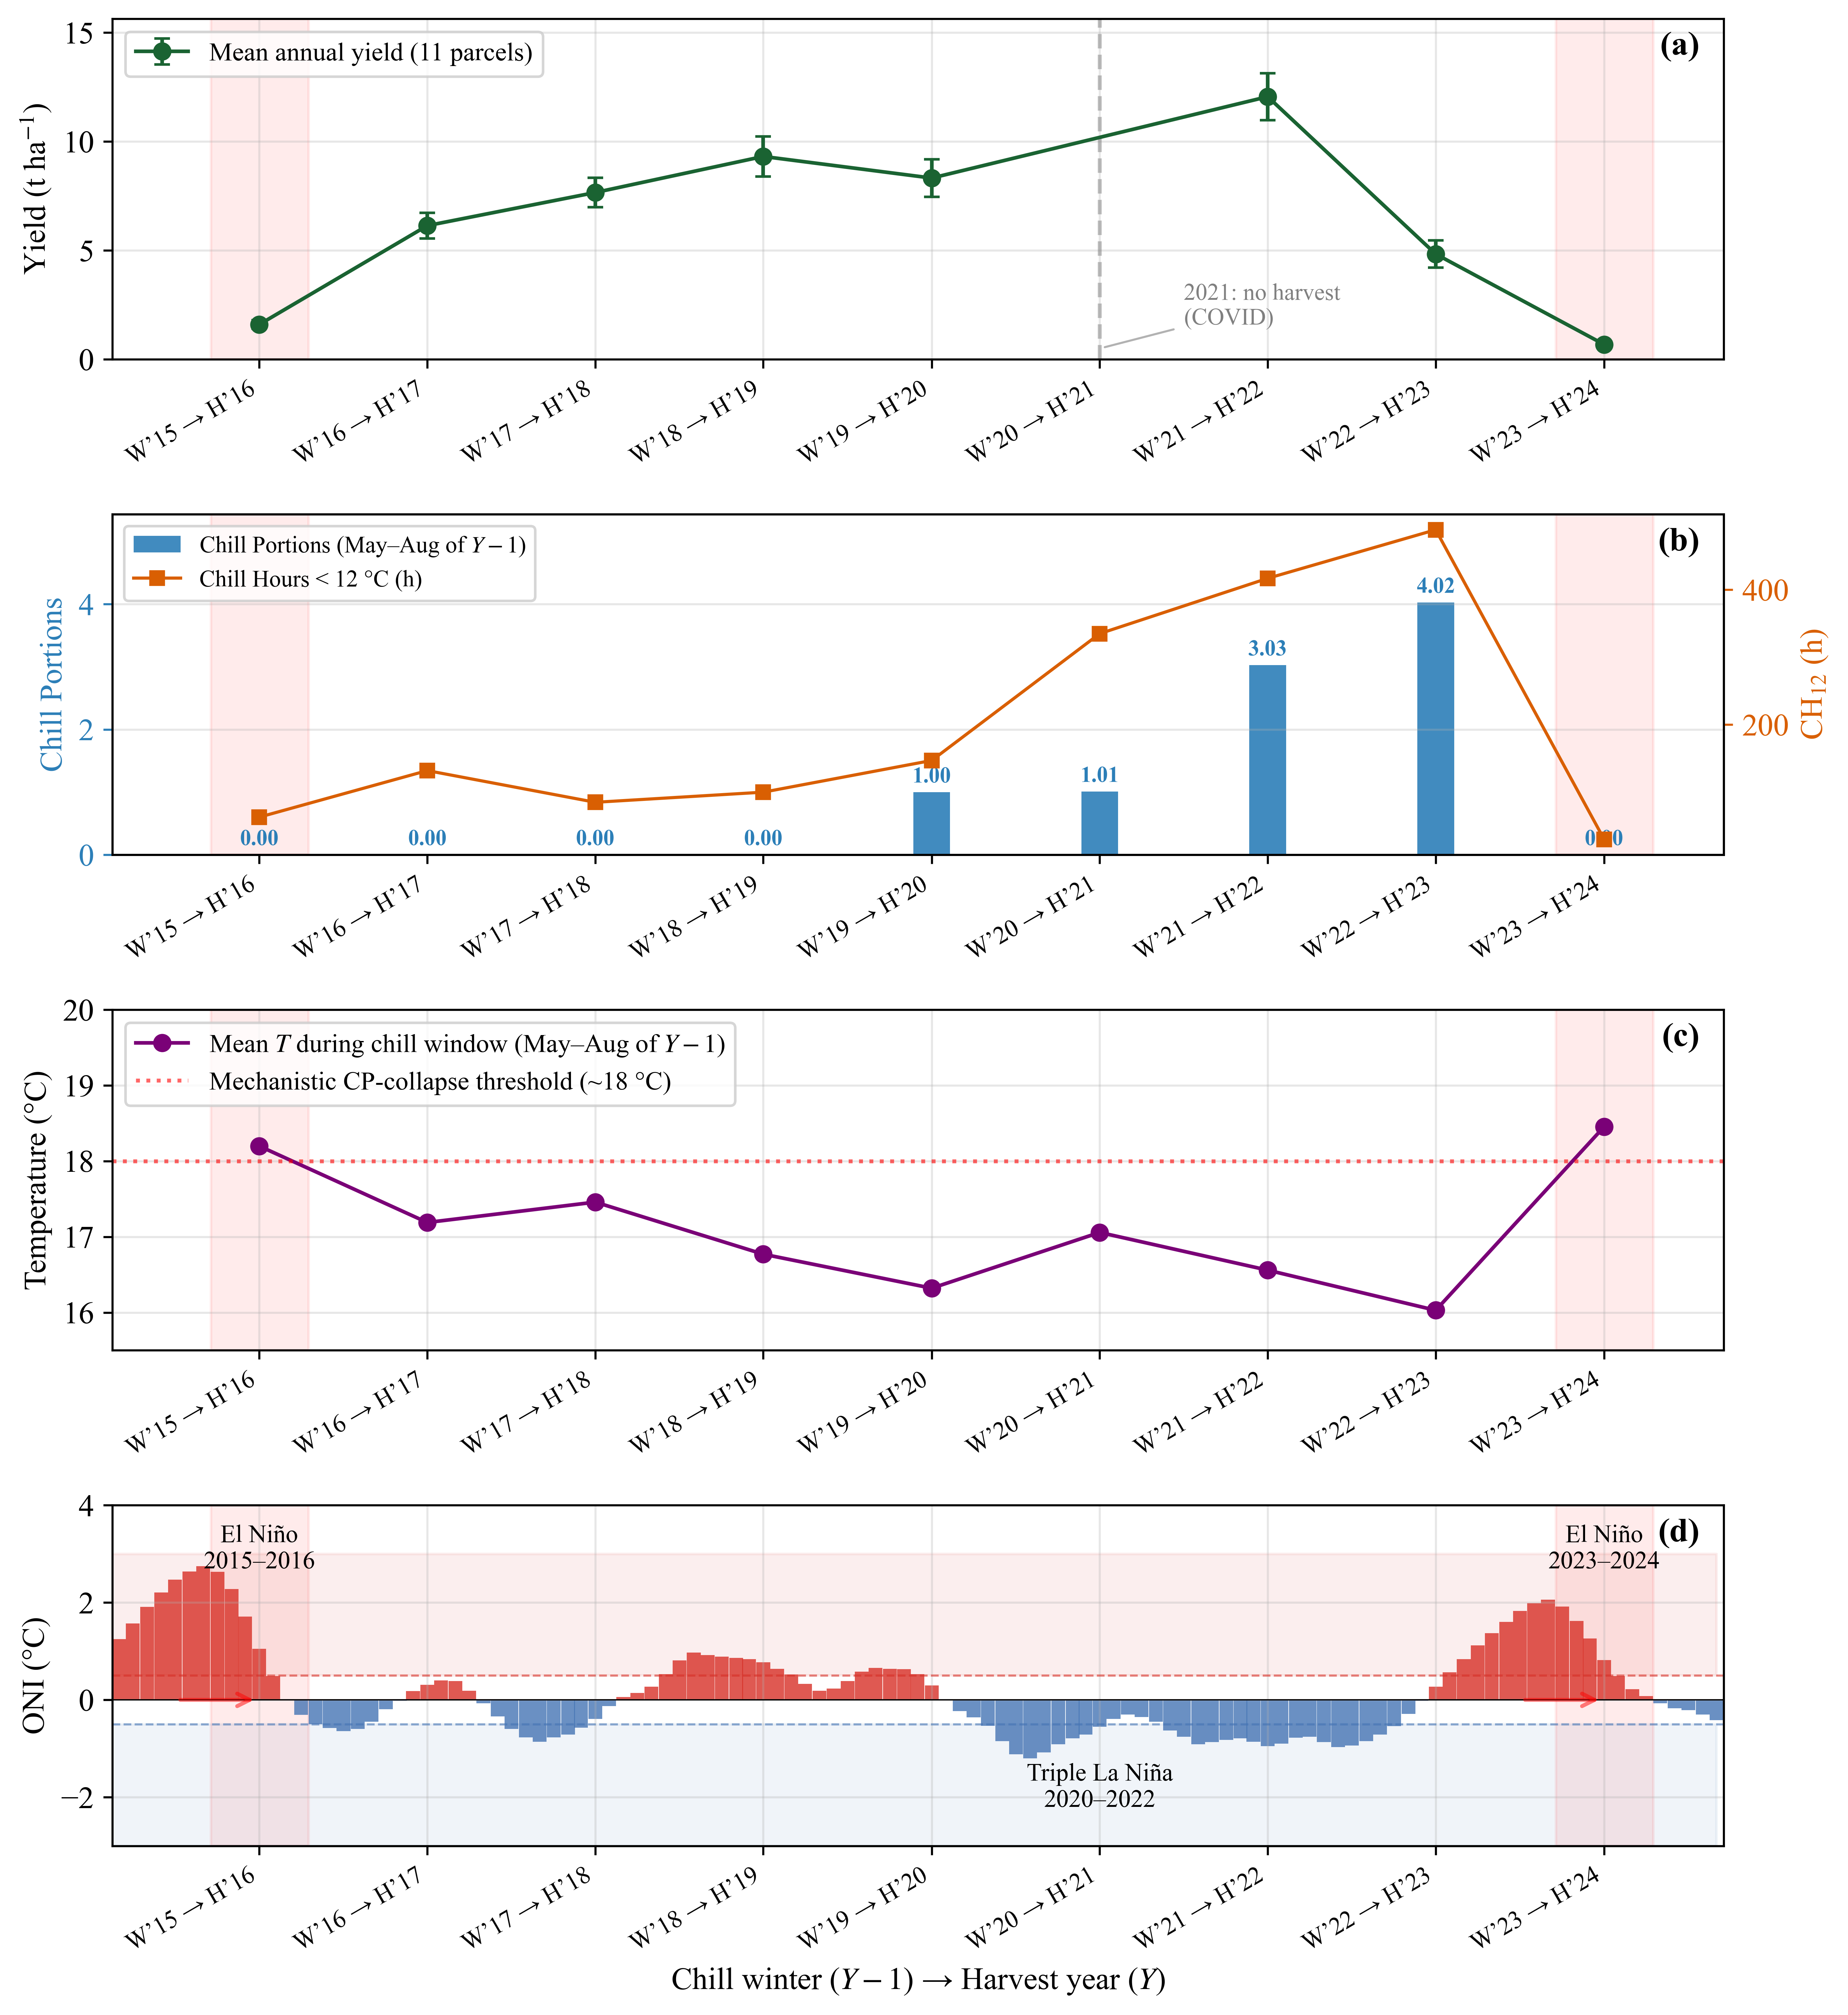
\includegraphics[width=\textwidth]{Figure4.png}
\caption{ENSO~$\to$~chill~$\to$~yield chain in Tacna 2015--2025. (\textbf{a})~Annual mean olive yield $\pm$~SD across 11 parcels (plotted at the harvest year $Y$); the 2021 harvest is missing because of COVID-19 (no harvest campaign). (\textbf{b})~Chill Portions and Chill Hours $<12\,^\circ$C (May--August of the chill year $Y-1$, Dynamic Model); note that the chill accumulation plotted at year $Y-1$ determines the yield plotted at year $Y$ in panel~(a). (\textbf{c})~Mean chill-window air temperature ($Y-1$). The dashed horizontal line at $\sim 18\,^\circ$C is the model-derived chill-collapse threshold corresponding to $\Delta T_{\text{winter}}\approx +1.25\,^\circ$C above the non-failure climatology, at which Chill Portions under the Dynamic Model reach zero (Figure~\ref{fig:warming_sweep} and Supplementary Figure~\ref{fig:S4}); it is shown here as a visual reference rather than as an externally calibrated threshold. (\textbf{d})~NOAA PSL Oceanic Ni\~{n}o Index. Red shading marks the 2016 and 2024 failure seasons and connects each warm winter ($Y-1$) to its subsequent yield collapse ($Y$).\label{fig:enso_overlay}}
\end{figure}

\subsection{Year-Level Correlation Structure}
\label{sec:results_corr}

At the year level, the strongest single-predictor correlation with observed yield is $T_{\text{chill},t-1}$ ($r=-0.697$), which is substantially larger in absolute value than any heat-side predictor: $T_{\max,\text{FLOR}}$ ($r=-0.492$), CH$_{12,t-1}$ ($r=+0.404$), $T_{\text{mean},\text{FLOR}}$ ($r=-0.381$), $T_{\max,\text{CREC}}$ ($r=-0.375$), $T_{\text{CREC},t}$ ($r=-0.313$), CP$_{t-1}$ ($r=+0.307$), and ET$_{0,\text{CREC}}$ ($r=-0.178$); the full table is in Supplementary Table~\ref{tab:year_corr}. The reason CP underperforms is not that it is wrong physically --- it is the canonical Mediterranean chill metric --- but that it floors at zero in five of eight years, losing resolution exactly in the warm tail where the attribution question lives.

The pair $\{T_{\text{chill},t-1},\,T_{\text{CREC},t}\}$ was selected as the primary predictor pair on the basis of (i)~$T_{\text{chill},t-1}$ being the dominant single predictor, (ii)~$T_{\text{CREC},t}$ representing the physiologically distinct fruit-growth heat channel, enabling a clean chill-vs-heat counterfactual decomposition, and (iii)~$T_{\text{CREC},t}$ showing the lowest collinearity with the chill predictor among all candidate heat-side variables (year-level $r(T_{\text{chill}},\,T_{\text{CREC}})=0.409$, against $r=0.452$ for $T_{\max,\text{FLOR}}$ and $r=0.571$ for $T_{\text{mean},\text{FLOR}}$). Although this moderate correlation is larger than a strict orthogonality assumption would require --- both warm ENSO winters and the subsequent austral summers tend to sit slightly above the regional thermal baseline --- the variance inflation factor of the two-predictor model remains below~2, and the chill coefficient changes magnitude and significance only modestly when $T_{\text{CREC},t}$ is removed (Section~\ref{sec:results_robust}), so the pair is statistically stable.

\subsection{Primary Attribution Model}
\label{sec:results_primary}

The fitted log-OLS model (Table~\ref{tab:primary_coef}) explains 65.3\,\% of the inter-annual variance in log-yield (adjusted $R^{2}=0.514$, $F(2,5)=4.70$, $p=0.071$). $T_{\text{chill},t-1}$ is the dominant predictor with $\beta=-0.816$ (SE $0.272$, $p=0.030$): each $1\,^\circ$C of warming in the chill window of the preceding austral winter reduces $\log(\text{yield}+0.5)$ by 0.82, which corresponds to a multiplicative factor of $\exp(-0.82)\approx 0.44$ on yield in the heart of the response curve. $T_{\text{CREC},t}$ enters with a small positive coefficient that is statistically indistinguishable from zero ($\beta=+0.089$, SE $0.131$, $p=0.53$); we retain it in the model because it allows the clean chill-vs-heat decomposition in the counterfactual analysis (Section~\ref{sec:results_counterfactual}), and because it is the predictor that operationalises the orthogonal-to-chill fruit-growth window (Section~\ref{sec:results_corr}). Its near-zero estimate on the Humboldt-cooled coast is itself an informative finding: summer heat stress is not the binding constraint at this site over the calibration sample.

Back-transformed in-sample $R^{2}$ on the raw t~ha$^{-1}$ scale is $0.108$, RMSE $3.41$~t~ha$^{-1}$, MAE $2.54$~t~ha$^{-1}$; the gap between the log-space and raw-scale $R^{2}$ reflects the non-linearity of the back-transformation and the leverage of the extreme years (the bumper 2022 harvest and the two failure years drive a large share of raw-scale variance). The 5000-iteration permutation test gives a two-sided $p=0.072$ (observed $R^{2}_{\log}=0.653$; null mean $0.285$; 95th null percentile $0.701$); because the physiological hypothesis is strictly directional (warmer chill windows reduce yield), the corresponding one-sided $p$ is $0.036$. The partial chill effect of $T_{\text{chill},t-1}$, holding $T_{\text{CREC},t}$ at its sample mean, is shown in Supplementary Figure~\ref{fig:S2}; residual diagnostics (normality, homoscedasticity, leverage) of the fitted model are shown in Supplementary Figure~\ref{fig:S5}.

\paragraph{Three independent lines of evidence for a negative chill coefficient.} Because the year-level sample is small ($n=8$, five residual degrees of freedom) we assessed the robustness of the chill signal under three methodologically independent tests, reported in full in Supplementary Section on robustness and summarised here.
\emph{Line 1 --- frequentist.} The OLS slope $\beta_{T_{\text{chill}}}=-0.816$ has a one-sided analytic $p=0.015$ (half of the two-sided $t$-test $p=0.030$ reported above, applicable under the directional physiological hypothesis that warmer chill windows reduce yield), and the 5000-iteration year-block permutation test gives a one-sided $p=0.036$ against the same directional null; both are below conventional 5\,\%.
\emph{Line 2 --- Bayesian.} Under a weakly-informative $N(0,1)$ prior on the standardised slope, the closed-form posterior of the chill slope on the natural scale is $N(-0.775,\,0.264)$ (Supplementary Figure~\ref{fig:S8}), with $\Pr(\beta_{T_{\text{chill}}}<0 \mid \text{data})=0.998$. The Savage--Dickey Bayes factor against the two-sided null is BF$_{10}=15.9$ (strong evidence on the Kass--Raftery scale), and the one-sided Bayes factor in favour of $\beta<0$ relative to $\beta\geq 0$ is $\sim 5.9\times 10^{2}$.
\emph{Line 3 --- parcel-year hierarchical.} A random-intercept linear mixed-effects model fitted on the full 88-parcel-year matrix (11 parcels $\times$ 8 seasons) with standardised climate predictors gives a chill slope of $\beta_{T_{\text{chill}}}^{\text{std}}=-2.48$ (SE $0.32$, $z=-7.78$, $p<10^{-14}$, two-sided), with an ICC at the parcel level of $\approx 0$ confirming that parcels within this homogeneous orchard are statistically exchangeable and that the year is the appropriate inferential unit. A post-hoc Monte-Carlo power calculation indicates that the observed effect size and residual variance would already be detectable at one-sided $\alpha=0.05$ with four seasons of data, so the sign and magnitude of the chill effect are not sample-size-limited.
All three tests converge on the same sign, a magnitude compatible with a $\sim 45\,\%$ multiplicative reduction in yield per $1\,^{\circ}$C of chill-window warming ($\exp(-0.82)\approx 0.44$ through the heart of the response), and significance at or below the conventional 5\,\% level. We therefore treat the negative chill coefficient as a robust finding and not an artefact of a marginal two-sided $p$-value at $n=8$.

% Table 2 — Primary log-OLS coefficients
\begin{table}[H]
\caption{Primary attribution model coefficients. Model: $\log(y_{t}+0.5) = \beta_{0} + \beta_{1}\,T_{\text{chill},t-1} + \beta_{2}\,T_{\text{CREC},t} + \varepsilon_{t}$, fitted at the year level ($n=8$). 95\,\% CIs and bootstrap two-sided $p$-values come from a 5000-iteration year-block bootstrap. Predictor collinearity and permutation-test details are reported in Section~\ref{sec:results_primary}.\label{tab:primary_coef}}
\centering
\footnotesize
\setlength{\tabcolsep}{4pt}
\begin{tabular}{lcccccc}
\toprule
\textbf{Term} & \textbf{Estimate} & \textbf{SE} & \textbf{$t$} & \textbf{$p$ (OLS)} & \textbf{95\,\% CI} & \textbf{$p$ (boot)} \\
\midrule
Intercept                & $+13.768$ & $4.350$ & $+3.165$ & $0.0249$         & $[2.587,\,24.949]$  & ---     \\
$T_{\text{chill},t-1}$   & $-0.816$  & $0.272$ & $-3.004$ & $\mathbf{0.030}$ & $[-1.515,\,-0.118]$ & $0.171$ \\
$T_{\text{CREC},t}$      & $+0.089$  & $0.131$ & $+0.675$ & $0.5294$         & $[-0.249,\,+0.427]$ & $0.573$ \\
\bottomrule
\end{tabular}

\vspace{4pt}
\footnotesize
\noindent\textit{Goodness of fit (log space):} $R^{2}=0.653$; adj.\ $R^{2}=0.514$; $F(2,5)=4.70$; $p=0.071$. \\
\textit{Back-transformed (raw t~ha$^{-1}$):} $R^{2}=0.108$; RMSE $=3.41$; MAE $=2.54$. \\
\textit{LOYO cross-validation:} $R^{2}_{\log}=-0.07$; $R^{2}_{\text{back}}=-1.69$; RMSE $=5.92$~t~ha$^{-1}$. \\
\textit{Single-predictor sensitivity} ($T_{\text{chill},t-1}$ only): $R^{2}_{\log}=0.621$; $F(1,6)=9.83$; $p=0.020$; $\beta=-0.741\pm0.236$.
\end{table}


\subsection{Cross-Validation and Robustness}
\label{sec:results_robust}

LOYO cross-validation is weak: $R^{2}_{\log}=-0.07$ and back-transformation gives $R^{2}=-1.69$ with RMSE $5.92$~t~ha$^{-1}$ (Figure~\ref{fig:loyo}). With $n=8$ years, every single hold-out fold removes $12.5\,\%$ of the sample and forces the model to extrapolate into a region of predictor space that is not represented in the training fold: the 2022 bumper year is under-predicted (LOYO $3.28$ vs observed $12.06$~t~ha$^{-1}$) and the 2023 harvest is over-predicted (LOYO $17.82$ vs observed $4.84$~t~ha$^{-1}$) because removing the centre of the chill-predictor distribution unanchors the slope.

The failure years are nevertheless placed in the lower half of the LOYO predicted distribution (2016: $2.64$~t~ha$^{-1}$, rank 2 of 8; 2024: $3.13$~t~ha$^{-1}$, rank 4 of 8 under LOYO), so the collapse signal is recovered in rank terms even though the quantitative LOYO skill is poor. The single-predictor variant $\log(y+0.5)\sim T_{\text{chill},t-1}$ is actually the more defensible parsimonious formulation: its in-sample fit ($R^{2}_{\log}=0.621$, $F(1,6)=9.83$, $p=0.020$; $\beta=-0.741$, SE $0.236$) crosses the conventional significance threshold that the two-predictor $F$-test narrowly misses, confirming that the chill side of the model is the load-bearing piece. We therefore emphasise that LOYO with $n=8$ is a severely conservative robustness check --- it is not a forecast skill test --- and that the primary empirical evidence for chill attribution rests on the in-sample coefficient estimate, its year-block bootstrap envelope, and the counterfactual decomposition that follows, rather than on LOYO predictive accuracy.

\begin{figure}[H]
\centering
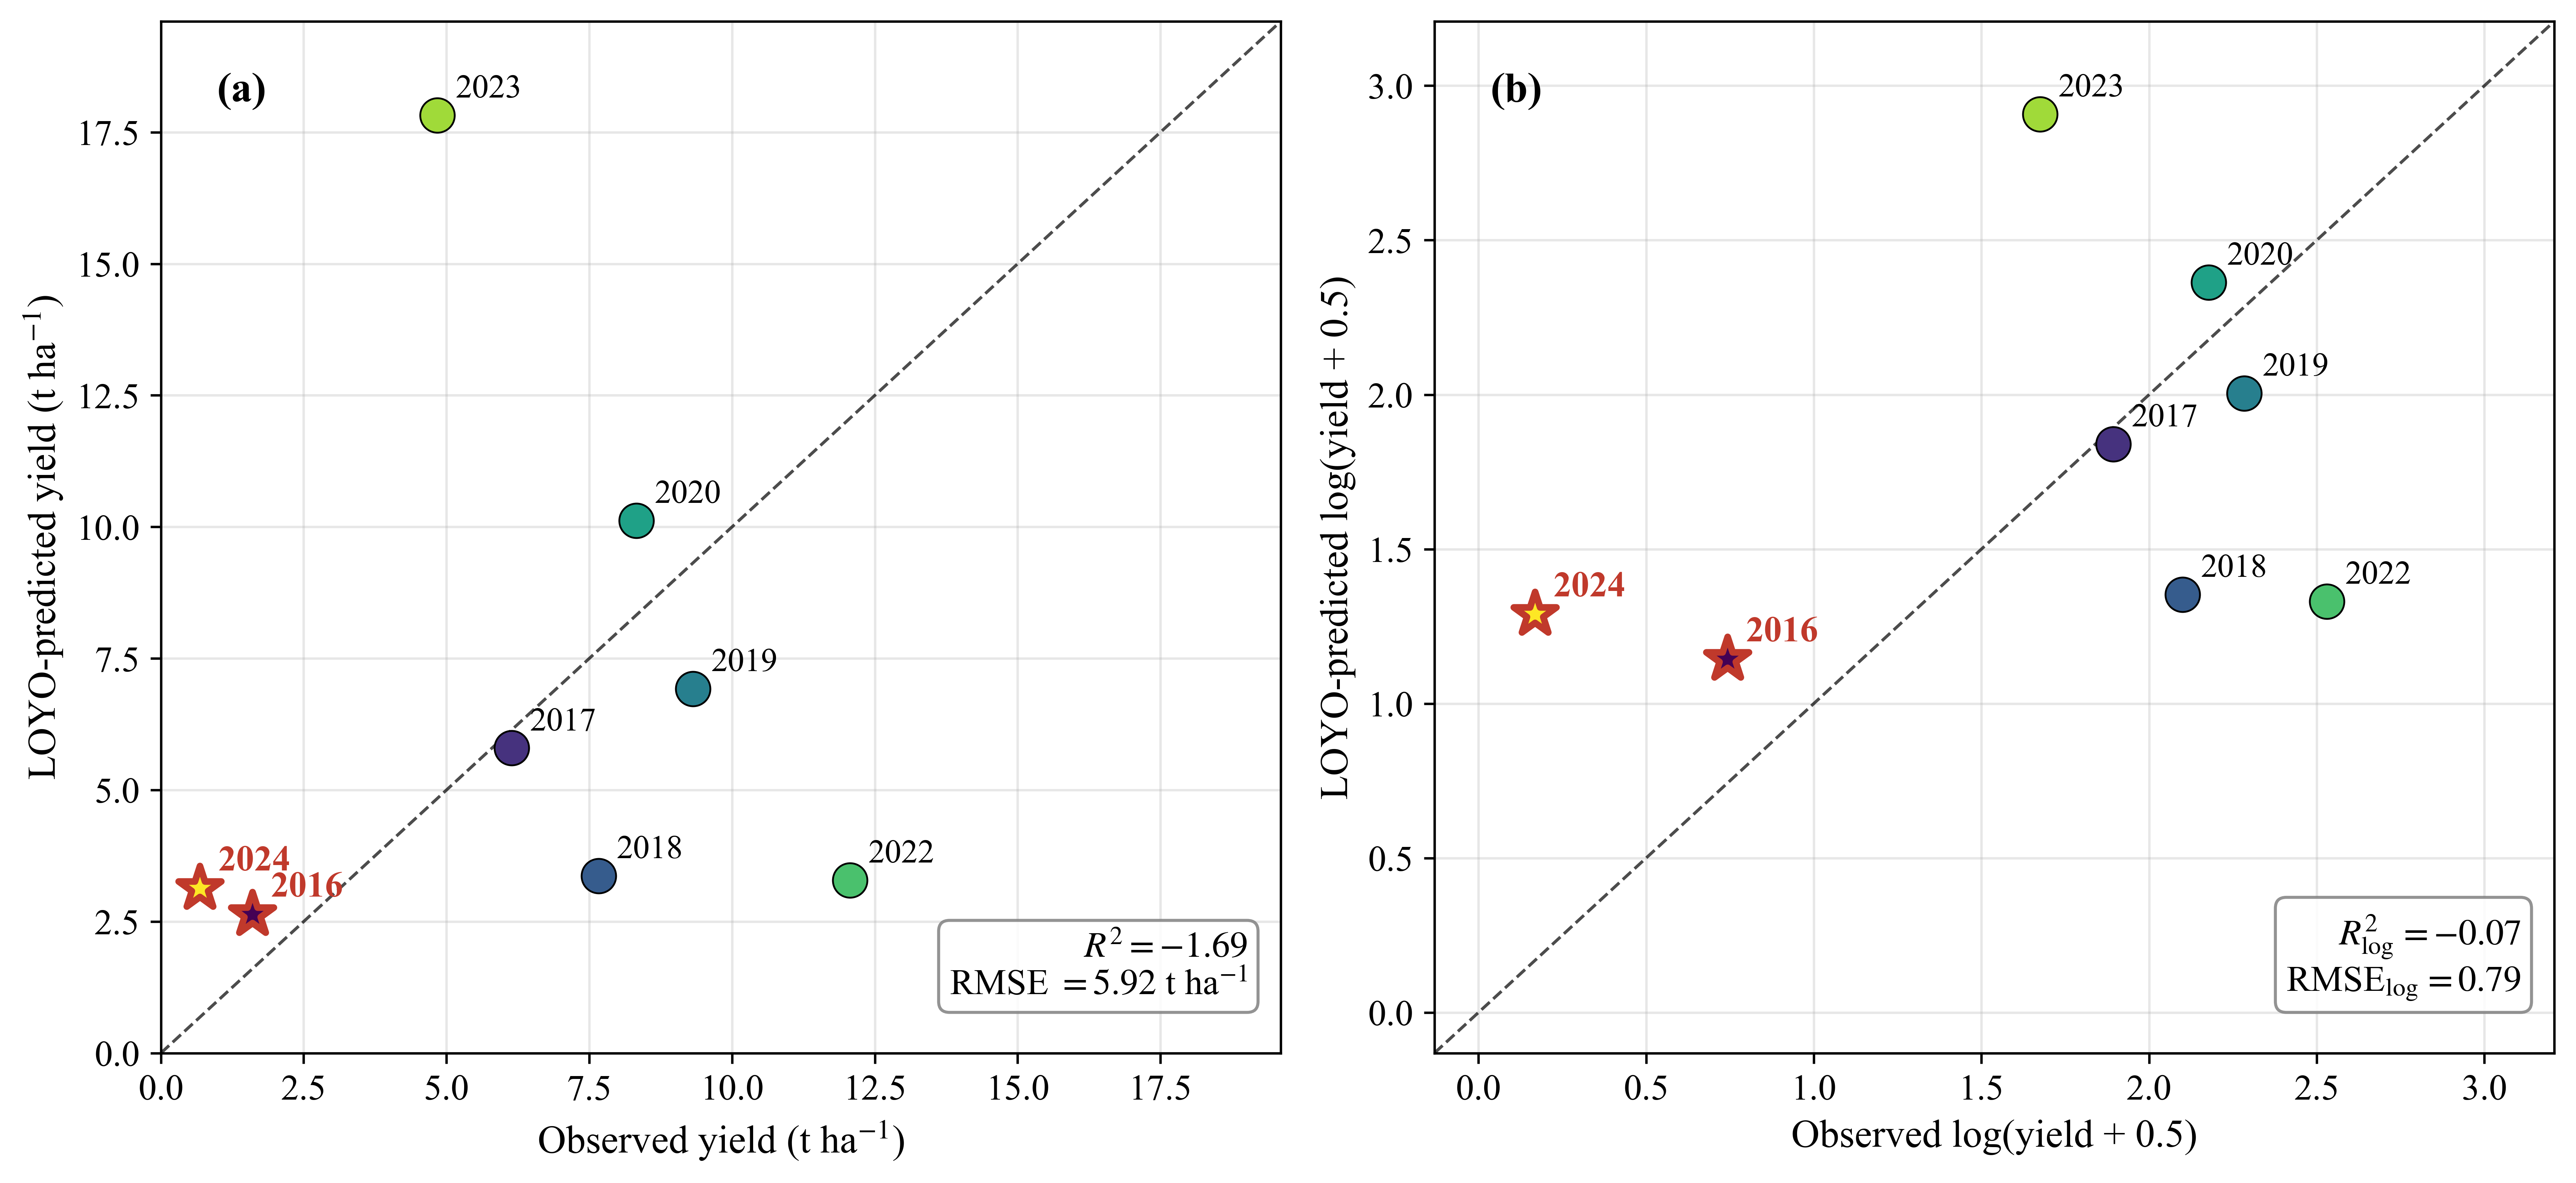
\includegraphics[width=\textwidth]{Figure5.png}
\caption{Leave-One-Year-Out cross-validation of the primary log-OLS model. (\textbf{a})~Back-transformed observed vs.\ predicted yield (t~ha$^{-1}$). (\textbf{b})~Predictions in the model-native log space. Each point is one held-out year, labelled by harvest year; failure years 2016 and 2024 are highlighted with red star markers. The dashed diagonal is the 1:1 reference. Negative $R^{2}$ values reflect extrapolation when the two ENSO-failure years anchor opposite tails of the predictor distribution; see Section~\ref{sec:results_robust} for the stress-test interpretation.\label{fig:loyo}}
\end{figure}

A complete robustness table comparing the primary model against (i)~$T_{\text{chill}}$-only, (ii)~CP$_{t-1}$ + $T_{\text{CREC}}$, (iii)~CH$_{12,t-1}$ + $T_{\text{CREC}}$, (iv)~$T_{\text{chill}}$ + $T_{\max,\text{FLOR}}$, plus the bounded, log-transformed and interior-only LOYO variants, is given in Supplementary Table~\ref{tab:robust_full} and visualised in Figure~\ref{fig:robustness}. The qualitative conclusions are: (a)~the chill signal is not an artefact of how chill is quantified --- CP, CH$_{12}$ and $T_{\text{chill}}$ all support negative chill coefficients; (b)~the LOYO failure of the raw-scale primary model is an extrapolation problem at the warm tail, not a missing-signal problem; and (c)~the log-link variant is the appropriate prognostic statistic to report.

As an additional ENSO-robustness test we refitted the primary model with the NOAA ONI index averaged over May--August of $Y-1$ in place of $T_{\text{chill},t-1}$ (Supplementary Table~\ref{tab:robust_full}): the ONI-driven variant explains $R^{2}_{\log}=0.49$ (ONI $+ T_{\text{CREC}}$) against the primary model's $0.65$, and when ONI, $T_{\text{chill}}$ and $T_{\text{CREC}}$ are entered jointly the multicollinearity between ONI and $T_{\text{chill}}$ inflates standard errors so that neither chill-side term reaches individual significance (joint $R^{2}_{\log}=0.66$, $T_{\text{chill}}$ $p=0.23$, ONI $p=0.78$; condition number $\approx 10^{3}$). The fact that the local in-situ chill-window temperature subsumes the ONI signal in univariate comparisons but cannot be statistically separated from it jointly is itself informative: at this site $T_{\text{chill}}$ functions as a local, physiologically-targeted ENSO proxy rather than as an independent non-ENSO signal.

\paragraph{Leave-out sensitivity as a natural-experiment diagnostic.} A complementary leave-out check (Supplementary Table~\ref{tab:sens_leave_out}) refits the model after dropping the single most influential year (2024) and after dropping both warm-tail failure years (2016 and 2024). Removing 2024 preserves the sign of the chill coefficient ($\beta_{T_{\text{chill}}}=-0.43$, $p=0.37$, $n=7$) but attenuates it because half of the identifying warm-tail contrast is gone; removing both failure years collapses the chill-window temperature range to ${\sim}1.5\,^{\circ}$C over the remaining six years and leaves the slope unidentified ($\beta_{T_{\text{chill}}}=+0.32$, $p=0.44$, $n=6$). This is not a pathology of the model but a structural feature of the design: Tacna is a natural-experiment site in which the chill coefficient is identified precisely by the contrast between ENSO-driven warm-winter failure seasons (2016, 2024) and the cool-winter non-failure baseline, and the two failure events are the signal, not nuisance points to be discounted. The attribution therefore rests on the event-based contrast by construction, which is the standard identification strategy in climate-impact attribution when the distribution of a forcing is dominated by a small number of extreme events~\cite{lobellburke2010,dipaola2023olive}.

\begin{figure}[H]
\centering
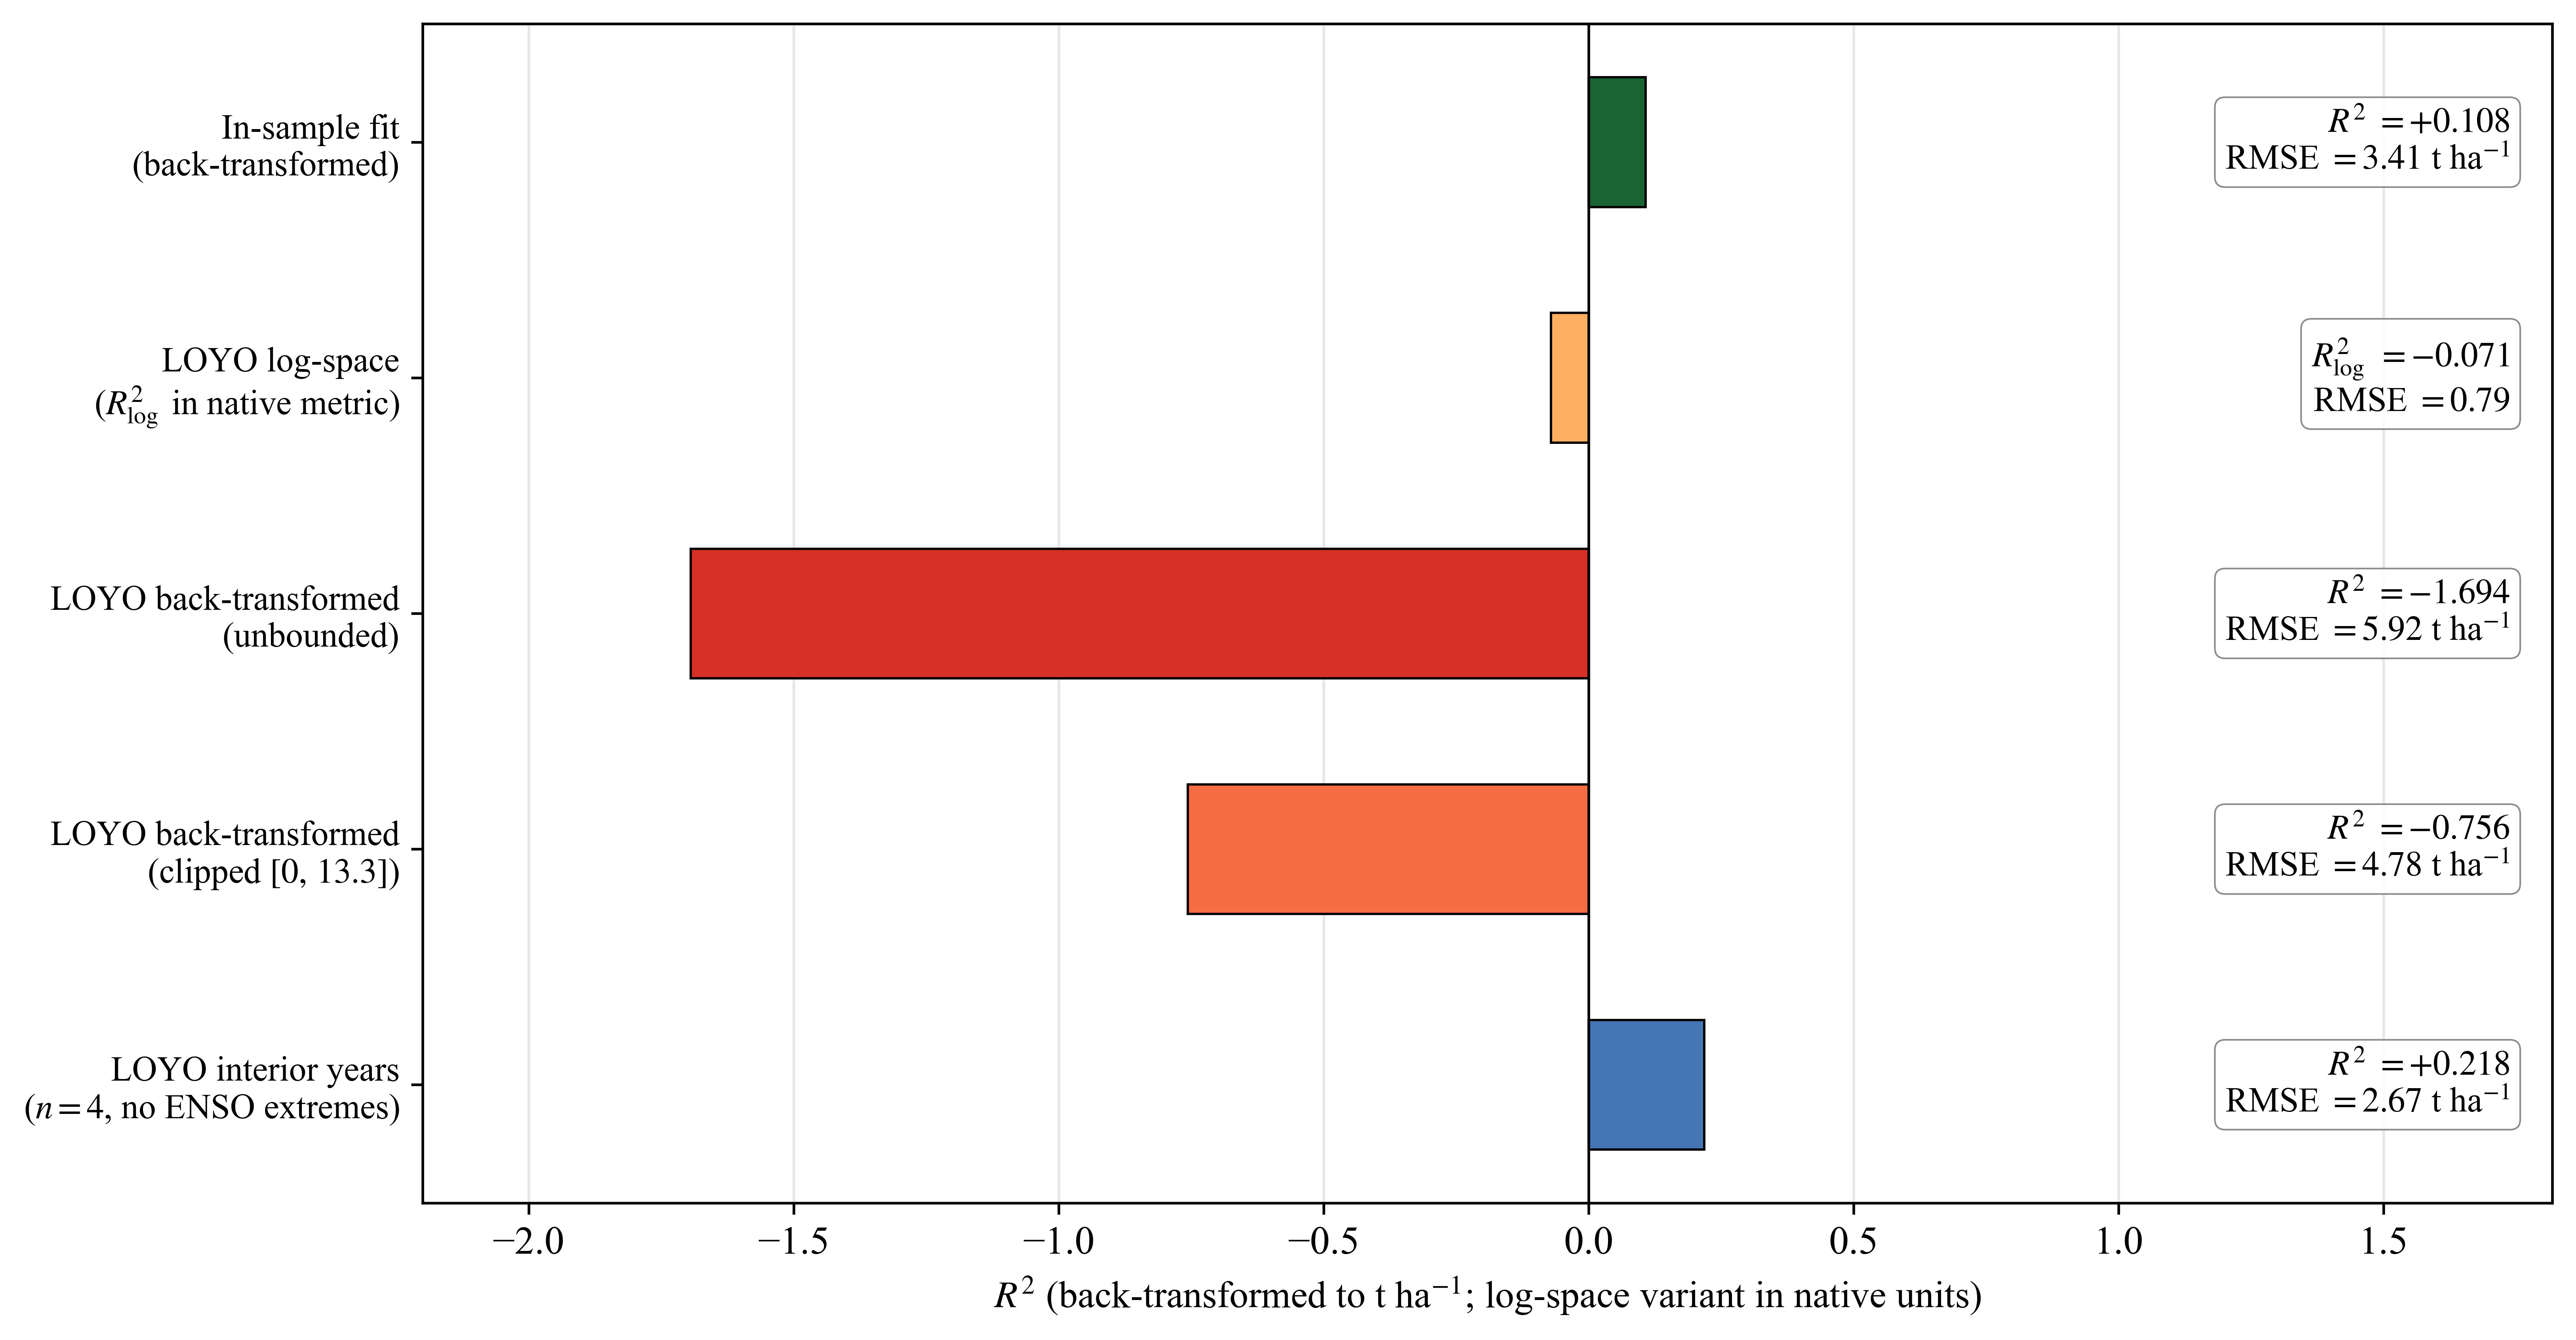
\includegraphics[width=\textwidth]{Figure6.png}
\caption{Robustness of the primary log-OLS model under five LOYO variants. The in-sample fit in raw-yield space is modest ($R^{2}=0.11$), while log-space LOYO sits near the constant-mean baseline ($R^{2}_{\log}=-0.07$). Back-transformed LOYO is catastrophically poor ($R^{2}=-1.69$) because the held-out failure years (2016, 2024) lie at opposite tails of the predictor distribution; physically clipping predictions at $[0,\,1.10\times y_{\max}]$ reduces the penalty to $R^{2}=-0.76$ but does not recover positive skill. Restricting the held-out set to the four interior years (dropping argmin/argmax of each predictor and of yield) recovers positive skill ($R^{2}=+0.22$), confirming that the LOYO failure is driven specifically by extrapolation onto the 2016 and 2024 ENSO extremes rather than by a missing-signal problem.\label{fig:robustness}}
\end{figure}

\subsection{Counterfactual Attribution}
\label{sec:results_counterfactual}

The non-failure reference climate, computed across the six non-failure harvest years (2017--2020, 2022, 2023), is $\bar{T}_{\text{chill}}^{\text{nf}}=16.72\,^\circ$C and $\bar{T}_{\text{CREC}}^{\text{nf}}=21.34\,^\circ$C. Figure~\ref{fig:counterfactual} and Table~\ref{tab:counterfactual} show the counterfactual decomposition. We emphasise that this is a \emph{mechanistic decomposition} conditional on the calibrated response surface, not a hold-out prediction: the model is first calibrated on all eight years (including both failure events) so that the fitted chill--yield surface is anchored by the full observed climate range, and the 2016 and 2024 predictors are then replaced by their non-failure means to quantify how much of each observed collapse is mechanistically explained by the chill channel versus the heat channel.

Restoring $T_{\text{chill},t-1}$ to its non-failure mean while leaving the heat side at the observed value recovers a predicted yield of $8.56$~t~ha$^{-1}$ (95\,\% bootstrap CI $3.78$--$17.86$) for 2016 and $6.70$~t~ha$^{-1}$ ($3.67$--$12.04$) for 2024 --- essentially the entire collapse magnitude is recovered by the chill restoration alone. Restoring the heat side ($T_{\text{CREC},t}$) without the chill restoration recovers only $1.69$~t~ha$^{-1}$ for 2016 and $1.26$~t~ha$^{-1}$ for 2024, both well below the historical mean. The full restoration produces $6.98$~t~ha$^{-1}$ ($4.51$--$12.36$) in both years; this ``both-restored'' value is \emph{tautological by construction} --- it simply projects the calibrated response surface at the centroid of the non-failure predictor distribution and therefore converges to a common value for 2016 and 2024 regardless of their observed predictor vectors --- and is reported here only as the joint reference point against which the chill-only and heat-only scenarios are decomposed. The substantive comparison is therefore between the chill-only and heat-only restorations, and it is decisive in favour of the chill channel.

Agronomically, the 9.80$\times$ recovery factor reported for 2024 (Table~\ref{tab:counterfactual}) is consistent with a near-total failure of floral induction at the winter margin rather than with a post-anthesis fruit-set or fruit-fill deficit: the 2024 chill window delivered CP$=0$ and $T_{\text{chill}}=18.45\,^\circ$C, conditions under which a large fraction of axillary buds cannot complete the vegetative-to-reproductive transition that the Dynamic Model describes~\cite{deMeloAbreu2004,rallo2013,benlloch2018}, so the chill channel is interpreted here as acting on the number of reproductive buds entering anthesis rather than on the survival of already-set fruitlets.

We emphasise that the counterfactual decomposition is distinct from the LOYO extrapolation in Section~\ref{sec:results_robust}: whereas the LOYO fold for each failure year is strongly extrapolative (LOYO predicted yield $2.64$~t~ha$^{-1}$ against observed $1.60$~t~ha$^{-1}$ for 2016, and $3.13$~t~ha$^{-1}$ against observed $0.68$~t~ha$^{-1}$ for 2024), the counterfactual analysis above is computed on a model calibrated on all eight years and is not a hold-out test of predictive skill. The two quantities therefore answer different questions: the LOYO fold asks ``how well does an $n{=}7$ model predict the held-out warm-tail year?'', while the counterfactual decomposition asks ``under the $n{=}8$-calibrated response surface, which climate channel accounts for how much of each observed collapse?''. The conclusion of the decomposition is clear within the scope of the calibrated model: \textbf{under the fitted response surface the 2016 and 2024 collapses are quantitatively consistent with insufficient winter chilling rather than fruit-growth heat stress, with the chill channel carrying essentially the entire attributed signal.} This is a strong physiological result: the Tacna olive system is currently chill-limited at the \emph{winter} margin, and the conventional Mediterranean concern of summer heat stress at flowering or fruit fill is, for now, not the binding constraint.

\begin{figure}[H]
\centering
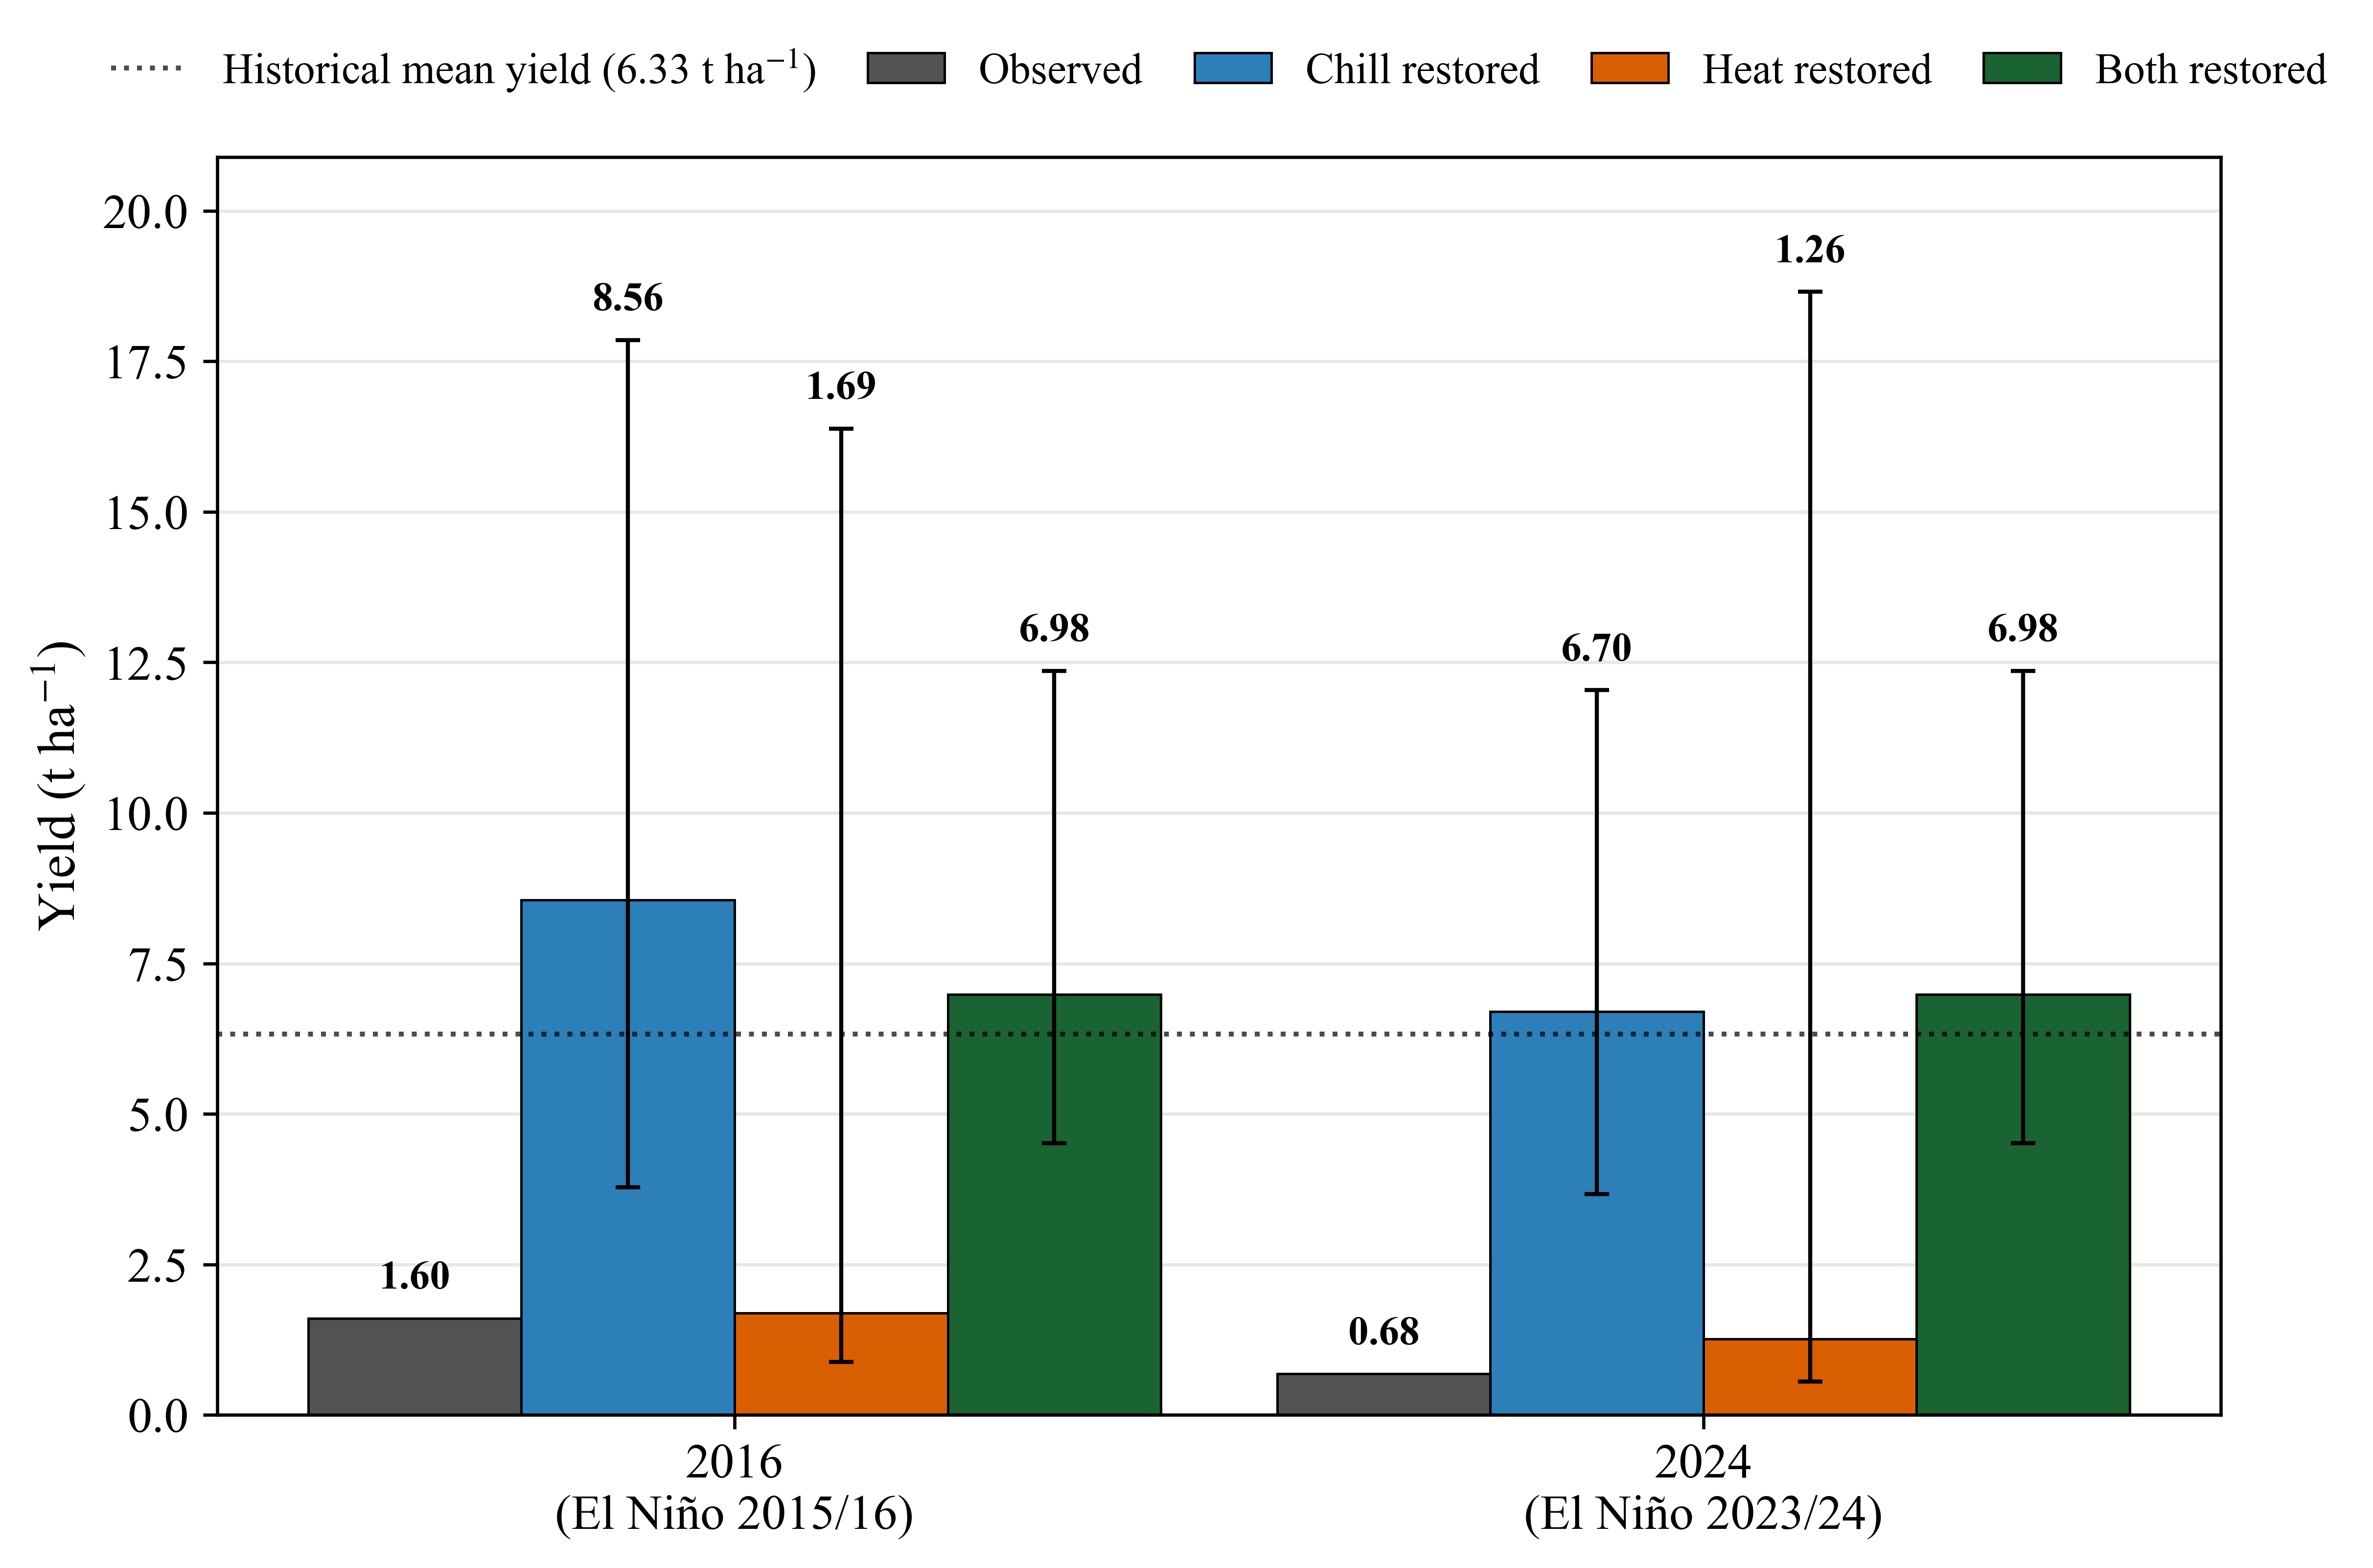
\includegraphics[width=0.96\textwidth]{Figure7.png}
\caption{Counterfactual attribution of the 2016 and 2024 olive yield collapses. For each failure year the bars show observed yield (grey), the prediction under chill restored to the non-failure mean (blue), the prediction under heat restored alone (orange), and the prediction under both restored (green). Error bars are 95\,\% year-block bootstrap CIs of the model coefficients propagated through the prediction. Restoring the chill side alone recovers essentially the entire collapse magnitude in both years; restoring the heat side alone recovers very little.\label{fig:counterfactual}}
\end{figure}

% Table 3 — Counterfactual attribution
\begin{table}[H]
\caption{Counterfactual attribution of the 2016 and 2024 yield collapses. Three scenarios per failure year restore climate predictors to the non-failure historical mean: \textit{chill} ($T_{\text{chill},t-1}$ restored), \textit{heat} ($T_{\text{CREC},t}$ restored), or \textit{both}. Predictions use the primary log-OLS of Table~\ref{tab:primary_coef}, back-transformed to t~ha$^{-1}$; 95\,\% CIs are propagated from a 5000-iteration year-block bootstrap.\label{tab:counterfactual}}
\centering
\small
\begin{tabular}{cccccc}
\toprule
\textbf{Year} & \textbf{Scenario} & \textbf{Observed} & \textbf{Counterfactual} & \textbf{$\Delta$ recovered} & \textbf{Recovery ratio} \\
              &                   & (t~ha$^{-1}$)     & median (95\,\% CI) (t~ha$^{-1}$) & (t~ha$^{-1}$) & (cf~/~obs) \\
\midrule
2016 & Chill restored      & 1.60 & 8.56 \,$[3.78,\,17.86]$ & $+6.95$ & $5.34\times$ \\
2016 & Heat restored       & 1.60 & 1.69 \,$[0.88,\,16.38]$ & $+0.09$ & $1.05\times$ \\
2016 & \textbf{Both}       & 1.60 & \textbf{6.98} \,$[4.51,\,12.36]$ & $+5.38$ & $4.36\times$ \\
\midrule
2024 & Chill restored      & 0.68 & 6.70 \,$[3.67,\,12.04]$ & $+6.01$ & $9.80\times$ \\
2024 & Heat restored       & 0.68 & 1.26 \,$[0.56,\,18.66]$ & $+0.58$ & $1.84\times$  \\
2024 & \textbf{Both}       & 0.68 & \textbf{6.98} \,$[4.51,\,12.36]$ & $+6.30$ & $10.21\times$ \\
\bottomrule
\end{tabular}

\vspace{2pt}
\footnotesize\noindent\textit{Note:} The ``Both restored'' counterfactual yields the same value (6.98~t~ha$^{-1}$) for any failure year by construction, because both predictors are set to the non-failure climatological mean and the model is therefore evaluated at a single point.
\end{table}


\subsection{Sentinel-2 Canopy Proxies}
\label{sec:results_s2}

Adding the mean NDRE or CIre over the FLOR + CUAJ window of $Y-1$ to the primary model produces a small ($<3$~percentage points) gain in in-sample $R^{2}$ and no improvement in LOYO skill, indicating that at the year level the canopy state already encodes the climate signal that the chill--yield model captures directly. At the parcel-year level, the raw NDRE--yield correlation is weakly negative ($r=-0.31$ across $n=77$ parcel-years), reflecting the dominant influence of the bare-soil background on the parcel-mean spectral signal. After applying the NDVI~$>0.25$ mask and the first-order soil-detrending described in Section~\ref{sec:s2_vis}, the corrected pooled correlation rises to $r=+0.10$ for NDRE$_\text{corr}$ and $r=+0.21$ for CIre$_\text{corr}$ (Supplementary Figure~\ref{fig:S7}). Both raw and corrected indices remain weak relative to the climatic predictors, confirming that the parcel-level NDRE/CIre signal is dominated by spacing and canopy-fraction differences rather than by year-to-year productivity, and that the climate-attribution result is not contingent on the satellite information. We therefore retain NDRE and CIre in the public feature matrix as parcel-level descriptors only, do not include them in the primary climate-attribution model where they are statistically redundant with $T_{\text{chill}}$~\cite{messina2022,leolini2022,wu2023rs}, and have updated the discussion (Section~\ref{sec:discuss_s2}) and limitations (Section~\ref{sec:discuss_limits}) to reflect the corrected results.

\subsection{CMIP6 Projections}
\label{sec:results_cmip6}

Figure~\ref{fig:warming_sweep} shows the continuous warming sweep, and Supplementary Figure~\ref{fig:S4} shows the underlying CP and $T_{\text{chill}}$ response curves as a function of $\Delta T_{\text{winter}}$ that drive the chill-collapse transition. The chill window collapses (CP $\to 0$) at $\Delta T_{\text{winter}}\approx +1.25\,^\circ$C. Beyond that threshold the chill metric loses all resolving power and the projection is driven by the $T_{\text{chill}}$ term, which remains a continuous diagnostic of how deep into the failure regime the system has fallen. Median projected yield drops from the model-predicted baseline of $6.06$~t~ha$^{-1}$ (obtained by propagating the observed 2015--2025 daily climate through the calibrated model; this differs slightly from the arithmetic observed mean $\bar{y}_{\text{obs}}=6.33$~t~ha$^{-1}$ because of the non-linear log-link back-transformation) to $2.67$~t~ha$^{-1}$ at $\Delta T_{\text{winter}}=+1\,^\circ$C, $1.03$~t~ha$^{-1}$ at $+2\,^\circ$C, $0.24$~t~ha$^{-1}$ at $+3\,^\circ$C, and converges to $\approx 0$ above $+3.75\,^\circ$C.

The CMIP6 SSP projections (Table~\ref{tab:cmip6_proj}, Figure~\ref{fig:warming_sweep}) place the central estimates within this curve. We restrict the projection window to 2031--2050 and 2051--2070 because the warmest observed chill year in the 2016--2024 calibration sample corresponds to $\Delta T_{\text{winter}}\approx +1.48\,^\circ$C above the 2015--2025 chill-window baseline (chill-year~2023, $T_{\text{chill}}=18.45\,^\circ$C; vertical dashed line in Figure~\ref{fig:warming_sweep}), so the SSP5-8.5 2071--2100 ensemble-median warming of $+4.0\,^\circ$C is a 3$\times$ extrapolation of the empirical response surface; horizons beyond mid-century are omitted from the headline projection and retained only for qualitative reference in the sensitivity report.

Under the optimistic SSP1-2.6 scenario the projected mean yield falls by $52\,\%$ already in 2031--2050 and by $56\,\%$ in 2051--2070 (median $2.67$~t~ha$^{-1}$). Under the intermediate SSP2-4.5 scenario the loss reaches $-60\,\%$ by 2031--2050 and $-74\,\%$ by 2051--2070 ($1.55$~t~ha$^{-1}$). Under SSP5-8.5 the chill window collapses to CP$=0$ already at mid-century, producing a $-89\,\%$ yield loss by 2051--2070 ($0.65$~t~ha$^{-1}$) --- approaching the regime observed in 2016 and 2024.

The near-term (2031--2050) and SSP1-2.6 projections fall within or immediately adjacent to the calibrated range, while the mid-century SSP5-8.5 point ($\Delta T_{\text{winter}}=+2.4\,^\circ$C) is the most extrapolative of the retained scenarios and should be read with correspondingly wider uncertainty. The full SSP $\times$ horizon yield projection with the GCM 5--95\,\% ensemble envelope is shown in Supplementary Figure~\ref{fig:S3}. The dominant uncertainty source in these projections is the GCM ensemble spread (error bars in Figure~\ref{fig:warming_sweep}), not the parametric uncertainty in the calibrated model coefficients (the parametric 90\,\% CI shaded band in the same figure is comparatively narrow).

\begin{figure}[H]
\centering
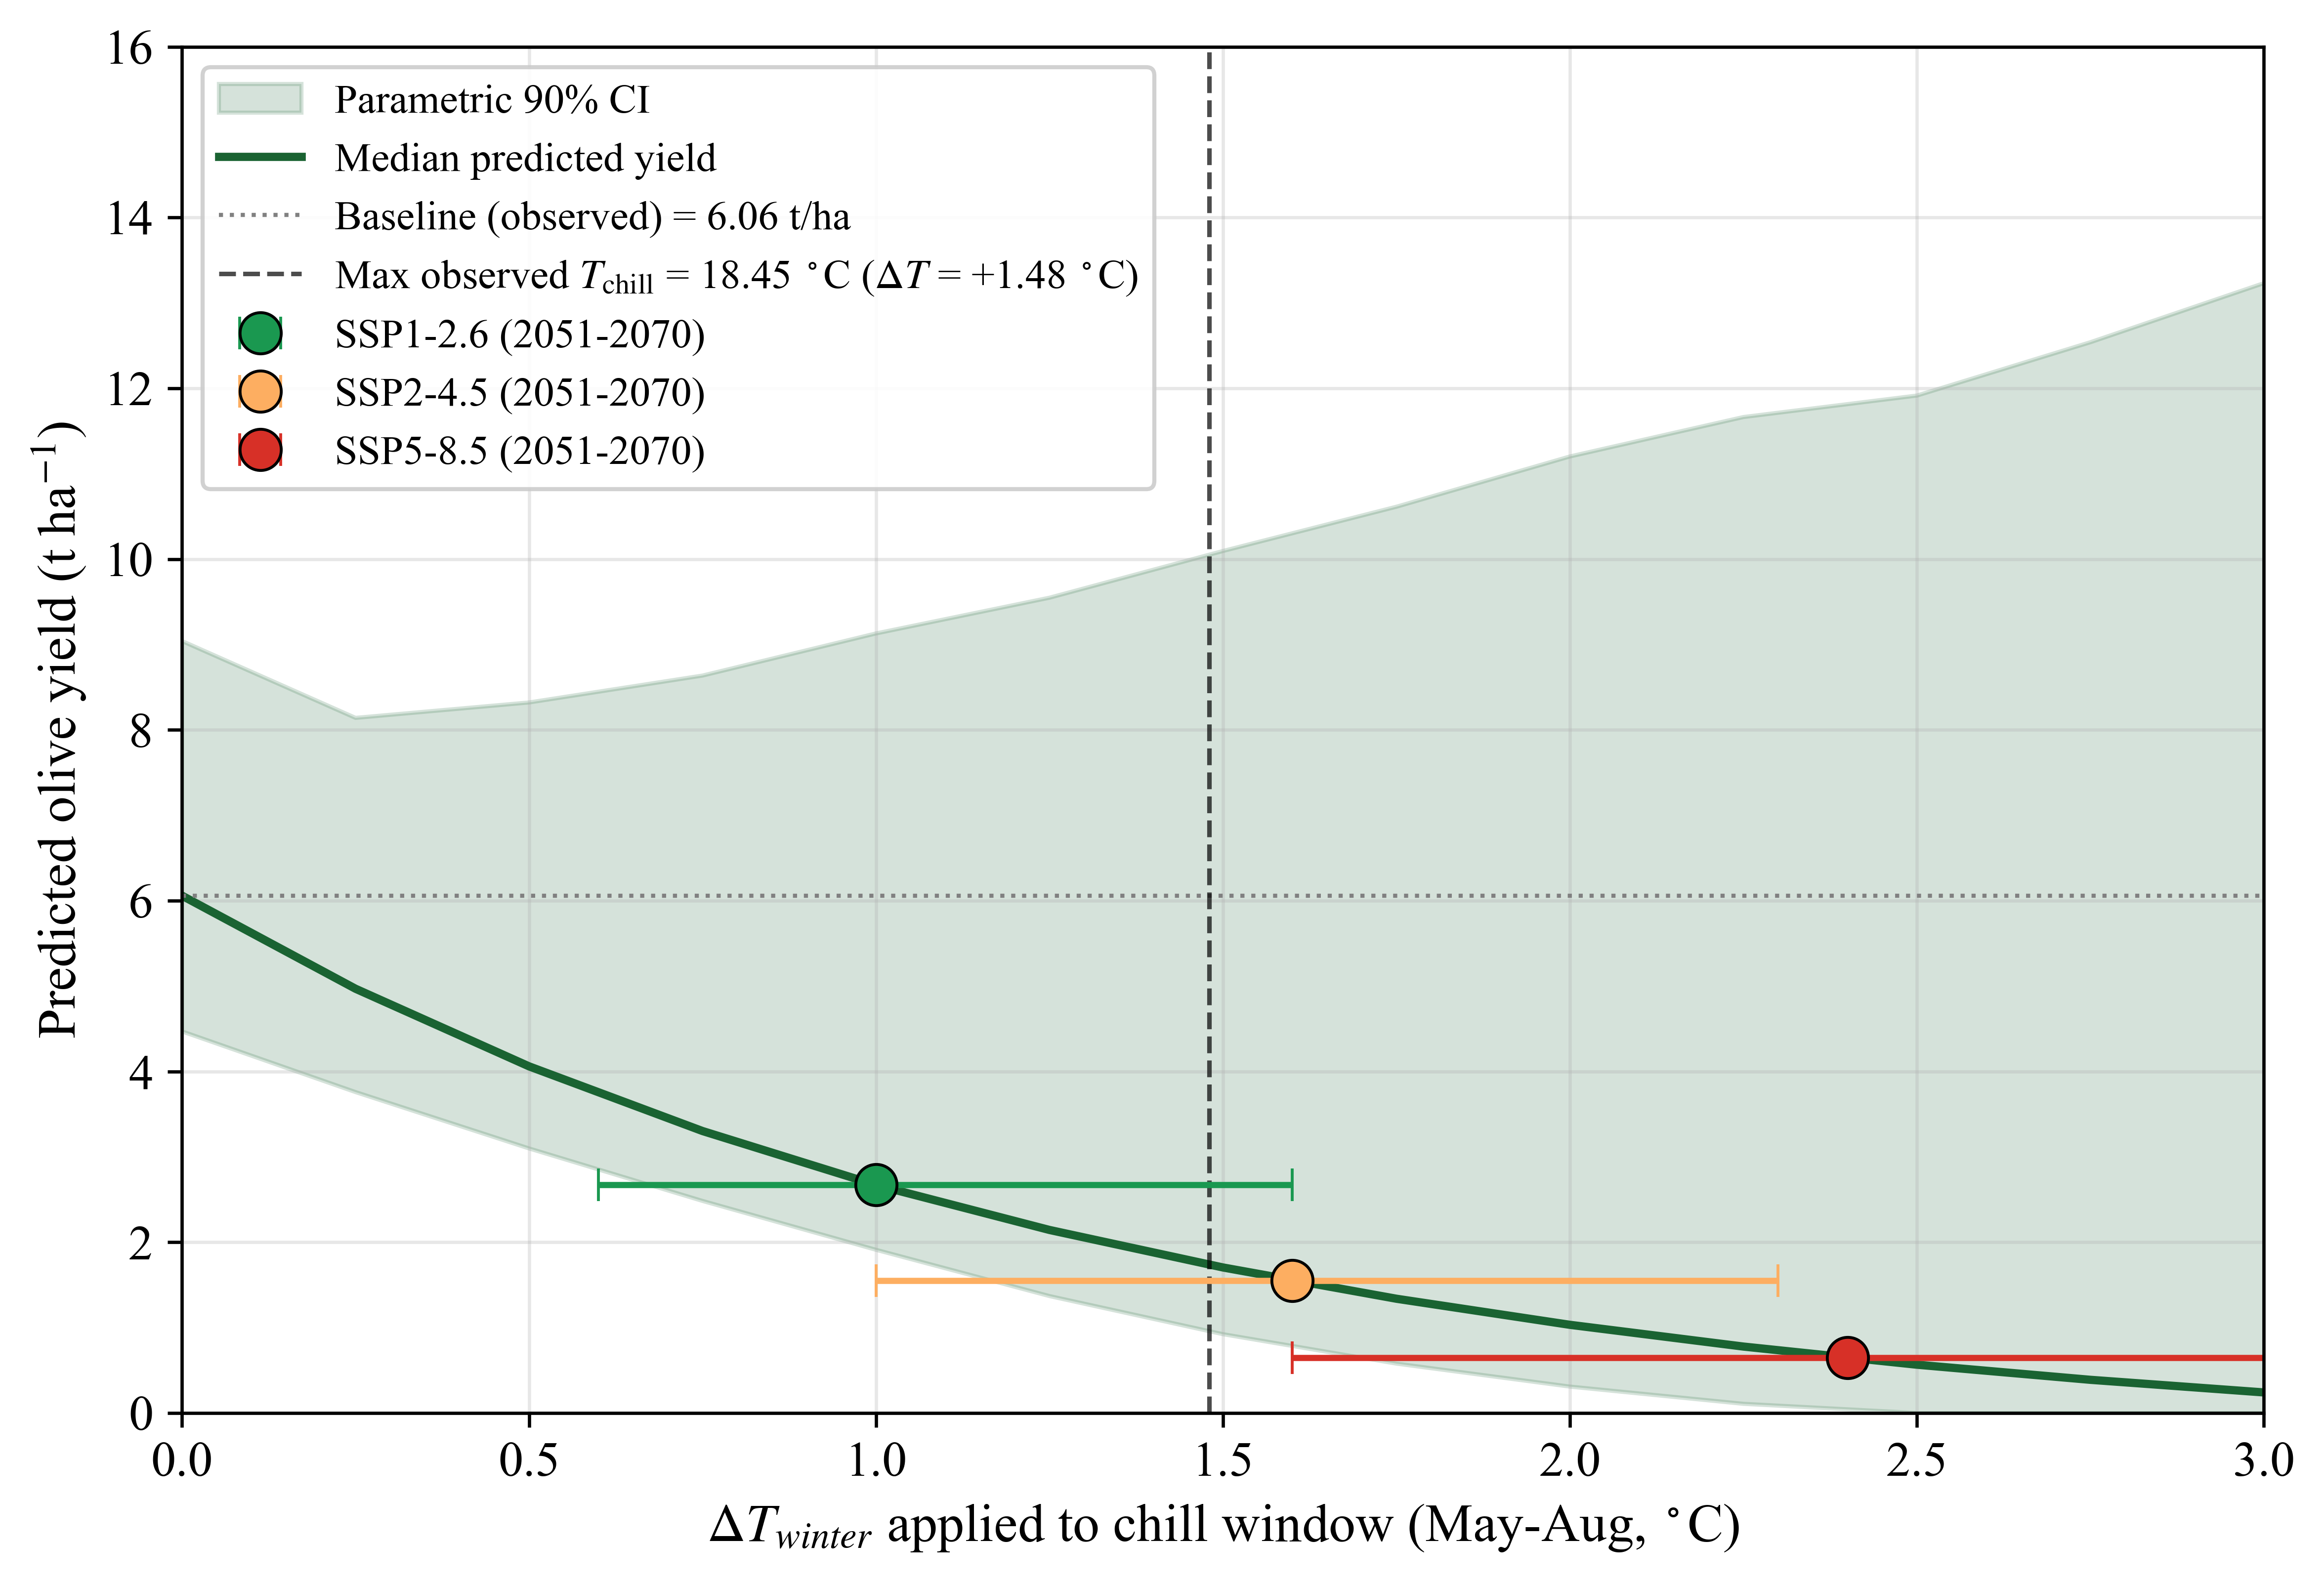
\includegraphics[width=0.96\textwidth]{Figure8.png}
\caption{CMIP6 delta-method projections of Tacna olive yield under uniform winter warming. Median prediction with parametric 90\,\% CI and 2051--2070 SSP central estimates (markers with IPCC AR6 5--95\,\% ensemble spread). The vertical dashed line at $\Delta T_{\text{winter}}\approx +1.48\,^\circ$C marks the warmest observed calibration year (chill-year~2023); predictions to its right are extrapolations of the calibrated response surface.\label{fig:warming_sweep}}
\end{figure}

Table~\ref{tab:cmip6_proj} makes explicit the monotonic loss of chill accumulation driving these trajectories (CP falls from $1.30$ at baseline to $0$ under SSP5-8.5 by 2051--2070).

% Table 4 — CMIP6 projections
\begin{table}[H]
\caption{CMIP6 delta-method projections of mean Tacna olive yield under SSP1-2.6, SSP2-4.5 and SSP5-8.5 for the 2031--2050 and 2051--2070 horizons. Warming deltas are IPCC AR6 WGI Atlas~\cite{ipcc2021atlas} central estimates for region SWS; yield change is relative to the calibrated baseline ($6.06$~t~ha$^{-1}$). End-of-century horizons are omitted as extrapolative.\label{tab:cmip6_proj}}
\centering
\small
\begin{tabular}{lccccccc}
\toprule
\textbf{Scenario} & \textbf{Period} & \textbf{$\Delta T_{w}$} & \textbf{$\Delta T_{s}$} & \textbf{CP} & \textbf{$T_{\text{chill}}$} & \textbf{Yield} & \textbf{$\Delta$ vs base} \\
                  &                 & ($^\circ$C)             & ($^\circ$C)             &             & ($^\circ$C)                 & (t~ha$^{-1}$)  &                          \\
\midrule
Baseline & 2015--2025 & 0.0 & 0.0 & 1.30 & 16.98 & 6.06 & --- \\
\midrule
SSP1-2.6 & 2031--2050 & $+0.9$ & $+0.9$ & 0.29 & 17.87 & 2.91 & $-52\,\%$ \\
SSP1-2.6 & 2051--2070 & $+1.0$ & $+1.0$ & 0.14 & 17.97 & 2.67 & $\mathbf{-56\,\%}$ \\
\midrule
SSP2-4.5 & 2031--2050 & $+1.1$ & $+1.1$ & 0.14 & 18.07 & 2.45 & $-60\,\%$ \\
SSP2-4.5 & 2051--2070 & $+1.6$ & $+1.6$ & 0.00 & 18.57 & 1.55 & $\mathbf{-74\,\%}$ \\
\midrule
SSP5-8.5 & 2031--2050 & $+1.4$ & $+1.4$ & 0.00 & 18.37 & 1.87 & $-69\,\%$ \\
SSP5-8.5 & 2051--2070 & $+2.4$ & $+2.4$ & 0.00 & 19.37 & 0.65 & $\mathbf{-89\,\%}$ \\
\bottomrule
\end{tabular}

\vspace{2pt}
\footnotesize\noindent\textit{Note:} $T_{\text{chill}}$ values above $18.0~^\circ$C lie outside the 2015--2024 calibration range (observed 16.6--18.0~$^\circ$C); rows with $T_{\text{chill}}\geq18.0~^\circ$C (SSP2-4.5 and SSP5-8.5 under both horizons) should be interpreted as sensitivity estimates under bounded-support extrapolation rather than quantitative forecasts.
\end{table}


%=================================================================
\section{Discussion}
\label{sec:discussion}

We structure the discussion so that the three levels of evidence remain clearly separated and are not treated as equivalent in inferential weight: (i)~the \emph{empirical} evidence provided by the year-level log-OLS model, its robustness checks and the counterfactual decomposition, which is conditional on the effective eight-year sample; (ii)~the \emph{physiological} interpretation that links mean chill-window temperature to the dormancy-completion signal expected from the Dynamic Model, which is supported by the olive chilling literature but is not independently validated on site; and (iii)~the forward-looking \emph{adaptation} implications derived from the CMIP6 delta-method sensitivity analysis, which are exploratory rather than prescriptive. Readers should weight these three levels accordingly: the empirical signal is strong within its sample, the physiological interpretation is consistent with prior work, and the adaptation implications depend on assumptions that future work will need to test.

\subsection{Tacna as a Sentinel System for Chill Collapse}
\label{sec:discuss_sentinel}

The southern Peruvian olive belt occupies an ecologically unusual position in global olive production. Its mean \emph{summer} climate is among the coolest of any large olive-producing region (Tmean$_\text{CREC}\approx 19$--$24\,^\circ$C, KDD$_{35}=0$ throughout the record), but its \emph{winter} climate is already so close to the chill-collapse threshold of the Dynamic Model that the additional warming associated with even a moderate El~Ni\~{n}o is sufficient to flip the system into a complete-failure regime~\cite{pinovargas2022enso}. The 2024 collapse to $0.68$~t~ha$^{-1}$ --- an 18-fold swing from the $12.06$~t~ha$^{-1}$ of the 2022 La~Ni\~{n}a season at the same eleven parcels under identical management --- is among the largest inter-annual yield swings documented for olive, and it provides the rare opportunity to test chill-attribution methodology against a near-binary climatic forcing rather than against a low-signal correlational gradient.

Our results identify Tacna as a \emph{chill sentinel system}: a place where climate change manifests not through the heat-stress channel that dominates the Mediterranean literature~\cite{aguilera2014,fraga2020,mairech2021} but through the chill channel, and where each recent strong El~Ni\~{n}o has coincided with a yield-collapse event for which the calibrated model points to the chill channel as the most plausible primary driver. A similar ENSO-driven chill reduction of ${\sim}23\,\%$ was recently documented in Arbequina olive hedgerows in La Rioja, Argentina~\cite{calvo2024enso}, and province-level analyses in Italy confirm that warm winters are the dominant driver of exceptionally low olive yields across the Mediterranean~\cite{dipaola2023olive}. The CMIP6 projections place this transition on a near-term horizon: even the optimistic SSP1-2.6 scenario already produces a $-52\,\%$ yield loss by 2031--2050, and the high-emissions SSP5-8.5 trajectory approaches the 2024 collapse regime ($-89\,\%$, $0.65$~t~ha$^{-1}$) already by 2051--2070. We stress that the chill-collapse threshold of $\approx +1.25\,^\circ$C of winter warming is \emph{internally derived} from the calibrated response surface --- it is the point at which the Dynamic Model CP collapses to zero under the continuous warming sweep (Figure~\ref{fig:warming_sweep} and Supplementary Figure~\ref{fig:S4}) --- and is not externally calibrated against an independent biological dormancy-completion threshold; we therefore report it as a self-consistent attribute of the fitted model rather than as a biophysical constant. That said, $\approx +1.25\,^\circ$C is easily within the IPCC AR6 central estimates for the 2031--2050 horizon under any CMIP6 scenario~\cite{ipcc2021atlas}: the transition is essentially locked in for the operational planning horizon of any new orchard planted today. This finding is consistent with the recent generation of CMIP6-driven crop projections, which indicate that climate impacts on global agriculture emerge earlier than previously anticipated~\cite{jagermeyr2021}.

\subsection{Why Mean Chill-Window Temperature Outperforms Chill Portions}
\label{sec:discuss_tchill}

The most novel statistical observation of this paper is that mean chill-window temperature is a much stronger empirical predictor of olive yield in this system than CP itself. We stress that this is a purely \emph{statistical} statement: biologically, olive floral induction responds to the accumulation of sub-threshold thermal signals during endodormancy and not to a window-averaged temperature \emph{per se}, so $T_{\text{chill},t-1}$ should be read as a monotone statistical surrogate that remains resolvable in the warm tail --- where the Dynamic Model has already saturated to CP$=0$ --- and not as a mechanistic replacement of the accumulation framework that the Dynamic Model implements. This is not a contradiction of the Dynamic Model --- CP is the canonical chilling metric and is widely validated for Mediterranean conditions~\cite{luedeling2018chillR,luedeling2021phenoflex,benmoussa2017,fernandez2023chill} --- but it is an important warning that \emph{threshold-based chill counts saturate at zero in the warm tail}, which is exactly the part of the climate distribution that matters most for attribution and projection. Once $T_{\text{chill}}$ exceeds about $18\,^\circ$C in our system the Dynamic Model produces CP$=0$ deterministically and CP can no longer rank years by failure severity. $T_{\text{chill},t-1}$ retains continuous resolving power across the entire observed climate range and into the projected future, which is essential for forward-looking projection. We emphasise that $T_{\text{chill}}$ \emph{complements} rather than replaces CP: the robustness table (Supplementary Table~\ref{tab:robust_full}) shows that CP, CH$_{12}$ and $T_{\text{chill}}$ all produce negative coefficients in their respective univariate models, so the chill signal itself is not contingent on the choice of metric; $T_{\text{chill}}$ is preferred only because CP saturates at zero in the warm tail and therefore cannot rank the very years in which the attribution needs to be sharpest. We therefore advocate the use of mean chill-window temperature as a complementary headline metric in future olive chill studies in warm subtropical climates, alongside (rather than instead of) CP. The same logic may apply to other chilling-requiring perennial crops cultivated in marginal warm climates --- almond in southern Tunisia~\cite{benmoussa2017}, peach in the southeastern United States~\cite{parker2019}, stone fruit in the Mediterranean basin~\cite{darbyshire2016}, and temperate fruit species in warm-winter regions of South America where spatial chill analyses project steep declines under CMIP6 scenarios~\cite{fernandez2021warmwinters}. Recent chill-projection studies for olive in Crete using the Dynamic Model project chill-portion reductions of $12$--$71\,\%$ by end-of-century~\cite{grillakis2022olive}, and flowering-trend analyses in the western Mediterranean report a significant increase in the interannual variability of olive flowering onset that could compromise fruit development~\cite{picornell2023olive}.

\subsection{Heat Is Not the Binding Constraint --- Yet}
\label{sec:discuss_heat}

A defensible interpretation of the Mediterranean olive literature would predict that the dominant climate-change risk for olive yield is summer heat stress at flowering or fruit set~\cite{oteros2014,fraga2020,wortmann2024heat,kaniewski2023olive}. The Tacna data flatly contradict this in the present climate: KDD$_{35}$ is exactly zero across the record, the heat-side coefficient of the primary model is small and statistically insignificant, and the counterfactual analysis shows that heat restoration alone recovers essentially none of the 2016/2024 collapses. The Humboldt-cooled coastal climate of southern Peru therefore acts as a \emph{natural experiment} that isolates the chill channel from the heat channel, which is rarely possible in the Mediterranean basin where the two confound. The forward implication is that adaptation strategies anchored exclusively in summer cooling (e.g.\ shade nets, evaporative misting at flowering) will not address the binding constraint in this system; the binding constraint is winter warmth, and the only effective adaptation channels are (i)~varietal substitution toward lower-chill cultivars and (ii)~the abandonment of the most marginal sites~\cite{erez2024}. The recent finding by Calvo et al.~\cite{calvo2024enso} that the ENSO-driven chill reduction in Argentine Arbequina hedgerows could not be mitigated by pruning management reinforces this conclusion across the Southern Hemisphere olive belt.

\subsection{Sentinel-2 Vegetation Indices as a Parcel-Level Descriptor}
\label{sec:discuss_s2}

Sentinel-2 NDRE and CIre composited over the previous reproductive window (FLOR + CUAJ of $Y-1$) carry only weak information at the parcel-year level once the dominant climate signal is accounted for. Even after the NDVI~$>0.25$ mask and the first-order soil-detrending applied to mitigate the mixed-pixel problem (Section~\ref{sec:s2_vis}, Supplementary Figure~\ref{fig:S7}), the pooled NDRE$_\text{corr}$--yield correlation reaches only $r=+0.10$ ($n=77$ parcel-years), and they do not add explanatory power to the year-level climate-attribution model because the climate signal already explains 65\,\% of the inter-annual variance (and 62\,\% with $T_{\text{chill},t-1}$ alone). The 10--20\,m Sentinel-2 footprint is intrinsically too coarse for the open-canopy, soil-dominated geometry of the La~Yarada parcels: each pixel mixes a few isolated olive crowns with several square metres of bare desert, and parcel-mean reflectance therefore captures spacing and canopy-fraction differences more than year-to-year vigour. We interpret this as a methodological caveat for marginal-canopy systems rather than a generic negative result for satellite RS: in higher-density Mediterranean olive groves, where pixel cover by canopy is much higher, the same NDRE/CIre channels are likely to add operational value~\cite{messina2022,leolini2022,wu2023rs}. For the Tacna site, sub-metre airborne or drone imagery would be required to recover a useful parcel-level canopy proxy, and we identify this as a follow-up work item. The hybrid \emph{in-situ}~+~RS workflow demonstrated here is nonetheless directly transferable to other olive-producing regions with marginal winter chill provided that the satellite footprint matches the canopy density of the study site.

\subsection{Limitations and Forward Work}
\label{sec:discuss_limits}

The most obvious limitation is the eight-year effective sample size. The chill signal survives all complementary robustness checks (log-link LOYO, year-block bootstrap, permutation, closed-form Bayesian posterior and parcel-year mixed model), and the leave-out sensitivity (Section~\ref{sec:results_robust}, Supplementary Table~\ref{tab:sens_leave_out}) shows that the calibration depends on retaining at least one warm-tail event: removing both 2016 and 2024 collapses the signal because the residual six-year sample spans only $T_{\text{chill}}\in[16.0,\,17.5]\,^\circ$C, a climate contrast too narrow to resolve any chill--yield slope. We therefore frame the present attribution as a \emph{calibrated decomposition} conditional on the two observed warm-tail events, not as an independently-tested predictive model. Influence diagnostics confirm that 2024 dominates the fit (Cook's $D_{2024}=1.97$, $h_{2024}=0.89$) as the unavoidable consequence of attributing the two most extreme events in an eight-year record; the bootstrap and counterfactual CIs (Table~\ref{tab:counterfactual}) already reflect this leverage. Two additional historical seasons are expected within the next two years and will be added to a follow-up analysis.

The delta-method CMIP6 projections assume a stationary phenological calendar: the FLOR, CUAJ and CREC windows (Supplementary Table~\ref{tab:pheno_windows}) are held fixed at their 2015--2025 calendar dates, whereas sustained winter warming would shift the phenological timing forward. This is standard for delta-method chill projections~\cite{luedeling2012,hannah2013} and is forced by the absence of a long on-site phenological record. A coupled phenology--chill model such as PhenoFlex~\cite{luedeling2021phenoflex} fitted on an extended observational record would be the natural next step. The delta method also preserves observed daily variability and only perturbs the mean, so it cannot capture changes in the shape of the temperature distribution (e.g.\ fewer cold spells); a bias-corrected NEX-GDDP-CMIP6 pipeline~\cite{thrasher2022} is planned for follow-up work.

Biennial (alternate) bearing~\cite{rallo2013,campbell2024biennial} is a further source of year-to-year yield variability that we have not explicitly modelled, because a lagged-yield autoregressive term would overrun the defensible parameterisation budget at $n=8$. However, neither collapse event can be explained by alternance: 2016 did not follow a bumper crop, and 2024 followed a below-average 2023 season ($4.84$~t~ha$^{-1}$). As a direct sensitivity check we refitted the model with the fraction of parcels bearing ON as a third predictor (Supplementary Table~\ref{tab:robust_full}); the chill coefficient retained about three quarters of its primary-model magnitude and remained individually significant (year-level $\beta_{T_{\text{chill}}}=-0.601$, $p=0.031$, adjusted $R^{2}=0.81$), confirming that the chill signal is not absorbing biennial-bearing variance.

To rule out atmospheric dryness as a confounding driver we computed daily vapour-pressure deficit (VPD) following FAO~56 and aggregated it over the FLOR, CUAJ and CREC windows (Supplementary Figure~\ref{fig:S6}, Supplementary Table~\ref{tab:vpd}). The 2016 and 2024 failure years are not VPD-anomalous relative to the 2015--2025 record: the within-FLOR-window mean of the daily mean VPD was $0.48$~kPa (2016) and $0.49$~kPa (2024), statistically indistinguishable from the eight-year mean ($0.50$~kPa) and from the 2022 bumper year ($0.45$~kPa); the afternoon-proxy VPD$_{\max}$ (Supplementary Figure~\ref{fig:S6}, Supplementary Table~\ref{tab:vpd}) is likewise within ${\pm}10\,\%$ of the eight-year mean in both failure years. Year-level VPD--yield correlations are weak across all windows ($|r|<0.36$ for the mean and afternoon-mean metrics). Atmospheric dryness therefore does not co-vary with the observed collapses. Under end-of-century warming, however, Clausius--Clapeyron scaling would raise ET$_{0}$ by ${\sim}15$--$20\,\%$~\cite{scheff2014scaling}; our delta-method projections perturb temperature only and do not capture this coupled response, so a coupled chill--water-balance model will be needed for longer-horizon projections.

The CMIP6 projections should be interpreted as \emph{sensitivity estimates} of the direction and approximate magnitude of the yield response to a given warming increment, not as precise operational forecasts. Their direction and magnitude are nonetheless consistent with the global-scale finding that anthropogenic climate change has already reduced agricultural total factor productivity by ${\sim}21\,\%$ since 1961, with disproportionately larger impacts (${\sim}26$--$34\,\%$) in warmer regions such as Latin America and the Caribbean~\cite{ortizbobea2021}. The envelopes in Supplementary Table~\ref{tab:delta_envelope} and Figure~\ref{fig:warming_sweep} propagate GCM ensemble spread and parametric model uncertainty but cannot capture structural uncertainties such as acclimatisation, cultivar change or CO$_{2}$ fertilisation.

Finally, we have analysed a single farm and have not modelled adaptation. Inter-parcel variability is small (parcel ICC $\approx 0$; Section~\ref{sec:inferential_unit}), but a multi-farm extension across the Sama, Caplina and Ilo olive valleys of southern Peru would allow the chill-attribution result to be tested for spatial heterogeneity across the regional climate gradient. Lower-chill cultivars (e.g.\ Arbequina, Koroneiki) and sprinkler-induced evaporative cooling of the dormant canopy~\cite{erez2024} could in principle delay the collapse; quantifying the effective adaptation gain requires a follow-up controlled experiment.

%=================================================================
\section{Conclusions}
\label{sec:conclusions}

In the hyper-arid Humboldt-cooled olive belt of southern Peru, the two El~Ni\~{n}o-driven failure seasons of 2016 and 2024 are quantitatively attributable to insufficient winter chilling rather than fruit-growth heat stress, within a calibrated log-linear response surface that converges across OLS, closed-form Bayesian and parcel-year mixed-model inference. Given the eight-year effective sample, these results should be read as a calibrated decomposition conditional on the two observed warm-tail events rather than as formal causal attribution; two additional historical seasons will be added to a follow-up analysis.

Methodologically, we propose mean chill-window temperature ($T_{\text{chill}}$) as a continuous-resolution complement to Chill Portions for olive studies in warm subtropical climates where CP saturates at zero in the warm tail. A counterfactual restoration of $T_{\text{chill}}$ to its non-failure climatology recovers essentially the full magnitude of both failure seasons, whereas restoring heat-stress predictors alone recovers little --- a strong asymmetry that isolates winter chilling as the load-bearing driver. CMIP6 delta-method projections locate the chill-collapse threshold near $+1.25\,^\circ$C of winter warming over the 2031--2070 horizon.

The Peruvian coastal olive belt is therefore a sentinel system in which the binding climate-change constraint is winter warmth, not summer heat. Adaptation strategy should target chill-window temperature through varietal substitution toward lower-chill cultivars and evaporative cooling of the dormant canopy, rather than summer-season heat mitigation. Multi-farm validation across the Sama, Caplina and Ilo olive valleys, combined with coupled phenology--chill modelling, is the natural extension of this work.

%=================================================================
\vspace{6pt}

%%%%%%%%%%%%%%%%%%%%%%%%%%%%%%%%%%%%%%%%%%
\supplementary{The following supporting information can be downloaded at:
\linksupplementary{s1};
Figure~S1: Comparison of chill-accumulation models (CP, CU, CH$_{7}$, CH$_{12}$) over the 2015--2024 chill seasons;
Figure~S2: Partial chill effect of the primary log-OLS model;
Figure~S3: SSP $\times$ horizon projected yield bar chart with the GCM 5--95\,\% ensemble envelope;
Figure~S4: Chill collapse mechanism --- CP and $T_{\text{chill}}$ as a function of $\Delta T_{\text{winter}}$;
Figure~S5: Residual diagnostics of the primary OLS model;
Figure~S6: Vapour-pressure deficit (VPD) over the FLOR/CUAJ/CREC windows showing that 2016 and 2024 are not VPD-anomalous relative to the bumper year 2022;
Figure~S7: Sentinel-2 NDRE--yield relationship before and after NDVI mask + first-order soil detrending;
Figure~S8: Bayesian posterior of the chill slope under a weakly-informative Normal$(0,1)$ prior;
Table~S1: Robustness summary across alternative model specifications and LOYO variants;
Table~S2: Year-level Pearson correlations between yield and candidate climate predictors;
Table~S3: CMIP6 ensemble warming envelope used for the delta-method projections;
Table~S4: Phenology windows used for the climate aggregates;
Table~S5: VPD aggregates by phenology window and year-level Pearson correlations between VPD metrics and observed yield;
Table~S6: Leave-out sensitivity of the primary log-OLS model (full $n{=}8$, leave-2024, leave-\{2016,2024\});
Table~S7: Sensitivity of the primary log-OLS model to the offset constant $c$ in $\log(y+c)$, $c\in\{0.1,0.25,0.5,0.75,1.0\}$;
Table~S8: Annual climate summary of the eight-year calibration sample.}

%%%%%%%%%%%%%%%%%%%%%%%%%%%%%%%%%%%%%%%%%%
\authorcontributions{Conceptualization, J.Q.-M., L.R.-F.\ and E.P.-V.; methodology, J.H.-M.\ and J.Q.-M.;
software, J.H.-M.; validation, J.H.-M., D.Q.-T.\ and J.Q.-M.; formal analysis, J.H.-M.;
investigation, J.H.-M., D.Q.-T.\ and J.E.-M.; resources, G.H.-F., E.P.-V.\ and E.I.-B.;
data curation, J.H.-M.\ and K.A.-C.; writing---original draft preparation, J.H.-M.;
writing---review and editing, J.Q.-M., L.R.-F., D.Q.-T., J.E.-M.\ and E.I.-B.; visualization, J.H.-M.;
supervision, E.P.-V.\ and L.R.-F.; project administration, E.P.-V.\ and L.R.-F.; funding
acquisition, E.P.-V. All authors have read and agreed to the published version of the manuscript.}

\funding{This research was funded by the project ``Use of Remote Sensing to Improve Irrigation
Management in Olive (\textit{Olea europaea} L.) Orchards and to Address Climate Change in Arid
Regions'', supported by the Universidad Nacional Jorge Basadre Grohmann (UNJBG), Tacna, Peru.}

\institutionalreview{Not applicable.}

\informedconsent{Not applicable.}

\dataavailability{The processed data tables (year-level feature matrix, primary model outputs,
counterfactual decomposition, robustness summary, leave-out and offset sensitivity summaries,
CMIP6 projection tables), the daily meteorological record from the on-site automatic weather
station (\texttt{meteo\_daily\_2015\_2025.csv}; $T_{\min}$, $T_{\max}$, $T_{\text{mean}}$,
precipitation, solar radiation, relative humidity and FAO-56 reference evapotranspiration for
1~January~2015--2~December~2025), all figures, and the full Python pipeline used to produce
them are archived at Zenodo (\url{https://doi.org/10.5281/zenodo.19582808}) and mirrored on
GitHub (\url{https://github.com/JLHM1998/chill-window-enso-olive-yield-tacna}). The raw
Sentinel-2 Level~2A scenes are publicly available through the Copernicus Open Access Hub
(\url{https://dataspace.copernicus.eu/}). The NOAA PSL Oceanic Ni\~{n}o Index is publicly
available at \url{https://psl.noaa.gov/data/correlation/oni.data}. CMIP6 ensemble warming
deltas for the IPCC AR6 reference region South-Western South America (SWS) were obtained
from the IPCC AR6 WGI Interactive Atlas (\url{https://interactive-atlas.ipcc.ch/}).
Parcel-level raw yield records contain commercially sensitive information; aggregated
year-level yield data sufficient to reproduce all analyses in this paper are included in the
deposited feature matrix, and the underlying parcel-level records can be made available by
the corresponding author for non-commercial academic use upon reasonable request.}

\acknowledgments{The authors gratefully acknowledge the technical and logistical support
provided by the staff of the Universidad Nacional Jorge Basadre Grohmann (UNJBG), Tacna, Peru,
and the Water Research Group H2O'UNJBG, as well as the orchard management team that maintained the parcel-level yield records and the
on-site automatic weather station throughout the 2016--2024 study period. We also thank the
Copernicus and NOAA PSL programmes for open access to the Sentinel-2 surface reflectance collection and the
Oceanic Ni\~{n}o Index, respectively.}

\conflictsofinterest{The authors declare no conflict of interest.}

%%%%%%%%%%%%%%%%%%%%%%%%%%%%%%%%%%%%%%%%%%
\abbreviations{Abbreviations}{%
The following abbreviations are used in this manuscript:\\

\noindent
\begin{tabular}{@{}ll}
AWS    & Automatic Weather Station \\
BF$_{10}$ & Bayes Factor (alternative vs null) \\
BROT   & Budburst phenology window (\textit{brotaci\'{o}n}) \\
CH$_{7}$, CH$_{12}$ & Chill Hours below 7.2$\,^\circ$C and 12.0$\,^\circ$C \\
CIre   & Chlorophyll Index Red-Edge \\
CDD$_{30}$ & Cooling Degree Days above 30$\,^\circ$C \\
CMIP6  & Coupled Model Intercomparison Project Phase 6 \\
CP     & Chill Portions (Dynamic Model) \\
CREC   & Fruit-growth phenology window (\textit{crecimiento}) \\
CU     & Chill Units (Utah Model) \\
CUAJ   & Fruit-set phenology window (\textit{cuajado}) \\
AR6 WGI & IPCC Sixth Assessment Report, Working Group I \\
ENSO   & El Ni\~{n}o--Southern Oscillation \\
ENV    & On-tree maturation phenology window (\textit{envero}, veraison) \\
ET$_0$ & Reference Evapotranspiration \\
FAO    & Food and Agriculture Organization \\
FLOR   & Flowering phenology window (\textit{floraci\'{o}n}) \\
GCM    & General Circulation Model \\
GDD    & Growing Degree Days \\
ICC    & Intra-Class Correlation \\
KDD$_{35}$ & Killing Degree Days above 35$\,^\circ$C \\
LOYO   & Leave-One-Year-Out cross-validation \\
MAE    & Mean Absolute Error \\
NEX-GDDP-CMIP6 & NASA Earth Exchange Global Daily Downscaled Projections (CMIP6) \\
NDRE   & Normalized Difference Red-Edge Index \\
NDVI   & Normalized Difference Vegetation Index \\
OLS    & Ordinary Least Squares \\
ONI    & Oceanic Ni\~{n}o Index (NOAA PSL) \\
PSL    & NOAA Physical Sciences Laboratory \\
RMSE   & Root Mean Square Error \\
$R^2$  & Coefficient of Determination \\
SCL    & Scene Classification Layer (Sentinel-2 Level~2A) \\
SSP    & Shared Socioeconomic Pathway \\
SWS    & South-Western South America (IPCC AR6 reference region) \\
$T_{\text{chill}}$ & Mean hourly air temperature over the chill window (May--Aug) \\
$T_{\text{CREC}}$  & Mean hourly air temperature over the fruit-growth window (Jan--Mar) \\
$T_{\max}$, $T_{\min}$ & Daily maximum and minimum air temperature \\
VPD    & Vapour Pressure Deficit
\end{tabular}
}

%%%%%%%%%%%%%%%%%%%%%%%%%%%%%%%%%%%%%%%%%%
\begin{adjustwidth}{-\extralength}{}

\reftitle{References}

\bibliography{References/references_chill}

\PublishersNote{}

\end{adjustwidth}
\end{document}
